%%%%%%%%%%%%%%%%%%%%%%%%%%%%%%%%%%%%%%%%%%%%%%%%%
% Main Document Spring 2008 Report
%%%%%%%%%%%%%%%%%%%%%%%%%%%%%%%%%%%%%%%%%%%%%%%%%
% Need ruproposal.cls which formats to Rutgers Style Guide
%\documentclass[pdflatex,12pt, oneside]{ruproposal}
%\draft
\documentclass[11pt, oneside, pdftex]{ruformat}
\renewcommand{\thefootnote}{\roman{footnote}}
\usepackage{amsmath, amstext, amsfonts, amssymb}
\usepackage[pdftex]{graphicx}
\usepackage{subfigure, longtable}
\usepackage{float}
\restylefloat{figure}
\usepackage{setspace}
\usepackage{hyperref}
\usepackage{pdflscape}
\singlespacing
\usepackage[left=2.54cm,bottom=2.00cm,top=2.00cm,right=2.54cm]{geometry}
\usepackage{chapterbib}
\usepackage{makeidx}
\makeindex
%\includeonly{titles,clustering,gaunetmod,graphrna}
\includeonly{titles,Chapter1/clustering,Chapter2/sequence,Chapter3/methodspaper,appendix_a}
%\usepackage{pdflscape}
%% For getting bibliography for each chapter!!
%% Use call in each chapter as \bibliography{biblio}
%%\usepackage[english]{babel}
%%\usepackage[latin1]{inputenc}

%%%%%%%%%%%%%%%%%%%%%%%%%%%%%%%%%%%%%
%% For Fonts in Document
%%%%%%%%%%%%%%%%%%%%%%%%%%%%%%%%%%%%%
%\usepackage{times}
%\usepackage{pslatex}
%\usepackage{newcent}
%\usepackage{palatcm}
%\usepackage{palatino}
\usepackage[T1]{fontenc}
\usepackage[scaled]{helvet}
\renewcommand*\familydefault{\sfdefault} 
% For more options go to: http://www.tug.dk/FontCatalogue/

%%%%%%%%%%%%%%%%%%%%%%%%%%%%%%%%%%%%%%%%%%%%%%%%%
% Theses
%%%%%%%%%%%%%%%%%%%%%%%%%%%%%%%%%%%%%%%%%%%%%%%%%
\begin{document}
    % Title and other sections that come before the body  of the document
    % theses-title has specific commands from ruthesis
    %  Title and other sections that come before the body  of the document
\phd
%\jointumdnj
\title{\textbf{RNA Structure Analysis via the Rigid Block Model}}
\author{Mauricio Esguerra Neira}
\campus{New Brunswick}
\program{Chemistry and Chemical Biology}
\director{Wilma K. Olson}

%% Gives the number of lines for comittee signatures.
\approvals{4}


% \copyrightpage % Do you want copyright protection?
\submissionmonth{October}   % only May, October or January
\submissionyear{2010}
%\today
%\figurespage
%\draft
%%% Abstract
\abstract{RNA structure  is at the  forefront of our  understanding of
the  origin  of  life,  and  the mechanisms  of  life  regulation  and
control. RNA plays  a primordial role in some  viruses.  Our knowledge
of the importance of RNA in cellular regulation is relatively new, and
this knowledge, along with the  detailed structural elucidation of the
translational  machine,  the  ribosome,   has  propelled  interest  in
understanding RNA  to a  level which starts  to closely  resemble that
given to proteins and DNA.

In  the  process  of  progressively  understanding  the  landscape  of
functionality of  such a  complex polymer as  RNA, one  practical task
left to  the structural  chemist is to  understand the details  of how
structure relates to large-scale  polymer processes. With this in mind
the fundamental problems which fuel  the work described in this thesis
are those of  the conformations which RNA's assume  in nature, and the
aim to understand how RNA folds.

The   RNA  folding  problem   can  be   understood  as   a  mechanical
problem. Therefore  efforts to determine its solution  are not foreign
to the  use of statistical  mechanical methods combined  with detailed
knowledge of  atomic level structure. Such methodology  is mainly used
in  this  work in  a  long-term  effort  to understand  the  intrinsic
structural features of RNA, and how they might relate to its folding.}


%%% Acknowledgments
\acknowledgements{I would first like to give a special thanks to
Yurong  Xin, whose patience,  help, and  collaboration since  the very
beginning of my joining of the Olson lab have been fundamental for the
development of this work. Also I would like to thank comments and help
with the persistence length code  to Luke Czapla, and Guohui Zheng who
were  very kind  and  prompt  in answering  in  full detail  technical
questions  concerning  their code.  Constant  help  on answering  3DNA
related  questions  were  always   kindly  and  promptly  answered  by
Xiang-Jun Lu.

I  thank Dr. Olson's extreme patience and room for freedom on carrying
out this research. Finally I thank all colleagues at the Olson lab.\\

I would like to dedicate this thesis to David and Stella Case, without
them, these words would not be.}

\quotes{
\textit{As a thing among things, each thing is equally insignificant; as
a world each one equally significant.} 

\textit{If I have been contemplating the stove, and then am told; but now all
you know is  the stove, my result does indeed  sound trivial. For this
represents the matter  as if I had studied the stove  as one among the
many, many things in the world.  But if I was contemplating the stove,
it was  my world,  and everything else  colorless by contrast  with it
...}

\textit{For it is equally possible to take the bare present image as the
worthless momentary  picture in the  whole temporal world, and  as the
true world among shadows.}

\begin{flushright}
\textbf{Ludwig Wittgenstein}
\end{flushright}

\vspace{2 cm}

\textit{As a molecule among molecules, each molecule is equally
insignificant; as a world each one equally significant.} 

\textit{If I have been contemplating RNA, and then am told; but now all
you  know  is RNA,  my  result does  indeed  sound  trivial. For  this
represents the matter  as if I had studied RNA as  one among the many,
many molecules in the world. But if I was contemplating RNA, it was my
world, and everything else colorless by contrast with it ...}

\textit{For it is equally possible to take the bare present image as the
worthless momentary picture in the whole temporal world, and as the
true world among shadows.}

\begin{flushright}
\textbf{Anonymous Chemist}
\end{flushright}

}

%\end{singlespace}

\figurespage
\tablespage

    \beforepreface % causes insertion of title, abstract, copyright
    \afterpreface
    % Now lets include the body of the document ...
    % Each file corresponds to a separate chapter.
%    %2345678901234567890123456789012345678901234567890123456789012345678901234567890
%%%%%%%%%%%%%%%%%%%%%%%%%%%%%%%%%%%%%%%%%%%%%%%%%%%%%%%%%%%%%%%%%%%%%%%%%%%%%%%%
% MAURICIO ESGUERRA NEIRA
% Ph. D. Thesis
%%%%%%%%%%%%%%%%%%%%%%%%%%%%%%%%%%%%%%%%%%%%%%%%%%%%%%%%%%%%%%%%%%%%%%%%%%%%%%%%
\chapter{Introduction}
\label{introduction} 
\bibliographystyle{nar}
%\section{RNA}
RNA plays  a primordial role  in life, and  perhaps also in  the early
history   of  its   origins  \cite{woese1967,   crick1968,  orgel1968,
  orgel2004}. In Biology RNA is  a central player in the transcription
and translation steps of what is known as its central dogma, i.e., DNA
makes  RNA   (via  transcription)   and  RNA  makes   protein  (during
translation).
%A  first RNA  step  transcribes  the genetic  message
%written in the DNA alphabet, to the RNA alphabet producing mRNA.
In  the  last   decade  of  the  twentieth  century   Fire  and  Mello
\cite{fire1998} found that RNA also plays a role previously thought to
be the  job of proteins. That  is, RNA can  regulate translation using
non-coding  RNA's (ncRNA's). Another  fundamental discovery  about RNA
came  in  2000  with the  elucidation  at  atomic  level detail  of  a
non-coding   RNA,    the   ribosome   \cite{schluenzen2000,   ban2000,
  wimberly2000}.

Since its very beginnings,  structural understanding of RNA has proven
to be a very complex problem. It was not until 1956, three years after
the famous Nature triad of papers by Watson and Crick, Wilkins, Stoke,
and  Wilson,  and  Franklin  and  Gosling  \cite{watson1953a,
  wilkins1953, franklin1953}  on  the
double-stranded structure of DNA, that Alex Rich and David Davies were
able  to  produce   double-stranded  RNA  from  polyriboadenylic  acid
(poly-rA)  and polyribouridylic  acid  (poly-rU) to  produce a  neatly
difracting X-ray pattern typical of a double-helical structure. It was
not  until 1965 that  Robert Holley  was able  to obtain  the complete
sequence of yeast Alanine tRNA,  and also its secondary structure from
cleavage of  the whole  structure into smaller  fragments, and  it was
only in 1973,  that the first complex, but  small, tRNA structure, was
solved at full atomic detail.  Fifty seven years have passed since the
description  of the  double-helical structure  of DNA,  but  still RNA
faces more challenges with the  possibility of finding a whole new zoo
of non-coding RNA  structures \cite{weinberg2009}, and the possibility
of new engineered ones \cite{severcan2009}.

\section{RNA chemistry}
RNA is  a poly-nucleotide  chain, that is,  a polymer  whose monomeric
unit  is the  nucleotide.  The  nucleotide unit  is composed  of three
chemically distinct entities; base, sugar, and backbone. The bases can
be of two  types, purines (R), i.e. adenine (A) and  guanine (G), and
pyrimidines (Y),
i.e. cytosine (C) and uracyl (U) as shown in Figure~\ref{fig:chemistry1}.
\begin{figure}
\centering
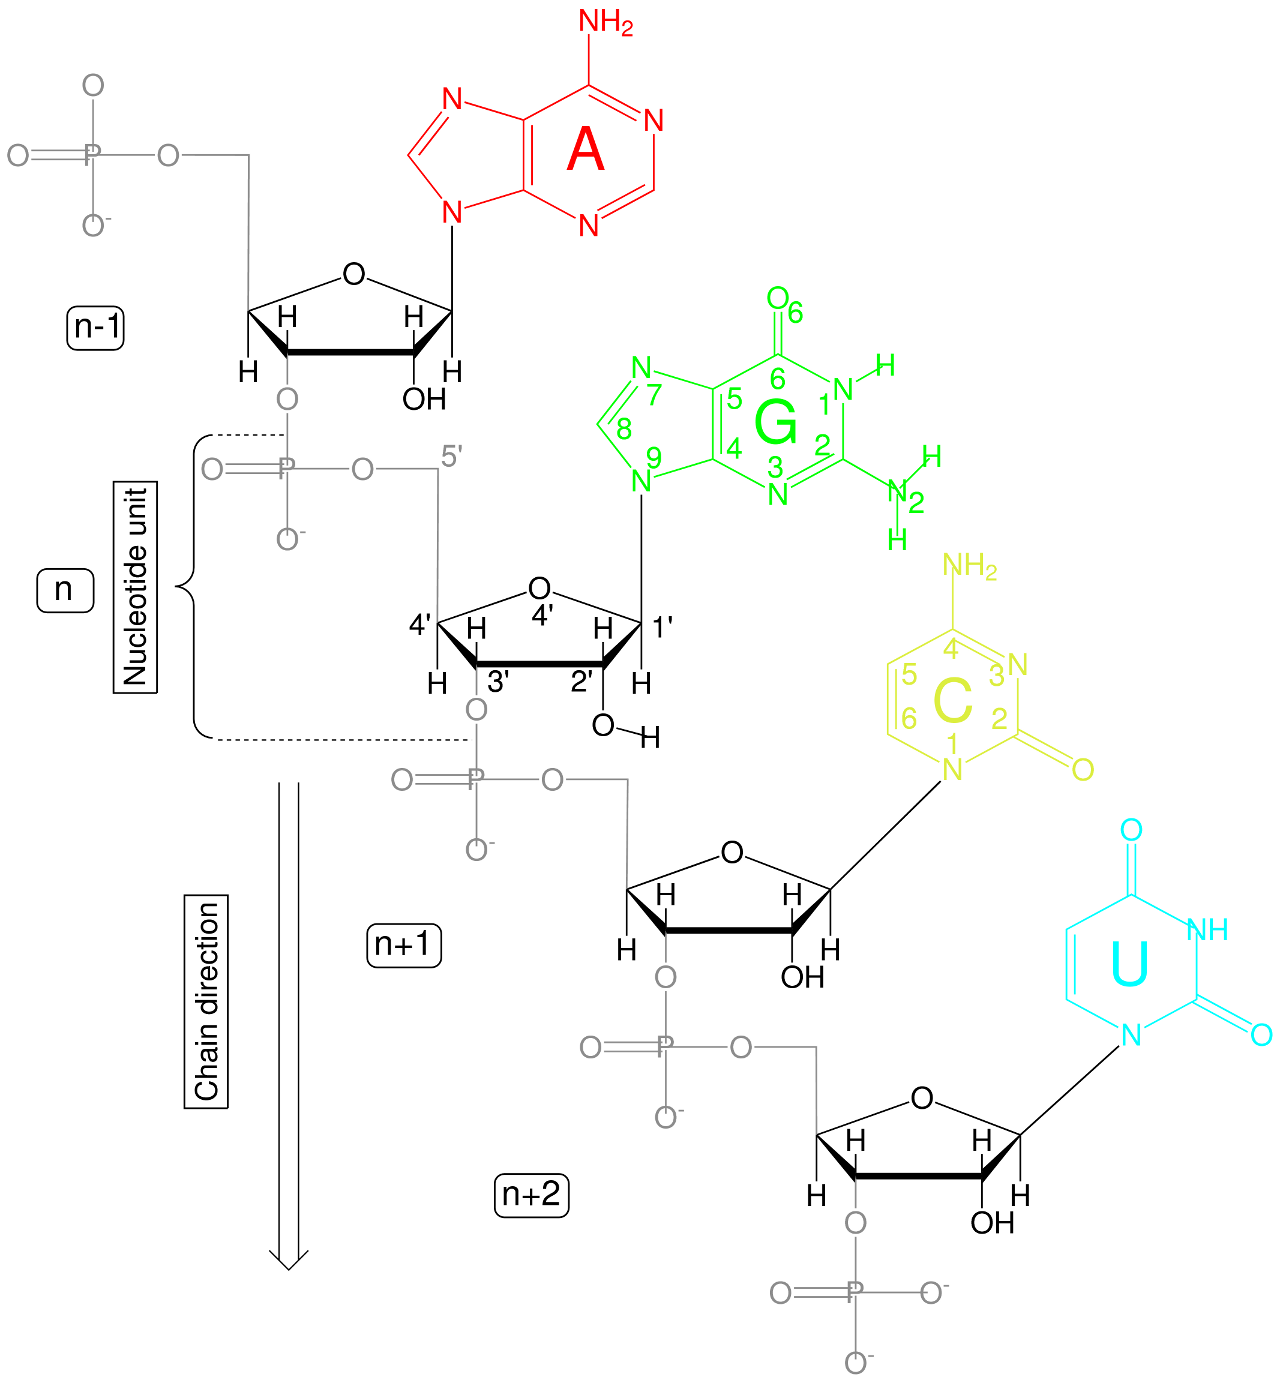
\includegraphics[scale=3.0]{Chapter1/chemistry1b.png}
\caption{A  single strand  of  RNA drawn  in  the 5$'$  to 3$'$  sense
  showing the  main chemical entities  which compose it;  base, sugar,
  and backbone.  The four bases (A,  G, C, U) are colored according to
  the  NDB  (Nucleic  Acid  Database)  convention  \cite{ndburl},  the
  backbone is colored gray, and the  sugars black. The bases G, and C,
  and the  furanose sugar  are numbered according  to the  IUPAC rules
  \cite{iupac1983}. This  figure is a  reproduction of Figure  2.1, in
  Wolfram Saenger's book \cite{saenger1984}.}
\label{fig:chemistry1}
\end{figure}  

Heterocyclic bases can form a diversity of base-pairs through hydrogen
bonding and  can be classified in  28 classes as  suggested by Saenger
\cite{saenger1984},   and  as   seen   in  Figure~\ref{fig:saenger28}.
Nomenclatures which  conform to Saenger's classes  have been developed
by Lee-Gutell \cite{lee2004}, Leontis-Westhof \cite{leontis2002b}, and
Lemieux-Major \cite{lemieux2002}.

\begin{figure}
\centering
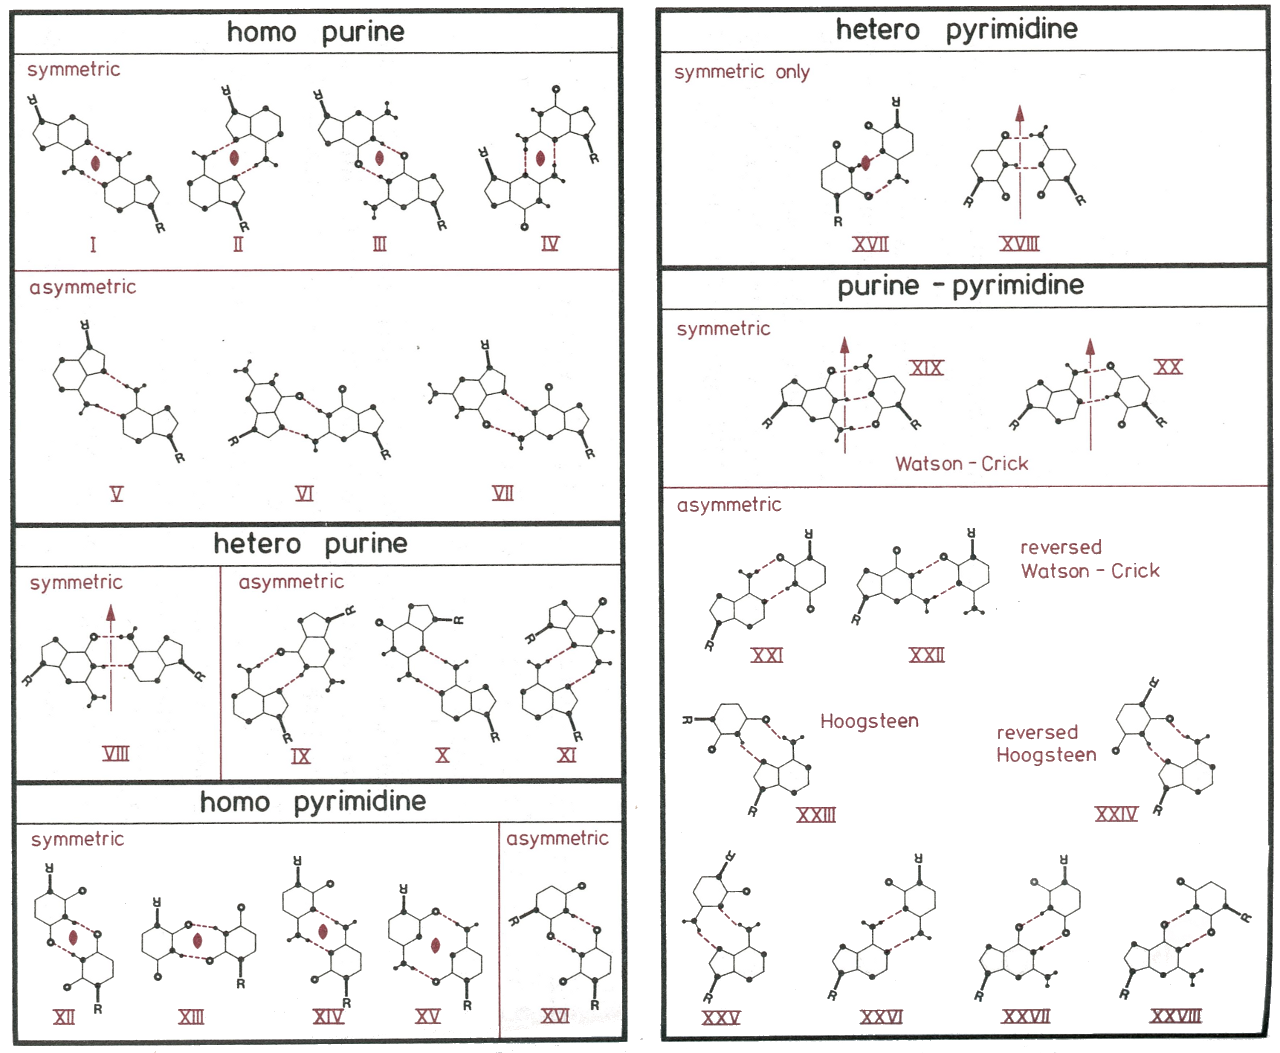
\includegraphics[scale=4.0, angle=90]{Chapter1/saenger28b.png}
\caption{Saenger  base-pairing  classes,  reproduced  from  his  book,
  "Principles of Nucleic Acid Structure". \cite{saenger1984}.}
\label{fig:saenger28}
\end{figure}  

The other non-covalent interactions which are common to the nucleotide
bases  are those  of  stacking through  London  dispersion forces  and
electrostatic  interactions.   It  has  been hypothesized  that  $\pi$
electron  interactions  could  also  account for  stacking,  but  very
precise quantum calculations \cite{sponer1996, sponer1997} have show
otherwise thus far.

Sugar, and  backbone can adopt a variety  of conformations constrained
to the values of their torsion  angles. In the case of the sugar these
torsion angles are called puckers,  perhaps in analogy to the gestures
made  by human  lips.   The prefered  sugar  pucker in  RNA is  called
C$_{3'-\textrm{endo}}$,  but in  cases where  an intercalated  base is
acommodated between two sequential  bases, the sugar pucker changes to
a non-prefered  conformation called C$_{2'-\textrm{endo}}$.  Standards
to  describe the  conformations resulting  from the  specific  sets of
torsion angle  values which sugars  and backbone can attain  have been
developed and can be seen  in textbooks \cite{saenger1984}, in the web
\cite{jenaurl}, and in  the IUPAC recommendations \cite{iupac1983}. We
refer the reader to these sources for a more detailed description, and
limit  ourselves  to  show  in Figure~\ref{fig:puckersbbone}  a  brief
description of these torsion angles.

\begin{figure}
\centering
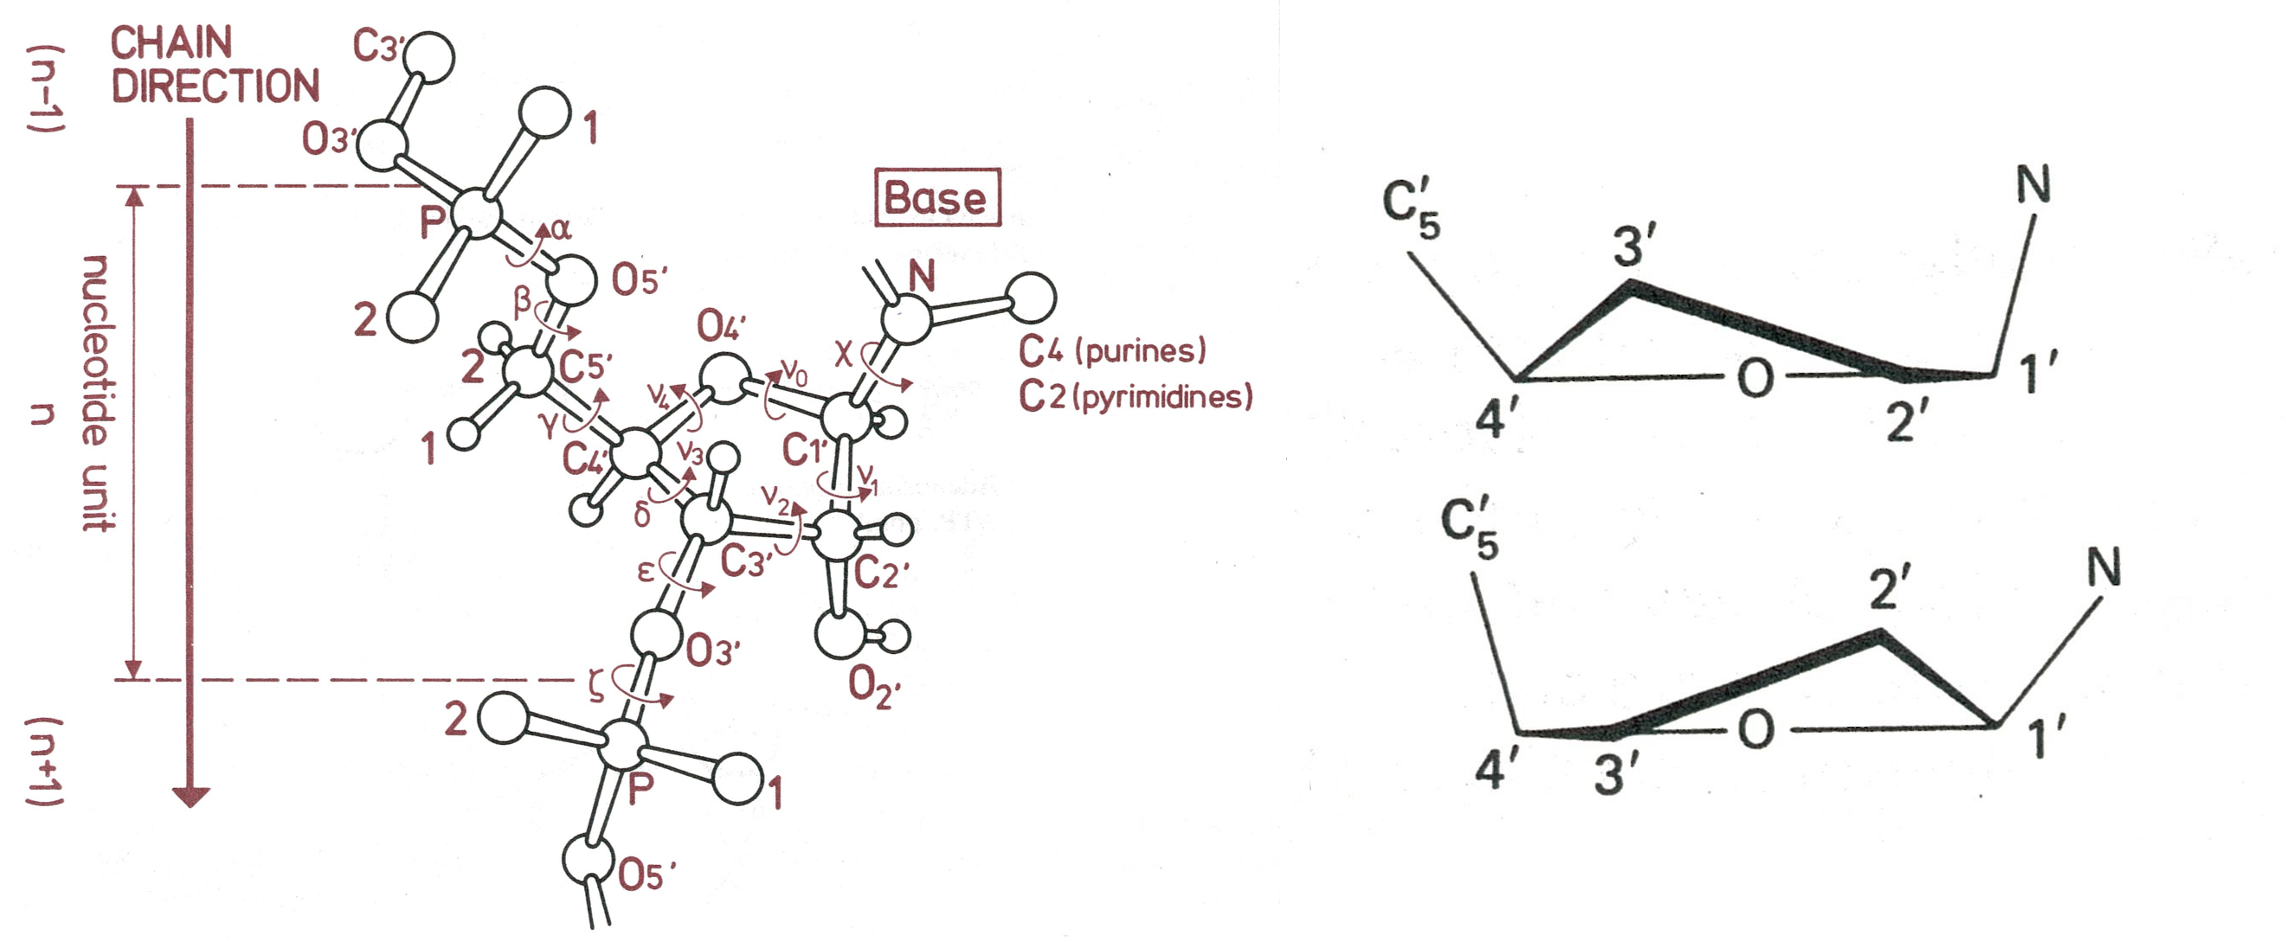
\includegraphics[scale=1.8, angle=0]{Chapter1/torsions.png}
\caption{\textbf{Left:}      Backbone      and      Sugar      torsion
  angles. \textbf{Right:}  The most common  sugar pucker conformations
  in  RNA,  that is,  C3'endo  and  C2'endo,  reproduced from  Wolfram
  Saenger's,         "Principles        of         Nucleic        Acid
  Structure". \cite{saenger1984}.}
\label{fig:puckersbbone}
\end{figure}  

%A-RNA 
%Loops
%Reference:
%Pure \& Appl. Chem., Vol.55, No.8, pp.1273—1280, 1983
%\url{http://www.fli-leibniz.de/ImgLibDoc/nana/IMAGE_NANA.html}


\section{RNA folding}
The first  high-resolution X-ray\index{X-ray} structure  of RNA larger
than a dinucleotide was  that of yeast tRNA$^{\textrm{Phe}}$ at 3{\AA}
in  1974 \cite{robertus1974,  kim1974, stout1976}.   Thirty  six years
later there  are two orders  of magnitude more  structural information
about RNA \cite{noller2005}, and new information from non-coding RNA's
is  expected  \cite{weinberg2009}.  This  fact  and  the discovery  of
ribozymes  \cite{kruger1982,  takada1983},  which  are  catalytic  RNA
molecules, has  renewed interest in solving  the RNA folding\index{RNA
  folding}  problem,  that is,  starting  from  the primary  sequence,
finding in  an automated\footnote{The term  automated is used  here to
  mean  a  theoretical model  of  tertiary  folding,  which could  use
  experimental measures of secondary structure association in the same
  way   that  the  traditional   secondary  structure   folding  model
  \cite{zuker1989,    hofacker1994}    uses    the    Tinoco-Uhlenbeck
  dinucleotide   postulate  \cite{borer1974}   to   find  total   free
  energies.}   way the  native three-dimensional  structure of  an RNA
molecule  and   the  folding  pathway   that  it  follows.    The  RNA
folding\index{RNA folding} problem is usually seen as analogous to the
protein folding  problem, due both  to the discovery of  the enzymatic
behavior  of  RNA \cite{kruger1982,  takada1983}  and the  complicated
folding of large RNA molecules \cite{batey1999}.  To take advantage of
this analogy,  a unified conceptual  framework for describing  RNA and
protein folding, called the  kinetic partitioning mechanism (KPM), has
been developed by Thirumalai and Hyeon \cite{thirumalai2005}. This and
other methods are based on defining an adequate partition function for
describing  the correct conformational  ensemble of  folded, partially
folded,    and   unfolded    structures    \cite{chen1995,   chen1998,
  thirumalai1996} of either protein or RNA.

\section{Is RNA folding a hard or easy problem?}
There  are  two trains  of  thought  regarding  the mechanism  of  RNA
folding.  One  states that  RNA folding is  less complex  than protein
folding  \cite{tinoco1999} because  RNA is  made up  of a  four letter
alphabet of similar  nucleotide units instead of a  20 letter alphabet
of  dissimilar   amino  acids.   Therefore  the   number  of  possible
sequential  combinations  is smaller.   It  is  also  well known  that
secondary and  tertiary interactions can  be separated in the  case of
RNA  by the absence  or presence  of Mg$^{2+}$  \cite{rangan2003} (see
Figure~\ref{fig:folding}), and  that the secondary structure motifs
of RNA are more limited  in  number  than  those  of protein,  whereas
secondary  and tertiary elements are not as easily separable in
proteins.
\begin{figure}[ht]
\centering
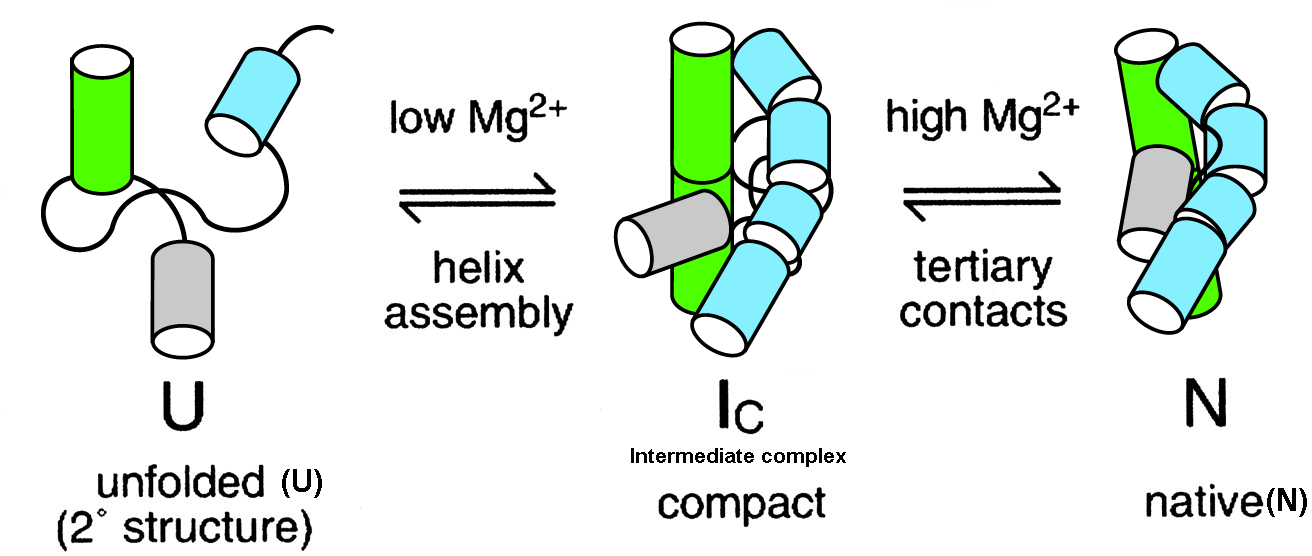
\includegraphics[scale=0.3]{Chapter1/rangan2003pnas.png}
\caption{Separation  of  secondary  and  tertiary interaction  in  RNA
  \cite{rangan2003}. Double helical secondary structure represented by
  individual  cylinders and  tertiary interactions  by  association of
  cylinders. Color coding stands for separate  helical regions of
  RNA, and the connecting  black strings represent single stranded loop
  structures.}
%% Note that Dr. Olson asks what the colors in cylinders mean.
%% Answer: They mean nothing. Perhaps only that the cyan stands for
%% the helical structures making a pseudo-knot, that is, P7 and P3.
\label{fig:folding}
\end{figure}
The  other point of  view says  that RNA  folding can  be at  least as
complex as protein folding \cite{moore1999a, sorin2004} since there is
no such thing  as hydrophobic burial of regions of RNA  as in the case
of  proteins.   Instead, the  electrostatic  problem  stemming from  a
complex charged backbone must be dealt with in the case of RNA.
% The case of the electrostatic treatment of the backbone is lacking
% here, most likely WKO wants me not to ignore our own Gerald Manning
% tinoco 1999 says this must be an easy to solve problem since we can
% do the electrostatics for it easily
For instance,  the interactions of  the RNA polyanionic  backbone with
water  and cations  \cite{klein2004a}  are not  easily simulated  with
explicit   solvent  models   like those used to treat   proteins.  The
aforementioned interactions of RNA  need to be modeled implicitly, and
must aim to describe long dynamic processes of the order of seconds to
minutes,  in  contrast   to  the  typical  time  scales   of  tens  of
microseconds associated with protein folding.
% Remember that this means that a explicit calculation for RNA would
% be prohibitively large.

Although   secondary   and  tertiary   structure   can  be   separated
experimentally, there have been few theoretical efforts to account for
the  folding  of  RNA  from  a random  sequence  of  nucleotides  into
secondary structures and tertiary  structures. What little is know has
been  investigated at  low resolution.  Stephen Harvey  and associates
have   simulated   the   folding   of   yeast   tRNA$^{\textrm{Phe}}$,
\cite{malhotra1990}  and  the  assembly  of  the 30S  subunit  of  the
ribosome \cite{stagg2003} at various levels of detail, initially using
only one pseudoatom  per helical region, and later  one pseudoatom per
nucleotide.  Recently  Fran\c{c}ois  Major's  group  at  Montreal  has
proposed a pipeline of two  computer algorithms to study RNA structure
\cite{parisien2008}.   One    pipeline   makes   secondary   structure
predictions, and the  other assembles 3D structures based  on the best
scoring secondary structures.
% Note for presentation ==> Include figure 1 in Malhotra-harvey paper
% Look at what says in folding.stanford.edu/science.html Also take
% into account Biophys J. V.88 2516-2524 for the case of having to
% think of water in the folding problem.
By contrast,  in the case of  proteins many groups  have simulated the
transition  from  secondary  to  tertiary  structure,  including  some
calculations which  account for the  strong coupling of  secondary and
tertiary  structure   \cite{westhead1999,  gerstein2003,  meiler2003}.
This type of work is  often referred to as protein structural topology
and there is no counterpart for RNA.

%The seminal paper here seems to be the one of liphardt in 2001 for
%rna unfolding
\section{Experimental folding techniques}
Traditionally   RNA   folding  and   unfolding   have  been   followed
calorimetrically  and spectroscopically as  a function  of temperature
and cation concentration  \cite{bloomfield2000, boots2008}. While this
approach  works well  for studying  two-state  folders, \textit{i.e.},
structures  which populate  only two  states (native  and  melted), in
general RNA's  are not  two-state folders. RNA  seems to go  through a
rugged  free  energy landscape  of  conformations  in  the process  of
folding \cite{zhuang2003}.  The  experimental solution to this problem
is offered  by single-molecule techniques  like fluorescence resonance
energy transfer (FRET) and  mechanical micromanipulation, in which the
ends of RNA  are attached to micron sized beads  which are then pulled
apart  and  monitored  with  a laser  light  trap  \cite{liphardt2001,
  onoa2004,  tinoco2004, hyeon2005}.  In  the case  of single-molecule
force-induced   unfolding,  state   transitions   often  occur   under
non-equilibrium  conditions, thereby  making it  difficult  to extract
equilibrium  information from the  data. Bustamante, Tinoco,
and associates have shown that by using the Crooks fluctuation theorem
\cite{crooks1999},  one  can deal  with  such  cases  and extract  RNA
folding    free     energies    from    single-molecule    experiments
\cite{collin2005}. Recently an alternative solution to this problem has
been proposed by Thirumalai and associates based on single-molecule
force-quenching experiments, by using a so called  de Genes "expanding
sausage model" \cite{hyeon2009}.
%\subsection{RNA Folding in Vitro vs in Vivo vs in Silico}
% It still is to be seen whether the following is relevant or not
% This single molecule information is
% collected in-vitro and not in-vivo, which is actually the ultimate
% problem aimed for prediction, there's quite a lot of evidence for
% different folding states reached in one case and not the other and
% viceversa \cite{sosnick2003, schroeder2002} but still a first step
% towards understanding in-vivo folding is in-vitro and in-silico
% experimentation.


\section{RNA simulations}
Network  and molecular  mechanics-molecular  dynamics (MM-MD)  methods
provide  useful  information  relevant  to the  RNA  folding-unfolding
problem, especially  for describing fluctuations away  from the native
conformation.   Gaussian network  models  \cite{y_wang2004, bahar1998,
  wang2005}, which  treat RNA  at less than  atomic detail,  have been
used  to  describe  the  motions  of large  RNA  structures  like  the
ribosome.  Examples  of the  predicted normal modes  of motion  of the
ribosome  can be  seen at:  http://ribosome.bb.iastate.edu/70SnK mode.
Using MM, Sanbonmatsu and coworkers  obtained a static atomic model of
the    70S    ribosome    structure    through    homology    modeling
\cite{tung2004}.  Tung  and  associates  used this  structure  for  an
all-atom  MD simulation  of the  movement of  tRNA into  a fluctuating
ribosome  \cite{sanbonmatsu2005}.  This  type of  simulation  might be
useful in a  reverse-folding approach to the RNA  folding problem.  To
the best of our knowledge,  such calculations haven't as yet been done
for RNA.

\subsection{Local nucleotide interactions}
%\subsubsection{QM approaches and MM consequences}
The molecular  interactions that  rule  RNA structures at  the nucleic
acid base level, \textit{i.e.},  local level, are hydrogen bonding and
stacking interactions. The former are  related to base pairing and the
latter, in most cases, to  nucleotide steps. These interactions can be
explored  theoretically at various  levels. At  the highest  level are
ab-initio  quantum   mechanical  calculations  which   are  still  too
expensive   for  systems  as   large  as   hundreds  of   atoms.  Such
calculations,  nevertheless,  can  tell   a  great  deal  about  local
electronic behavior.  For example, Hobza and  collaborators have found
that the  stacking interaction of free nucleotide  bases is determined
by   dispersion  attraction,   short-range  exchange   repulsion,  and
electrostatic  interaction.  No  specific $\pi-\pi$  interactions  are
found     from    electron    correlated     ab-initio    calculations
\cite{sponer1996, sponer1997}.  This is  why force field  methods have
been so successful in the  study of nucleic acids, since the empirical
potentials used  in such studies  mimic well the  quantum mechanically
obtained energy profiles \cite{tung2004, sponer2000}.
% since they can be modeled easily with simple empirical potentials
% consisting of Lennard-Jones, van der Waals and Coulomb terms.
% What the recent results say it's simply that by using a larger
% basis set, they can account for some interactions which were not
% included before, and maybe because of taking better account of
% electron-correlation.
A currently debated ab-initio finding is whether small fluctuations in
the   configurations   of   neighboring   base  pairs   (dimers)   are
iso-energetic  or  not.   Recent  calculations  of  Sponer  and  Hobza
\cite{sponer2006}    seem   to    contradict   their    earlier   work
\cite{sponer2000,  hobza2002},  in which  the  stacking energies  were
reported to  be relatively insensitive to dimer  conformation. The new
results  use  the so-called  ``coupled  cluster  singles doubles  with
triple electron excitations'' CCSD(T)  method, to account for electron
correlation.  Using  this electron correlation  energy correction, the
stacking energy differences between dimer conformations turn out to be
considerably higher than previously reported.

% therefore justifying rigid body parameter interpretations.
% \subsubsection{Experimental Stacking and Polyionic backbone}
Single-strand and double-strand stacking free energies can be obtained
calorimetrically \cite{freier1985}.   One of the  most popular methods
used   for  obtaining   such  quantities   is   differential  scanning
calorimetry (DSC) \cite{marky1982}.  These measurements show favorable
dinucleotide stacking  free energies as  large as $-3.6$  kcal/mol for
double-strand  stacking.   Experimentally,  the  magnitudes  of  these
interactions      are     found      to      be     sequence-dependent
\cite{bloomfield2000}. In  fact, the  stacking free energies  for some
sequences\footnote{Free   Energies   for   5'   unpaired   nucleotides
  (e.g. UC/A  UU/A) are quite small  (i.e.  $<$ 0.4  kcal/mol) and are
  termed  weakly stacking bases.\cite{burkard1999,  burkard1999b}} are
found to  be negligible.   Thus there may  be no  accountable stacking
interaction at all for some sequences.

Besides  taking into  account  the effects  of  stacking and  hydrogen
bonding,  it  is  important  to  think  at the  same  time  about  the
polyelectrolyte  nature  of the  RNA  backbone.  Manning's  counterion
condensation theory \cite{manning1977,  manning2003} provides a simple
and   quantitative  picture   of   the  interactions   of  a   regular
double-helical  nucleic acid  polyanion with  its counterions,  but it
does   not  take   into  account   the  discrete   nature   of  charge
\cite{bloomfield2000} or the  folding of RNA. Poisson-Boltzmann theory
offers a more detailed picture of the behavior of charged macroions in
solution \cite{antypov2005, xu2007}.
% Talk more about counterion condensation, thirumalai discusses it on
% his 2001 paper also chapter 8 of Bloomfield, Crothers, Tinoco
% (References \cite{manning2003} Ray-Manning?).
% Real Experiments results for stacking energies and polyanion
% energies and Energetics related to cation metal presence
% WKO says that there might be old experimental data that are contrary
% to this and that I must show it here, so far what I've found is
% Saenger saying that based on old QC and this is different, he
% relates it to hydrophobicity concepts. Talk about experiments.

The local conformational  space of RNA has been  studied using a large
set of available  RNA structures from the Nucleic  Acid Database (NDB)
\cite{berman1992}.  The  torsion angles  of the nucleotide  steps have
been   clustered    using   different   techniques   \cite{murray2003,
  schneider2004}.   The  root-mean-square  deviations  (RMSD)  of  the
distances between closely spaced  atoms in the phosphates, sugars, and
bases, have  also been clustered \cite{sykes2005}.  The latter studies
are aimed  at finding the  common nucleotide base steps  and base-pair
building  blocks which  have  been  given the  name  of RNA  doublets.
Recently, the  RNA Ontology Consortium (ROC) has  proposed a consensus
set  of RNA dinucleotide  conformers integrating  the work  of various
groups \cite{richardson2008}.


\subsection{RNA  secondary  structure   algorithms  and  the  lack  of
 tertiary ones}
From   secondary   structure   prediction  algorithms   like   Zuker's
\textit{mfold} program \cite{zuker2003}, Hofacker's Vienna RNA package
\cite{hofacker1994}, or  Mathews Dynaling software \cite{mathews2002},
one obtains  a large ensemble  of secondary structure graphs,  i.e. 2D
representations of  the double-stranded helical  stems, hairpin loops,
bubbles formed by the constituent bases.  These graphs can be analyzed
with graph  theory to produce  a partition function describing  a full
arrangement  of contacts for  the total  number of  possible secondary
structures, allowing  the construction  of a "relation  of microscopic
conformations to macroscopic  properties" \cite{chen2000}. So far this
type of model  has not been generalized to  take into account tertiary
structural features, \textit{i.e.},  interhelical interactions of RNA.
In  the  last  two to  three  years  a  boom  in prediction  of  small
($\approx$ 200  nucleotides) RNA 3D structures  has started. Basically
three types of approaches are being  followed.  One is that of using a
coarse-grained model, assigning a potential function to it, applying a
minimization procedure, and then performing a molecular mechanics (MM)
all-atom  refinement \cite{das2007,  ding2008,  jonikas2009a}. Another
starts  from  the predicted  secondary  structures,  assumes that  the
helical  regions adopt  the canonical  A-form  structure, mechanically
inserts residues as rigid bodies in the remaining non-helical regions,
and  finally carry  out an  MM optimization  \cite{martinez2008}.  The
third  approach   entails  a  pipeline   between  secondary  structure
prediction, and tertiary structure assembly is proposed. This pipeline
uses  as bridging  concept  between  2D and  3D  structure, the  graph
theoretical definition of a minimum cycle basis, which for the case of
nucleic  acids  has  been  renamed  as  Nucleic  Cyclic  Motifs  (NCM)
\cite{parisien2008}.

\subsection{RNA  overall fold}
Whereas  in  the case  of  proteins  one  qualitatively describes  the
overall  fold  in terms  of  the  arrangement  of secondary  structure
motifs, \textit{i.e.}, using the helix-ribbon-coil images developed by
Jane           Richardson          \cite{richardson2000}          (see
Figure~\ref{fig:ribboncoil}), there is still no comparable description
of  the overall  fold of  RNA. A  ribbon representation  of  the sugar
phosphate backbone (see Figure~\ref{fig:ribosome}) helps to understand
the  folding of  small  RNA's, but  in  the case  of  the ribosome,  a
representation at such level of detail does not allow to make sense of
such  a large  structure  (close  to 3000  nucleotides  for the  large
subunit of  the archaeal  ribosome).  In the  past two  years Holbrook
\cite{holbrook2008}  and  Sykes  \cite{sykes2009}  have  proposed  new
representations for RNA based on helical region organization. Holbrook
makes  an  analysis of  continuous  interhelical  strands, so  called,
COINS, and Sykes makes an optmized projection of 3D helical axis to 2D
images,  which can  later  be annotated  with,  for example,  hydroxil
radical footprinting results.

\begin{figure}[ht]
\centering
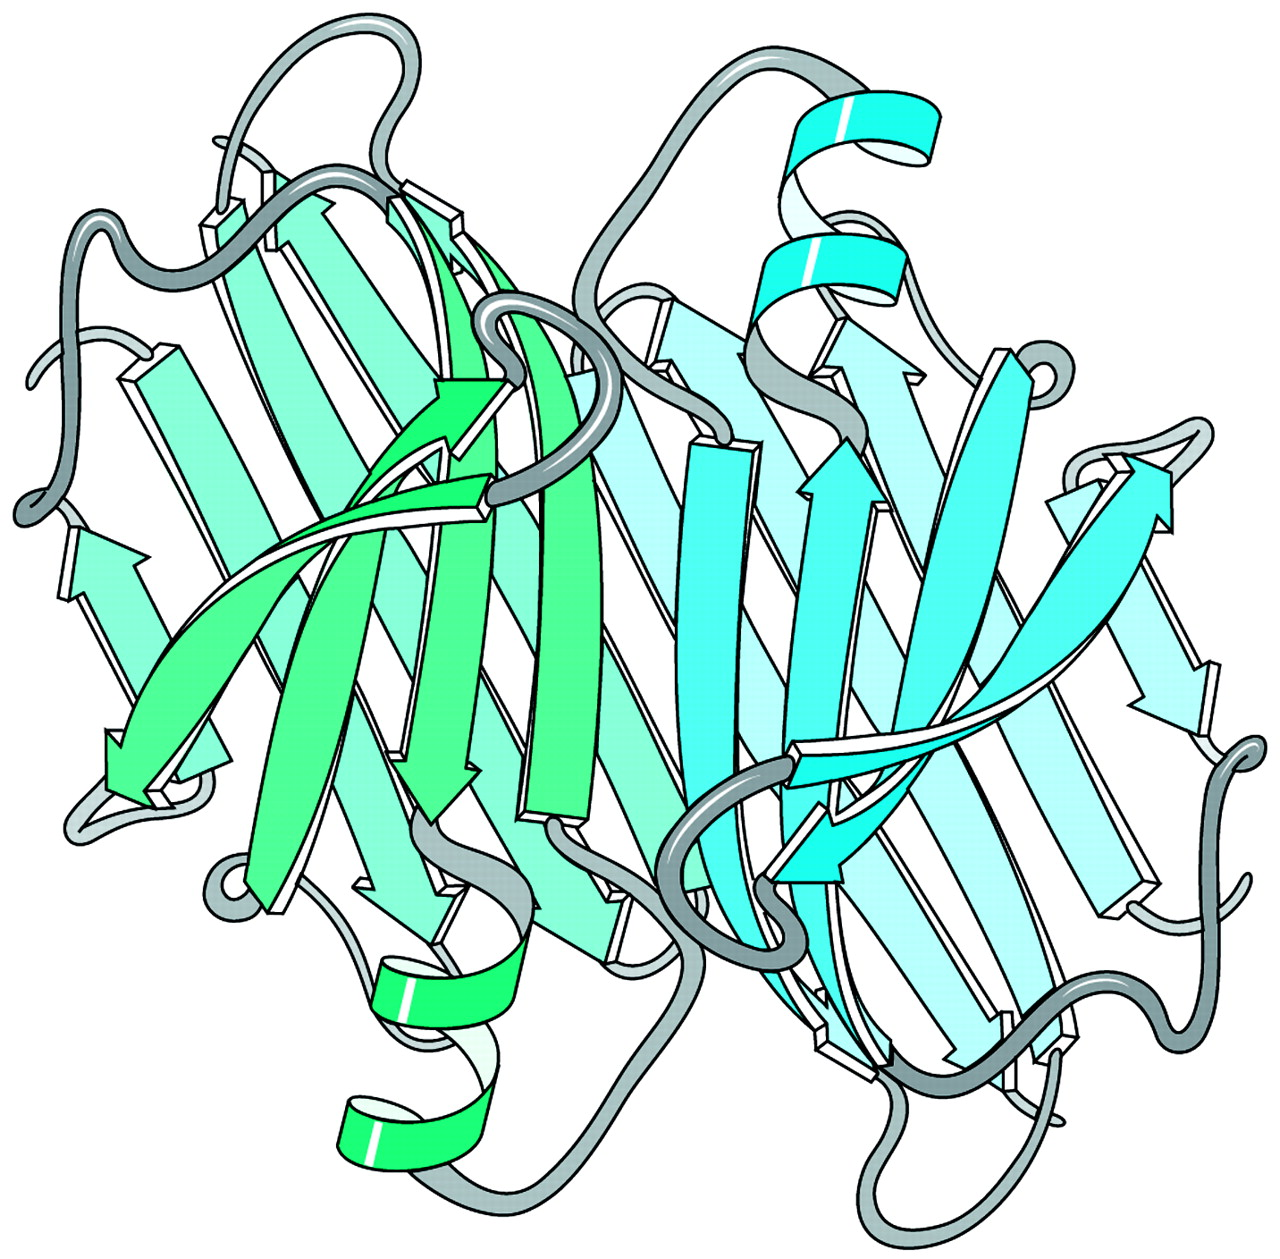
\includegraphics[scale=0.4]{Chapter1/overallfold.png}
\caption{Ribbon-coil    schematic    illustraring    the   fold    and
  intermolecular  units of  a dimer  of prealbumin  (PDB\_ID:2pab), or
  transthyretin,    taken     from    Richardson    \textit{et    al.}
  \cite{richardson2002}}
\label{fig:ribboncoil}
\end{figure}

\begin{figure}[t]
\centering
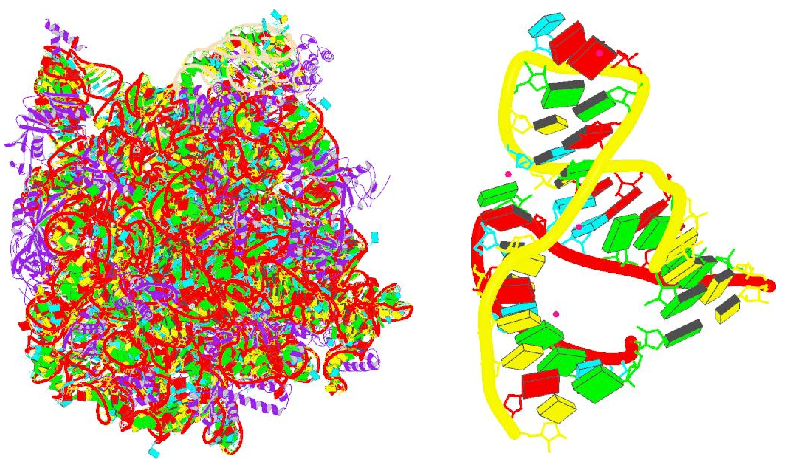
\includegraphics[scale=0.5]{Chapter1/ribosome_ribozyme.png}
\caption{Images   of  the  \textit{Haloharcula   marismortui's}  large
  ribosomal subunit NDB\_ID:RR0033 (left) and the hammerhead ribozyme
  (right) NDB\_ID:UR0029.
  The  figures were taken directly  from the NDB
  web  pages,   and  show  a  3DNA   generated  \cite{lu2008b}  ribbon
  representation of the phosphate backbone, and a block representation
  for the nucleotide bases. From  the figures it's clear that, whereas
  the   ribozyme   fold   can   be  clearly   understood   with   this
  representation, the ribosome fold cannot.}
\label{fig:ribosome}
\end{figure}

One  can  envision that  a  thorough  investigation  of the  space  of
translational and rotational degrees of freedom of the helical regions
of RNA could give clues as to  how we might see an overall fold in RNA
structures.  To the  best  of  our knowledge  there  is no  comparable
quantitative description of the folding of proteins.

In  the  case  of  proteins  the SCOP  (Structural  Classification  of
Proteins)  database  \cite{andreeva2004},  classifies proteins,  among
various  qualitative  descriptors,   according  to  folds,  which  are
recurrent  arrangements of  secondary structure,  that is,  a  list of
secondary  structures with  unique topological  connections.  The SCOR
(Structural  Classification  of  RNA)  database  \cite{klosterman2002,
  klosterman2004}, aims  to provide  a similar classification  to that
obtained   for  proteins,   but   using  RNA   motifs  instead.   This
classification focuses on the local folding of small pieces of RNA and
cannot  describe  the  overall  fold.  Local  classification  is  also
qualitative rather than quantitative.

\subsection{RNA motifs}
The term ``\textit{RNA motif}'' is  used in the literature to describe
three   different   levels    of   RNA   organization,   namely,   RNA
\textbf{sequence} motifs, RNA  \textbf{secondary structure} motifs, or
RNA \textbf{3D structure} motifs.   Because these distinctions are not
always clearly made the beginner may result in confused and frustrated
bibliographical searches.

The lack of a unique definition of RNA motifs is yet another source of
confusion  in  understading  RNA  motifs  is  the  lack  of  a  unique
definition.  Three  popular and  somewhat  recent  definitions of  RNA
motifs include:
\begin{itemize}
\item{``\textit{a discrete sequence or combination of
    base  juxtapositions   found  in  naturally   occurring  RNA's  in
    unexpectedly high abundance.}''\cite{moore1999}}
\item{``\textit{conserved structural subunits that make
    up the secondary structures of RNAs.}''\cite{holbrook2005}}
\item{``\textit{ordered   stacked    arrays   of
    non-Watson-Crick  base  pairs  that  form distinct  folds  on  the
    phosphodiester backbones of RNA strands.}''\cite{leontis2003}}
\end{itemize}

The  kind of RNA  motifs addressed in this
thesis are of the third type, that is, RNA \textbf{3D structure}
motifs  which we henceforth term RNA  motifs.
From our point of view RNA motifs are to be understood as  peculiar
sets of geometrical  (in the rigid block sense)  arrangements in
three-dimensional space.

Even  though there  is no  unique definition,  we can  think  of three
practical  tasks regarding  RNA  motifs.   That is,  given  an RNA  3D
structure automatically identify, describe,  and find new motifs.  For
automatic  identification of  RNA motifs  Pyle and  collaborators have
developed  a software called  AMIGOS. This  software finds  RNA motifs
based on  specific values of backbone virtual  torsion angles $\eta$
and  $\theta$  \cite{olson1980, malathi1985,  duarte2003} in  a  way  which
resembles   a   Ramachandran  plot   analysis.    Lemieux  and   Major
\cite{lemieux2006}  provide  the  software MC-Fold,  which  implicitly
finds RNA motifs based on  an algorithm to determine so called nucleic
cyclic  motifs, which  are  just the  minimal  cycle basis  of an  RNA
secondary  structure  interpreted as  a  mathematical graph.   Leontis
\cite{nasalean2009}  and collaborators  provide FR3D  (read  as FRED).
F3RD is  a matlab  windows executable program  which finds  RNA motifs
based on the isostericity matrices of base-pairs.

For description of RNA motifs Schlick and collaborators have used FR3D
to  localize  RNA helical  junctions  of  order  four (i.e.   four-way
junctions) or  higher, and performed a  visual analysis to  see if the
helices  in  such junctions  form  coaxial  stacks  or not,  and  have
classified   them   accordingly   \cite{laing2009,  laing2009a}.    As
mentioned previously in the context of RNA folds, Holbrook, and Sykes,
describe   helical  regions  and   display  them   in  two-dimensional
representations. Sponer's group has carried out the description of RNA
motifs present  in the ribosome using Molecular  Dynamics (MD) methods
implemented  in   the  AMBER   package.   They  have   performed  25ns
simulations  of   the  Sarcin-Ricin  Domain  (SRD)   of  the  ribosome
\cite{spackova2006}, and also 80ns  simulations of hydration of loop E
in the 5S subunit of the ribosome \cite{reblova2003}.

The software programs which perform the task of identifying RNA motifs
in RNA structures also have the ability to find new RNA motifs, as is
the case for AMIGOS, MC-Fold, and FR3D.

\section{Overview}
Keeping always in  mind the greater scope of  the RNA folding problem,
this thesis  addresses various issues of  RNA structural understanding
using RNA crystallographic data from the Protein Data Bank (PDB). Such
data  has been  analyzed statistically  in terms  of a rigourous
rigid-body formalism.  In Chapter 2 the consensus clustering technique
is   used  to   classify   RNA  base-step   parameters  of   non-A-RNA
conformations, and  the resulting groups are  localized and understood
in the context  of rRNA.  Chapter 3 reconsiders  previous work carried
out by  Dr. Yurong Xin  at the Olson's  lab, on classification  of RNA
base-pairs by  resorting again to clustering  analysis techniques, and
database  mining  of the  WWW  available  Base  Pair Structures  (BPS)
database.  In  Chapter 4 we  explore, using statistical  analysis, the
data available  on RNA  helical regions, and  use this  information to
compute the persistence length of double-stranded RNA's and compare it
to  experimental  results.  In  Chapter  5 we  provide  a  new  python
software,  pyRNAmotifs which interfaces  with 3DNA  to do  a rigourous
search of existing and perhaps  new RNA motifs, and finally in Chapter
6  we propose  the measurement  and classification  of  RNA structures
using a  new graph theoretical index  named folding index,  based on a
helical region "view"  of RNA's, which is clearly  concordant with the
emerging  necessity   of  new  metrics  beyond   RMSD  for  structural
understanding.

\bibliography{biblio}

    \chapter{Classification of  RNA Conformations}
%\bibliographystyle{abbvr}
%\bibliographystyle{nar}
\bibliographystyle{jacs}
\label{clustering} 

The problem of classification of the space of conformations
% configurations? 
of  RNA is  not new,  see  for example,  Olson 1972  \cite{olson1972},
Saenger     1984     \cite{saenger1984},     and    Gautheret     1993
\cite{gautheret1993}.  This problem  had  only been  addressed by  a few
researchers before the  turn of the twenty first century,  but starting in
the year 2000  a vast amount of RNA  structural information has become
available  with the  elucidation of  the  structure of  the 30S  small
ribosomal  subunit  of   \textit{Thermus  thermophilus},  a  bacterial
ribosome   \cite{wimberly2000,schluenzen2000},  and   the   50S  large
ribosomal subunit of \textit{Haloarcula marismortui}, an archaeal
\footnote{I emphasize the  phylogeny of rRNA's here since  there is an
  ongoing discussion among biologists on whether archaea are  closer
  to prokaryotes, or to eukaryotes.}  ribosome \cite{ban2000}.

\begin{figure}[H]
\centering
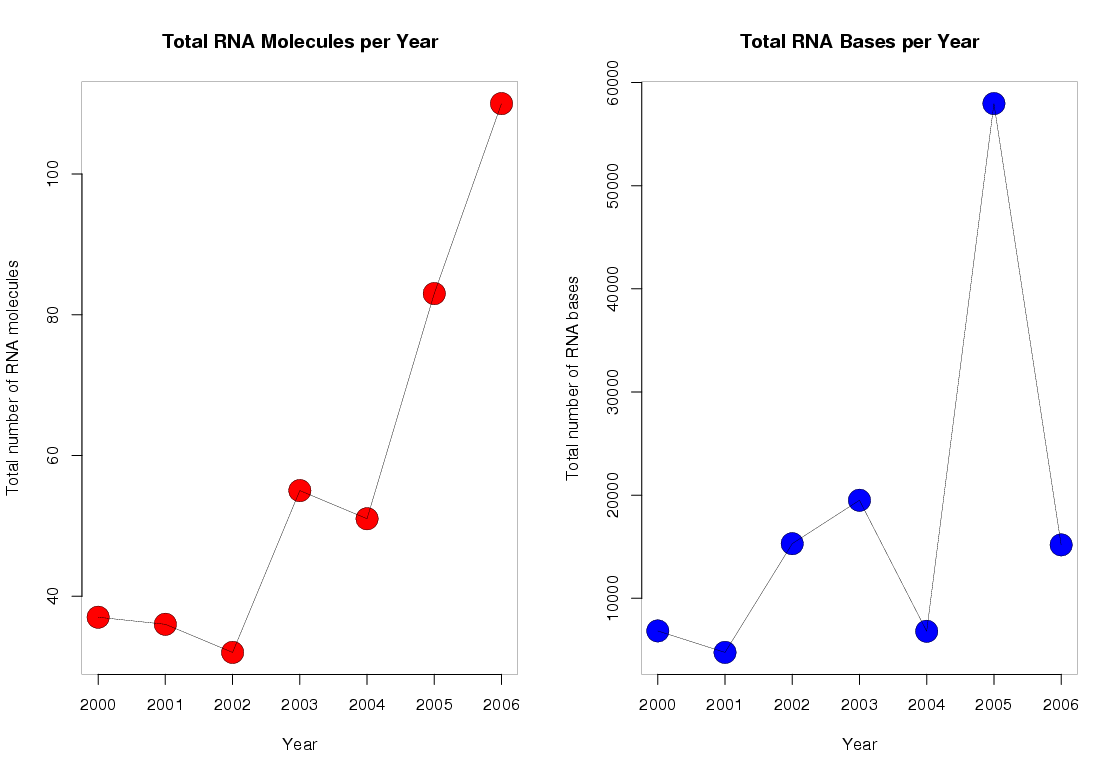
\includegraphics[scale=0.4]{Chapter1/rna_per_year.png}
\caption{\textbf{Left:} Total number of RNA structures solved yearly by X-Ray 
crystallography between 2000 and 2006. \textbf{Right:} Total number of 
RNA bases added to the PDB database between 2000 and 2006.}
\label{fig:rnainpdb}
\end{figure}

\noindent Between  1972 and  2000 a total  of 132 RNA  structures with
resolution greater  than 3 \AA, and comprising  around 5500 nucleotide
bases were found  in the Protein Data Bank (PDB),  and between 2000 and
today  a  total of  460  RNA\index{RNA}  structures comprising  around
140000  nucleotide   bases  have been  found.  That  is,   the  increase  in
information  due to  the solution of large RNA  structures  is two orders  of
magnitude as pointed out  by Noller \cite{noller2005} in 2005. Looking
at the growth of RNA structural information from 2000 until today it's
important  to  point  out  that,  although the  total  number  of  RNA
structures  deposited in the  PDB shows  exponential growth  (see left
panel in  Figure~\ref{fig:rnainpdb}), the total number  of RNA bases 
does not show a well defined trend (see right panel in
Figure~\ref{fig:rnainpdb}). 
This is due to the
size preponderance of ribosomal  structures. That is, in 2005 nineteen
ribosomal structures were  deposited in the PDB, whereas  in 2006 only
four  were deposited.  So, even  though interest  in RNA  seems  to be
growing  since  ribosomal structures  have become  available  in 2000,  and
two Nobel  prizes were awarded for work in  RNA in 2006, along
with  the  exciting  possibilities  of  deciphering  even  larger  RNA
virus\index{virus} structures, still the  growth of the RNA structural
field is  far from that  of proteins if  weighed by the growth  of RNA
structural information in  the past seven years. This  fact might just
be due to the smaller  sizes and structural diversity of RNA molecules,
which,  as can  be seen  in Figure~\ref{fig:rnaranges}, is  restricted  to
``compact'' nucleotide ranges\index{RNA!ranges}.
%\footnote{One can
% also think of another range of even larger viral RNA's \cite{heitsh}, and yet
%another one of nanodesgined RNA's \cite{shapiro, orland}}. 
A representative example of these  characteristic ranges can be seen in
Table 1.1 for structures larger than 300 bases.

\begin{figure}[H]
\centering
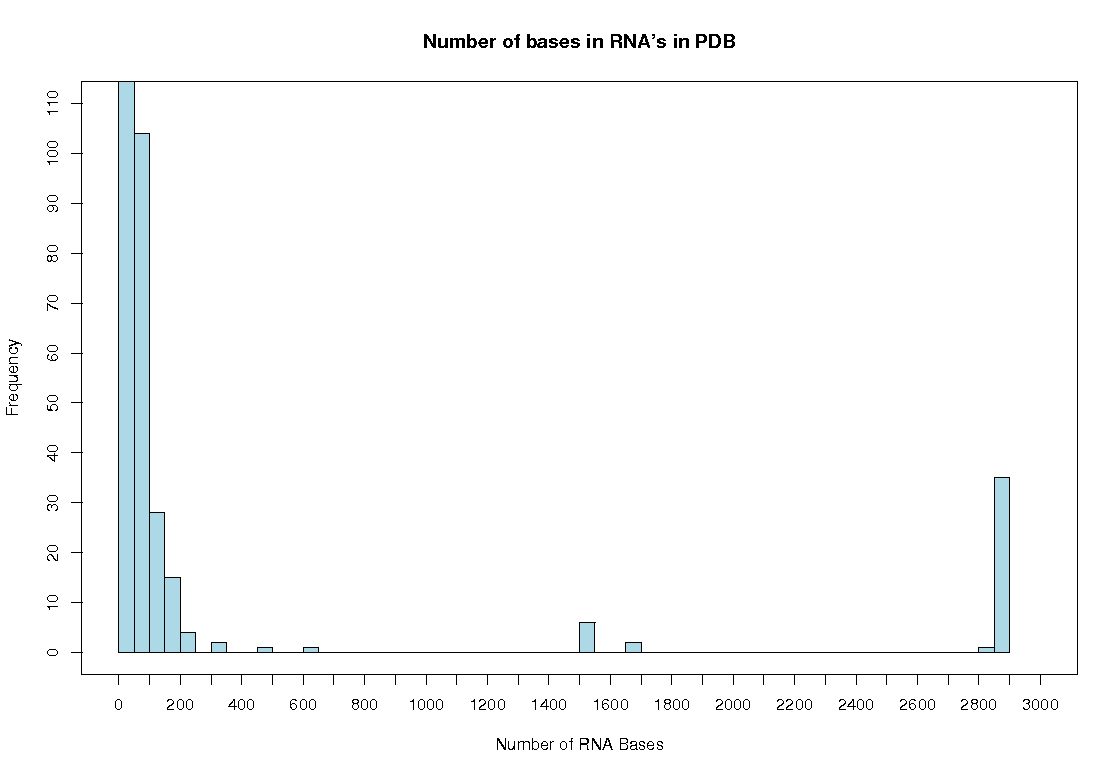
\includegraphics[scale=0.60]{histogram.png}
\caption{Frequency of nucleotide bases in RNA molecules found in the
  PDB classified by the size of RNA molecules. We define the size as the
  total number of nucleotide bases present per molecule.}
  \label{fig:rnaranges}
\end{figure}
%The table and Figure 1.1 come from downloading all structures from
%2000, until today that have RNA in the pdb and that have a resolution
%better that 3.0A, they are 460 structures.

\noindent Analysis of RNA conformational information contained in this
structural data can  be divided into three main  perspectives: an atom
based perspective; a bond  based perspective; and a third, as yet unexplored
to our knowledge,  rigid-body based perspective.   In the atom based
perspective,  either direct  comparison of  backbone atom  positions is
made \cite{reijmers2001}, or a comparison of distances between a reduced
set  of atoms  taken from  the  nucleotide backbone,  sugar, and  base
\cite{sykes2005}. The bond based  perspective is divided into three main
categories; the first considers the consecutive covalent bonds in the RNA
backbone and the glycosidic bond between the sugar and base,  that is, six
backbone   torsion   angles   and   one   glycosidic   torsion   angle
\cite{reijmers2001,  murray2003, hershkovitz2003, schneider2004,
hershkovitz2006};
or alternatively the pseudo-bonds between consecutive
P and  C4$\prime$ atoms  and the resulting  pseudo-torsion angles  $\eta$ and
$\theta$  \cite{olson1972,  duarte1998,  duarte2003, wadley2007}.  The
third category considers the  networks of horizontal hydrogen bonding
patterns coming  from a definition  of interacting edge  boundaries in
the nucleotide bases  \cite{westhof2000, leontis2002, leontis2006}. In
this report we review one category of the bond based
perspective. Namely we review the  case where the covalent bonds
between backbone atoms give rise to torsion angle space. We also make
a first study of the rigid body based perspective using clustering analysis.
\begin{table}[htbp]
\begin{center}
{\small
\begin{tabular}{c|p{5cm}|c|c|c}
\hline
\bf{PDBID} & \bf{Structure Name} & \bf{Phylogenetic Group} & \bf{Number of bases} & \bf{Year} \\ \hline
1l8v & Mutant of P4-P6 Domain of Group I Intron & Eukaryote & 314 & 2002 \\ \hline
1fg0 & Central Loop in Domain V of 23S rRNA & Archaea & 499 & 2000 \\ \hline
2nz4 & GlmS Ribozyme & Eukaryote & 604 & 2006 \\ \hline
1xmq & 30S rRNA & Bacteria & 1522 & 2004 \\ \hline
1ffk & 50S rRNA Subunit & Archaea & 2828 & 2000 \\ \hline
\end{tabular}
}
\caption{Some large RNA structures ($>$300 bases) elucidated in the last 7 years.}
\end{center}
\end{table}

\section{Dinucleotide   Torsion  Angles}   The  covalent   bond  based
perspective as  mentioned in  the previous section  gives rise  to six
backbone  torsion  angles  and  one  glycosidic  torsion  angle.  This
heptaparametric space  has been the subject of  several recent studies
of    RNA   dinucleotide    steps.   Richardson    and   collaborators
\cite{murray2003}  have   applied  van  der   Waals  radius  filtering
techniques on a database of  8636 nucleic acid residues from RNA X-Ray
structures  with  resolution  of  3.0  $\AA$ or  better  grouping  all
structures in 42 conformers which they refer to as rotamers. Berman et
al. \cite{schneider2004}  reduced the data space of  the large subunit
of   the  \textit{Haloarcula   Marismortui}  ribosome   using  Fourier
transform filtering. Hershkovitz et al. \cite{hershkovitz2003} defined
lower and upper  bounds of torsion angle values  by ``binning'' in one
dimension. Pyle  et al. \cite{wadley2007}  reduced the heptaparametric
space  to  a  biparametric   one,  defining  a  virtual  bond  between
consecutive O and C4$\prime$ atoms in the RNA backbone.

Hershkovitz and collaborators \cite{hershkovitz2006} took a first
step towards integrating clustering  analysis formally in the study of
RNA  backbone torsion  angles. In  particular, they  used  the k-means
partitional  clustering algorithm. \footnote{For  a reason  that still
eludes  the author,  instead of  using  the more  general and  familiar
terminology  of clustering  analysis,  they refer to  this
method as if it was not a clustering analysis method. In one case they
call their method scalar quantization, when one torsion angle
at a time is clustered. They call it vector
quantization when they want to cluster groups of more than one torsion
angle  at a time.}   It's important  to note  that Hershkovitz  et al.
reduce the  data set  of all torsion  angles in rRNA's  large subunit,
using their binning approach prior to k-means clustering.

Clustering analysis  can be divided into two  main methodologies,
namely,  hierarchical    clustering   and    partitional    clustering
\cite{jain1999}. We  have used particular cases  of both methodologies
to  investigate  thoroughly  if  ``biased'' \footnote{By  biased  data
reduction we  mean that a reduction of  the whole data set  is done by
taking into account a particular bias  imposed by us. This bias can be
structural or sequence  based.}  data reduction is needed,  as has been
suggested by various authors \cite{schneider2004, hershkovitz2006}, or
if the  use of  clustering analysis alone  can be  used to find  in an
efficient and  clear manner subsets of RNA  conformational space which
possess a clear structural meaning.

\subsection{Partitional Clustering for Torsion Angles}
For  partitional clustering the k-means  algorithm as
implemented  in  the  software  package  \textbf{R}  \cite{Rproj} was employed.
\footnote{Another
partitional algorithm that could readily be used in the future is pam (partitioning  around medoids). For now we've determined
the average silhouette width, which is an analogous quantity
to the average distortion \textbf{D}, (which will be defined later in 
the text) and plotted this value against the number of clusters as can
be seen in Figure~\ref{fig:asw}}

We consider the  2753 base-steps  of the 23S  subunit of the  ribosome as
vectors  of  seven dimensions  composed  of  the previously  mentioned
backbone  torsion   angles  $\alpha$,  $\beta$,   $\gamma$,  $\delta$,
$\epsilon$,  $\zeta$, and  the  glycosidic torsion  angle $\chi$.  The
\textbf{R}  software  package has  implemented  four different  k-means
algorithms; \textit{Hartigan-Wong};   \textit{Lloyd};
\textit{Forgy}; and \textit{MacQueen}. For the data set used, that is,
the  large subunit  of the  ribosome  (PDB code  1jj2), no  noticeable
differences were  found with the four k-means
algorithms when we group  the data into two partitions, as can
be seen in Figures~\ref{fig:hartigan} through~\ref{fig:macqueen}.

%The Figures for the different types of k-means used to go here.

One of the problems with k-means  is that the number of clusters is not
an emergent property  of the data set but  a parameter that has
to  be given  to the  algorithm. This  problem has  been given  a good
amount of attention in the statistical analysis community, in the area
of clustering  analysis. Hershkovitz  et al. \cite{hershkovitz2006} 
use  one method  which is
common in clustering analysis and  find a so-called distortion measure
\textbf{D}, also called the ``within clusters sum of squares'' in the more
common  clustering analysis  area. That  is, the squares of the
elements of each cluster is found and then added. This quantity can be plotted
against the number of clusters k that were selected as can be seen in
Figure~\ref{fig:wss}. The ``optimal''  number of clusters corresponds
to the value of k where \textbf{D} becomes constant,  which in
Figure~\ref{fig:wss} is
around 60. Where interestingly  Figure\ref{fig:wss}  is very
similar to Figure 8 in the paper of Hershkovitz et al.
\cite{hershkovitz2006}, where the \textbf{D} value becomes constant
also around 60.  The main
difference  between our  plot and  theirs is  that they  exclude
dinucleotide steps  which are close  to the A-type  conformation. They
further state  that the A-type steps amount to  over 60$\%$ of  the data, meaning
that  the   remaining  40$\%$  accounts   for  the  majority   of  the
conformational diversity  of the space of torsion  angles, since there
is  not a  significant change  in the  value where  \textbf{D} becomes
constant.
%The reference for this quantity is Everitt and Hothorn (pg. 251).

There are more  methods to determine the optimal  amount of partitions
that a data set can be split into. For example, one can also do another
partitioning around  medoids (PAM), and  find an analogous quantity
to the within  clusters sum of
squares, such quantity is called the average silhouette width, and the
optimal number of  clusters is that which maximizes  this quantity. In
Figure~\ref{fig:asw} we can see that the maximum corresponds to $k=3$,
nonetheless, we also see various local maxima, for example in $k=16,
22, 28, 31, 36, 45, 48, 51, 57$, it's interesting to point out that in
a very recent preprint by  Berman et al. \cite{richardson2008} they review
the work on RNA backbone  conformations and summarize that different 
research groups find 32, 37, and 42 discrete RNA conformations.

Another way of  selecting k is just by visual  inspection of the data.
In   our   case   if   we    take   any   of   the   scatterplots   in
Figures~\ref{fig:hartigan}  thru~\ref{fig:macqueen},  we  can  imagine
that  in some  of them  the data  seems to  be clustered  around eight
groups\footnote{Checking the  data in  two dimensions more  clearly it
seem to me that  at most one could say that there  can be six groups}.
We choose eight groups also because this is the result that Duarte and
Pyle  obtain  for their  classification  based  on RNA  pseudotorsions
\cite{duarte1998}.
%It would be interesting to explore further if such groups are similar
%structurally to the eight clusters which can be seen clearly in Duarte
%and Pyle's
%$\theta$ vs. $\eta$ pseudotorsion angle plots \cite{duarte1998}.
Following this  argument we  can color code  our scatterplots  for the
cases  where we  select k  to be  eight and  sixty as  can be  seen in
Figures~\ref{fig:k8} and~\ref{fig:k60}.  In Figure~\ref{fig:k8} we see
that for  k=8, the  k-means method clearly  does not  differentiate the
clusters as one would expect, that  is, one might expect to find eight
clearly separate color  regions for the $\zeta$ vs  $\alpha$ plot, but
we see that they overlap too much, this should not be surprising since
we are just looking at  the projections of a heptadimensional space in
a bidimensional one. We have also plotted the cluster centers as black
dots of greater  diameter and we see that  the cluster centers overlap
in three  separate regions. For Figure~\ref{fig:k60} the  case is even
more  confusing  since one  would  have  to  distinguish 60  different
colors. This  situation doesn't get  better when instead of  colors we
use numbers from  one thru sixty to show which  points belong to which
cluster.  The  previous  results  are  a good  argument  to  use  data
reduction approaches,  we propose to  introduce biased classifications
on the data,  whether the bias has its origin  in taking sequence into
account,   or  from   chemical  considerations   like   taking  A-type
conformations into account, for  example, more interesting results can
be  obtained as has  been shown  by others  \cite{hershkovitz2006}. 
%We
%have yet to start taking  into account sequence classification for the
%case of  the heptaparametric torsion  angles space, but  we've already
%started to do for the case of  the rigid-body base-step parameters
%as will be seen later in this review.

\begin{figure}[H]
\centering
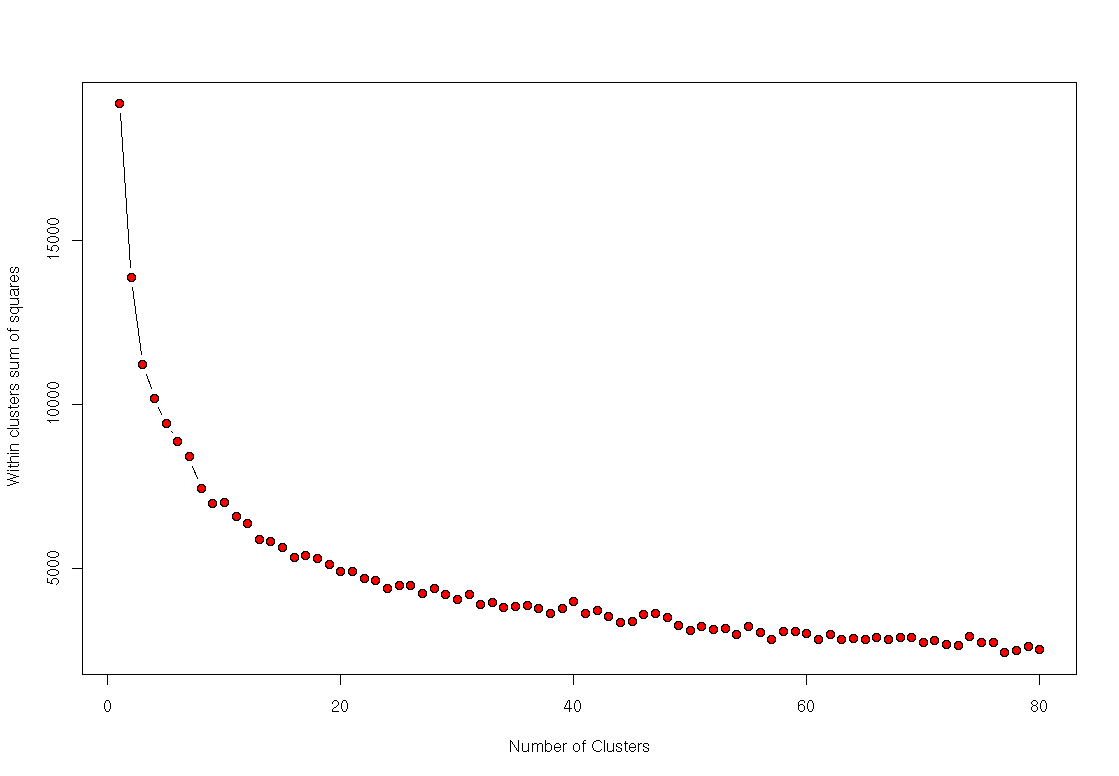
\includegraphics[angle=0, scale=0.35]{hartigan_nuclu_b.png}
\caption{Sum of all within clusters sum of squares against number of 
 clusters for data of all torsion angles in 23S rRNA.}
\label{fig:wss}
\end{figure}

\begin{figure}[H]
\centering
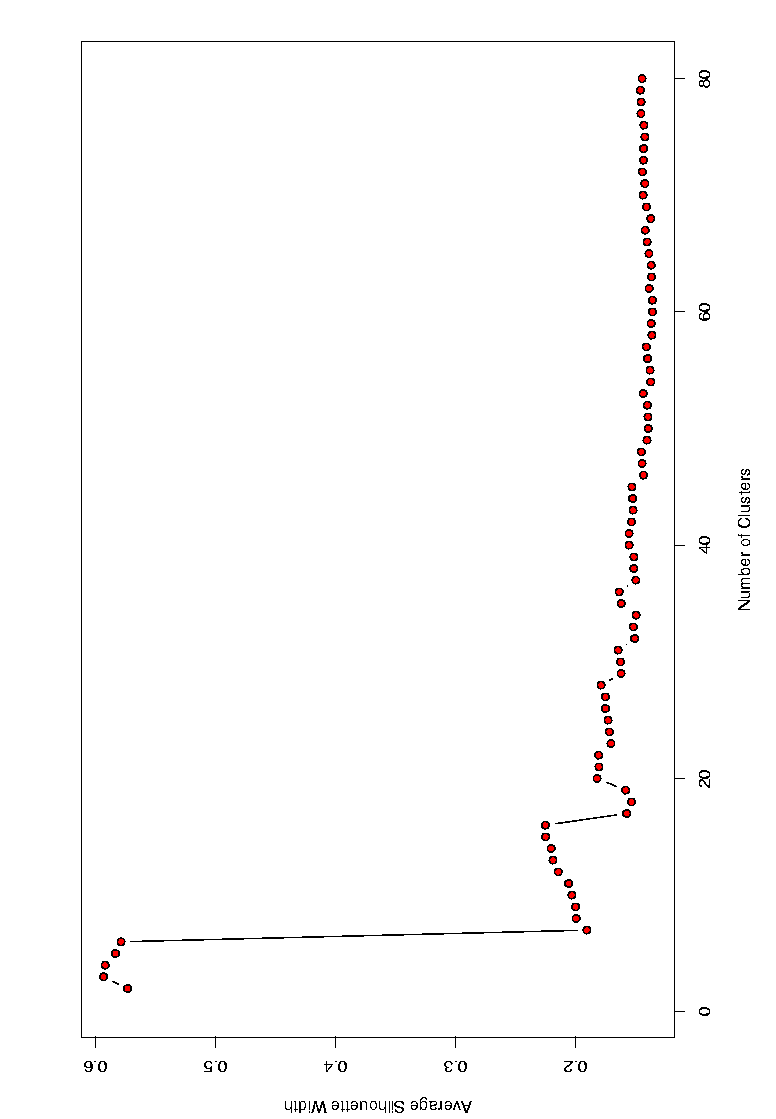
\includegraphics[angle=270, scale=0.48]{pam_asw_2_80_torsions.png}
\caption{Average silhouette width against  number of clusters for data
of  all torsion angles  in 23S  rRNA. The  best clustering  method and
value of $k$ is then defined as the model that maximizes a.s.w.}
\label{fig:asw}
\end{figure}

\begin{figure}
 \centering
 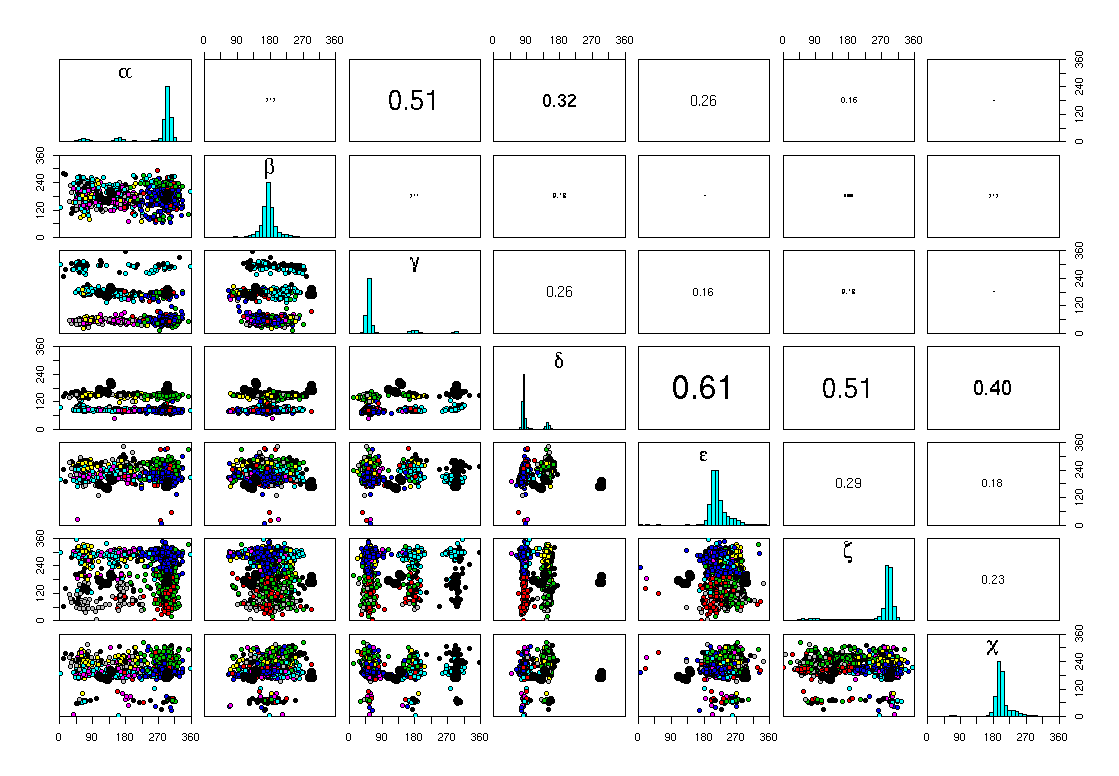
\includegraphics[angle=90, scale=0.50]{hartigan_k8_b.png}
 \caption{K-means clustering of  heptadimensional torsion angle vectors
of  2753  dinucleotide  steps  present  in 23S  rRNA.  The  number  of
partitions  is  \textbf{8}.  The  large  black  dots  represent cluster
centers. The upper diagonal matrix displays the values of the linear
correlation coefficient $r$, and a histogram showing the torsion angle
distribution is rendered in the diagonal.}
 \label{fig:k8}
 \end{figure}
 
\begin{figure}[htbp]
 \centering
 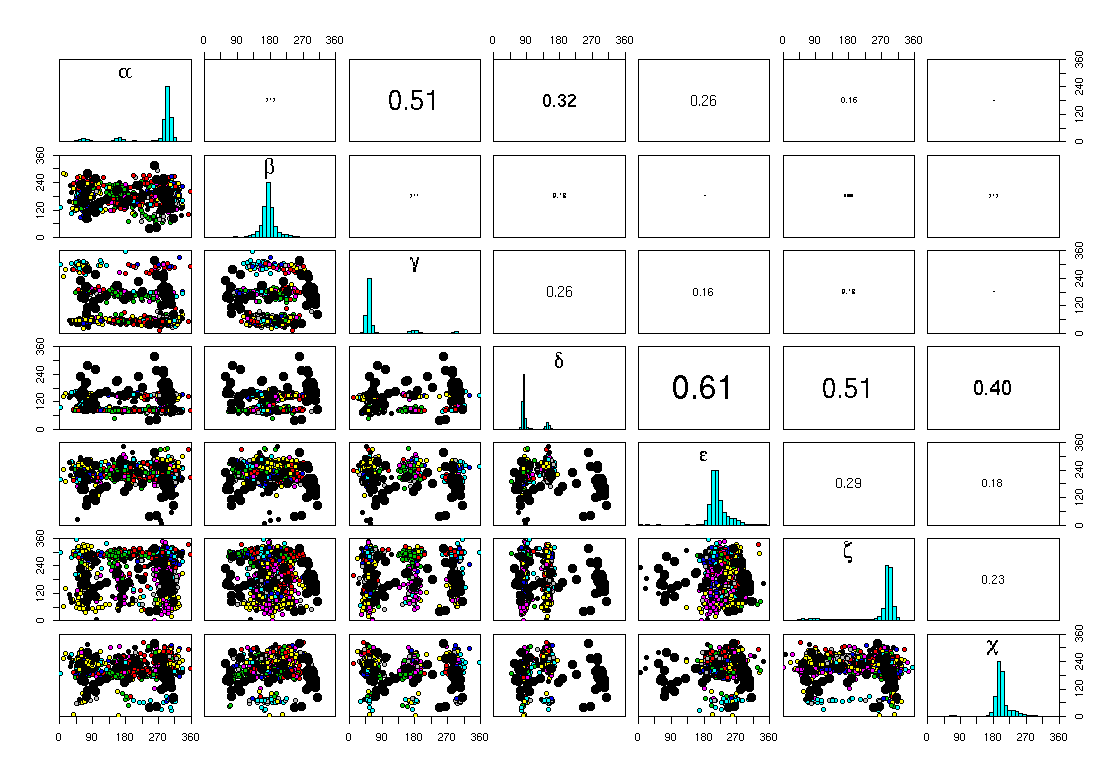
\includegraphics[angle=90, scale=0.50]{hartigan_k60_b.png}
 \caption{K-means clustering of  heptadimensional torsion angle vectors
of  2753  dinucleotide  steps  present  in 23S  rRNA.  The  number  of
partitions  is  \textbf{60}.  The  large  black  dots represent cluster
centers. The upper diagonal matrix displays the values of the linear
correlation coefficient $r$, and a histogram showing the torsion angle
distribution is rendered in the diagonal.}
 \label{fig:k60}
 \end{figure}

\begin{figure}[htbp]
 \centering
 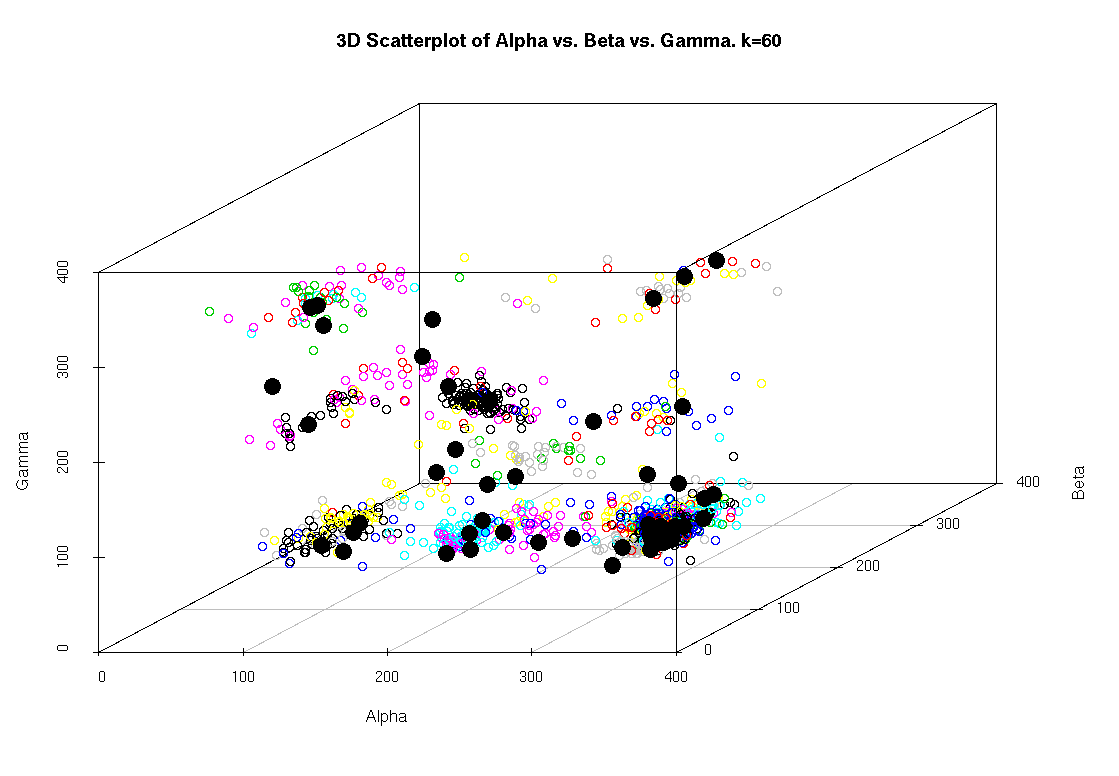
\includegraphics[angle=90, scale=0.50]{hartigan_k60_3D_b.png}
 \caption{K-means  clustering  of  the heptadimensional  torsion  angle
vectors of 2753 dinucleotide steps of  23S rRNA. The axis of the three
dimensional scatterplot  corresponds to the  torsion angles, $\alpha$,
$\beta$,  and $\gamma$.   The  large black  dots  correspond with  the
cluster centers for clustering by using k-means with k=60.}
 \label{fig:3d}
\end{figure}


\subsection{Hierarchical Clustering for Torsion Angles}
Other  authors have  used hierarchical clustering  to analyze the
torsion angles in nucleic acid structure, taking the Fr\"{o}benius
norm and Ward's method as the distance definition
for   four   different    RNA   representations   (see   Reijmers   et
al.  \cite{reijmers2001}) on  a ``small''  database similar to that of
Duarte and Pyle  \cite{duarte1998}. This  databases  do not
include ribosomal RNA's. The other  case where hierarchical clustering
has been used  did not  use torsion  angles, but rather a set  of  15 atoms
belonging  to the  nucleotides sugar  and  backbone. The latter study
used used  the unweighted pair  group method  (UPGMA) to classify  a database  of RNA
loop structures (see Huang et al. \cite{huang2005}).

In our case we  used three distance definitions (Euclidean, Manhattan,
and maximum),  and four  different clustering methodologies,  that is,
single, complete, average  and centroid (see~\ref{appendix_a}. We tried to  make a consensus
analysis of the twelve trees  obtained, but these trees are too large.
The number of trees, that is, twelve, is also too small compared with
the data vectors (2753 step vectors), for  the algorithms to find a  reasonable consensus. 
We were not even able  to find consensus for two  ``near'' clusters, where the
``near''  criteria  was  taken   from  a  tree dissimilarity algorithm
implemented in  \textbf{R}  cluster and   whose   result   can    be   
seen   in Figure~\ref{fig:clusdissim} where the previously mentioned 
``near'' clusters refer to clusters five and nine.  
One  typical  suggestion  in  clustering
analysis is to just use the  single linkage method since this one uses
as  its  grouping  criteria  the minimal  distance  between  clusters,
therefore giving a direct interpretation of the trees as just a direct
minimal  proximity   relation  depending  on  the   metric  being used
(see Appendix~\ref{appendix_a}). \footnote{The  author still has to  do
consensus of single  method trees.}  In  Figure~\ref{fig:hclus} we
see twelve
clustering trees clustering all base-steps in the large subunit of the
ribosome. It's noticeable that trees are more similar  when the linkage
method is the same than when the metric is the same. The main problem 
with the dendrograms in Figure~\ref{fig:hclus} is very similar to that 
of determining the number of partitions in partitional clustering. In
this case we have to determine which is the optimal tree height which 
would determine how many meaningful groups we have, for 
Figure~\ref{fig:hclus} we have selected to draw boxes around a group of 
branches at the height where 36 branches are found. The reason for 
selecting 36 is because this was one of the maxima in Figure~\ref{fig:asw}
and because it´s close to 37, the number of discrete nucleotide conformations
suggested by Hershkovitz et al. \cite{hershkovitz2006}

\begin{figure}[htbp]
\centering
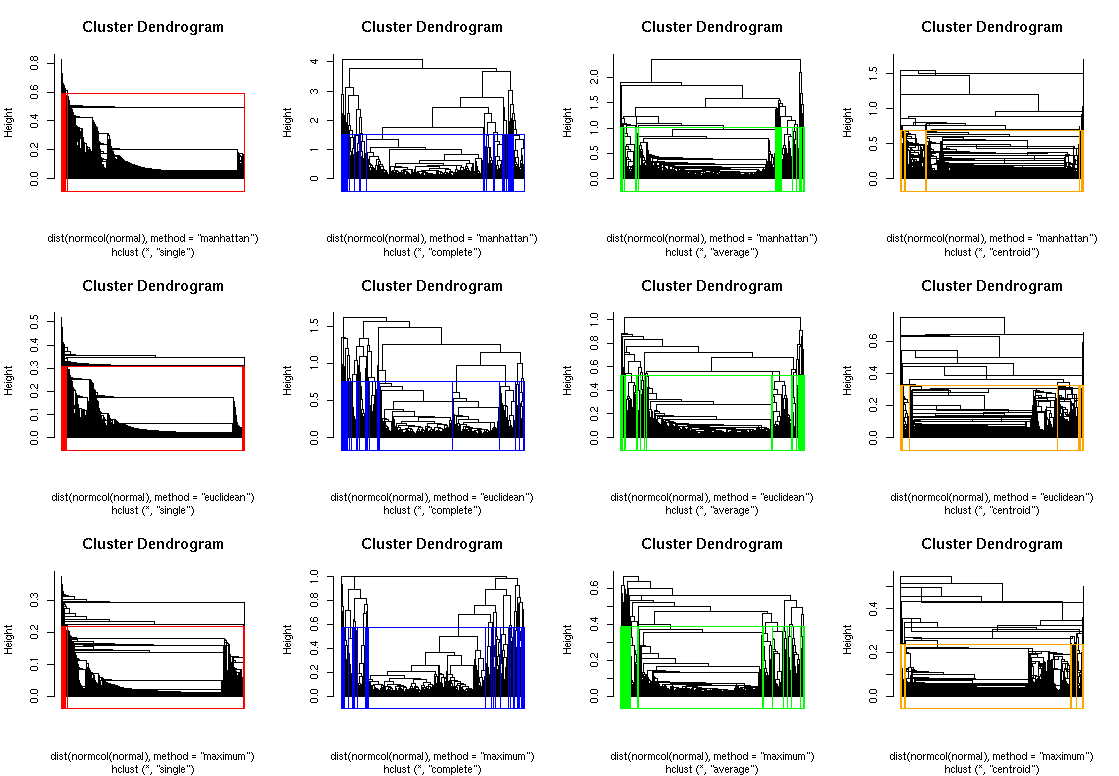
\includegraphics[angle=90, scale=0.55]{treetor_hc.png}
\caption{Hierarchical clustering for the twelve trees
obtained from clustering of torsion angles of the large subunit of 
the ribosome (PDB-ID:1jj2). We have colored a box around branches for the
case where the height of each tree has 36 branches.}
\label{fig:hclus}
\end{figure}

\begin{figure}[htbp]
\centering
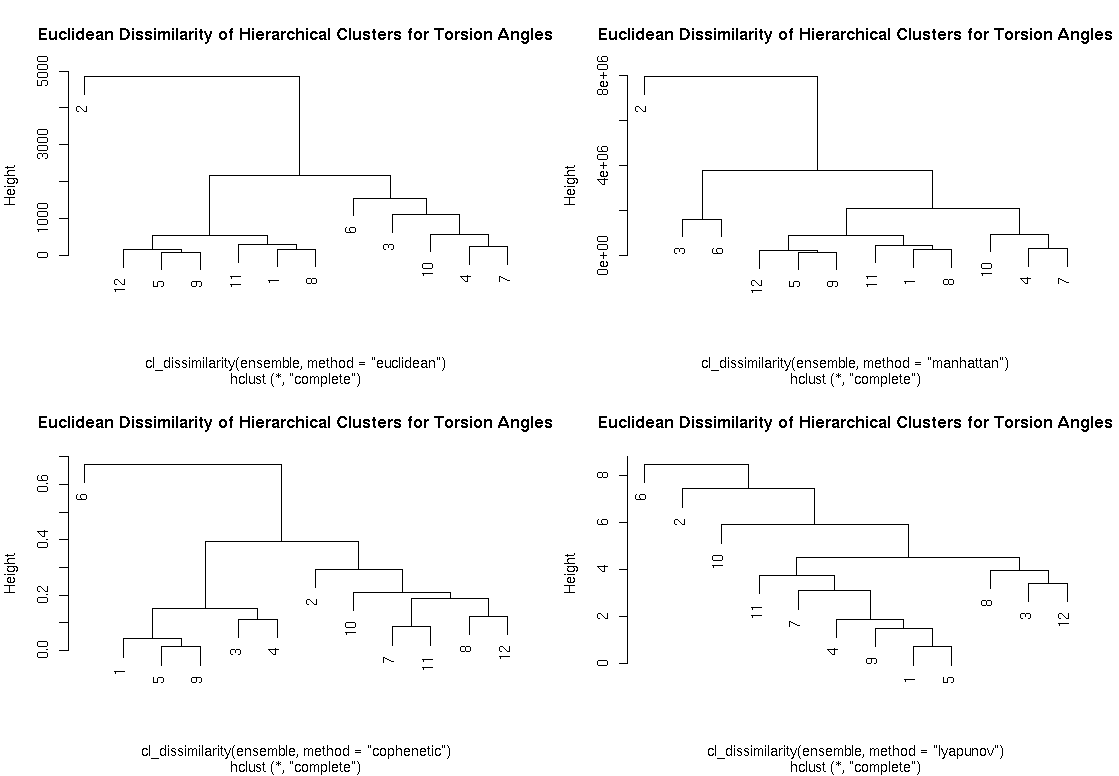
\includegraphics[angle=90, scale=0.60]{clusdissimtor_hc.png}
\caption{Cluster dissimilarities for the 12 combinations of 
metrics and methods used to obtain hierarchical clusterings of the 2753 
heptadimensional torsion  angle vectors of 23S rRNA.}
\label{fig:clusdissim}
\end{figure}


\section{Base-step Parameters}

To our  knowledge there has  been no classification of rigid-body
base-step  parameters for RNA structures deposited at  the
PDB \footnote{The effort of putting together a database for such effort
could be an  interesting project to be considered.}.   It is important
to note here that in  crystal structures, RNA bases are determined more
accurately  than  backbone  torsion  angles,  as  has  been  shown  by
Richardson  and collaborators from  analysis of  van der  Waals steric
clashes.   This can  be seen  more clearly  in Figure~\ref{fig:murray},
reproduced from Richardson's work \cite{murray2003}, where the red
and orange dots  in the backbone atoms region  denote steric clashes and
the green  and yellow  dots in  the base atoms  region denote  very good
agreement with expected van der Waals distances.

\begin{figure}[htbp]
 \centering
 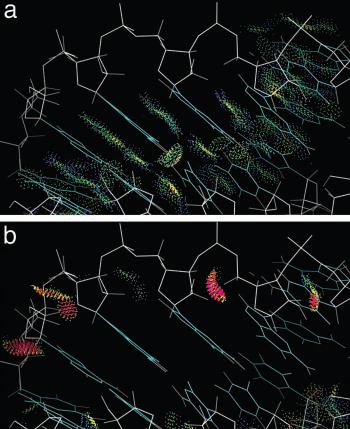
\includegraphics[scale=0.5]{murray2003.png}
 \caption{Figure taken from  Richardson et al. \cite{murray2003} where
 the  blue and  green dots  in  a) mean  very accurate  van der  Waals
 distances, and  in b)  the red and  orange dots mean  steric clashes,
 that is, distances outside the acceptable van der Waals range.}
 \label{fig:murray}
\end{figure}

\subsection{Combining Fourier Averaging Results and Clustering Analysis}
Using the coordinates files of 20 rRNA structures provided by 
Schneider at al.\cite{schneider2004}  we have
used standard clustering analysis (CA) techniques to classify a set of
non-ARNA base-steps  using, rather than the torsion  angles space, the
base-step  parameters space, that  is, three  translational parameters
(Shift$D_x$, Slide$D_y$,  Rise$D_z$), and three  rotational parameters
(Tilt$\tau$,  Roll$\rho$, Twist$\omega$), which  are described  by the
hexaparametric vector $\nu$:

\begin{gather}
 \nu = (D_x, D_y, D_z, \tau, \rho, \omega)
\end{gather}

The     results      illustrated     in     Figures~\ref{fig:eucl_cons}
and~\ref{fig:nonAclus} were  obtained   by   performing  clustering
analysis  and  consensus  clustering  on  20  structures  provided  by
Schneider et  al.  \cite{schneider2004}. These  twenty structures were
obtained  by  Schneider applying  a  Fourier  averaging technique  and
lexicographical  clustering  to  torsion  angles  of  23S  rRNA.   The
methodology  we  used follows  that  used  by  others to  recover  the
periodic table  classification from multidimensional  property vectors
for  elements \cite{restrepo2004,  restrepo2006}. Table~\ref{tab:nonA}
shows the residue  numbers of bases from 23S rRNA  which belong to the
main  categories   of  Figure~\ref{fig:nonAclus}.   To   decide  which
residues of  23S rRNA belonged to  the non-Atype clusters,  a root mean
squared  deviation (RMSD) of  15  or  less  was required  between  step
parameter vectors of  23S rRNA and the mean  parameter vectors for the 
four non-Atype groups identified.

\begin{figure}[htbp]
 \centering
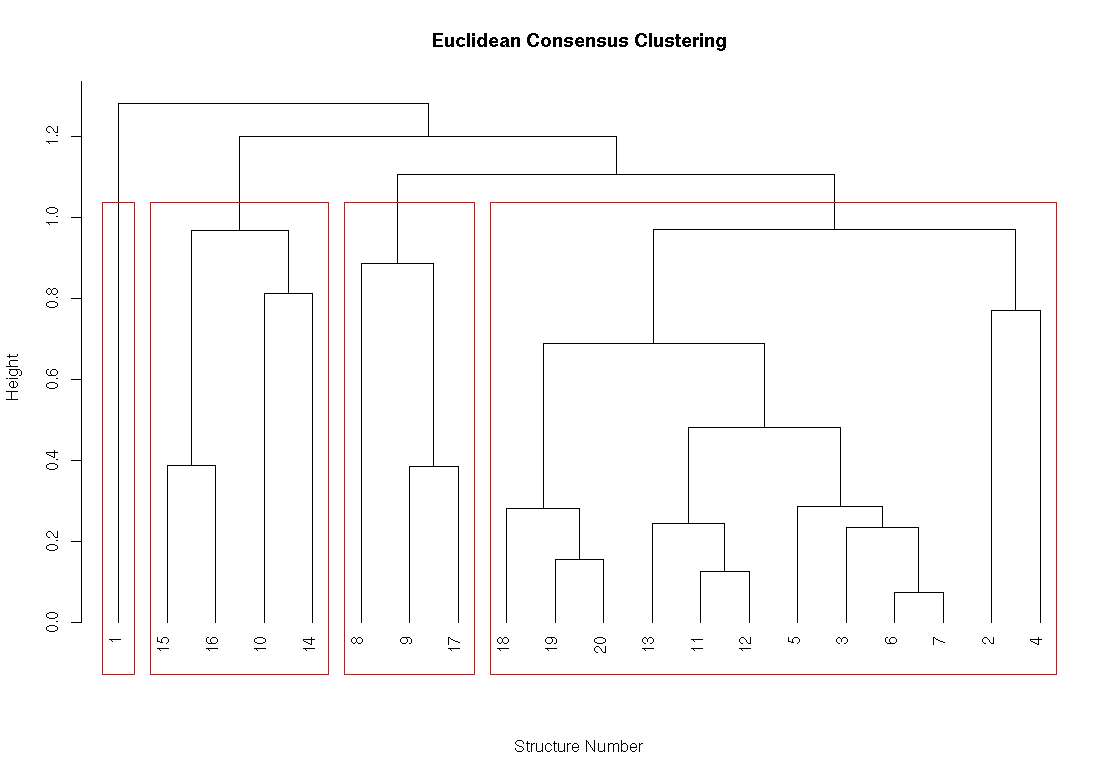
\includegraphics[angle=90, scale=0.6]{eucli_cons_nonA-RNA.png}
\caption{Dendrogram showing the results  of consensus clustering of 20
non-Atype  rRNA  dinucleotides   according  to  their  hexadimensional
base-step parameter vectors.}
 \label{fig:eucl_cons}
\end{figure}

\begin{figure}[htbp]
 \centering
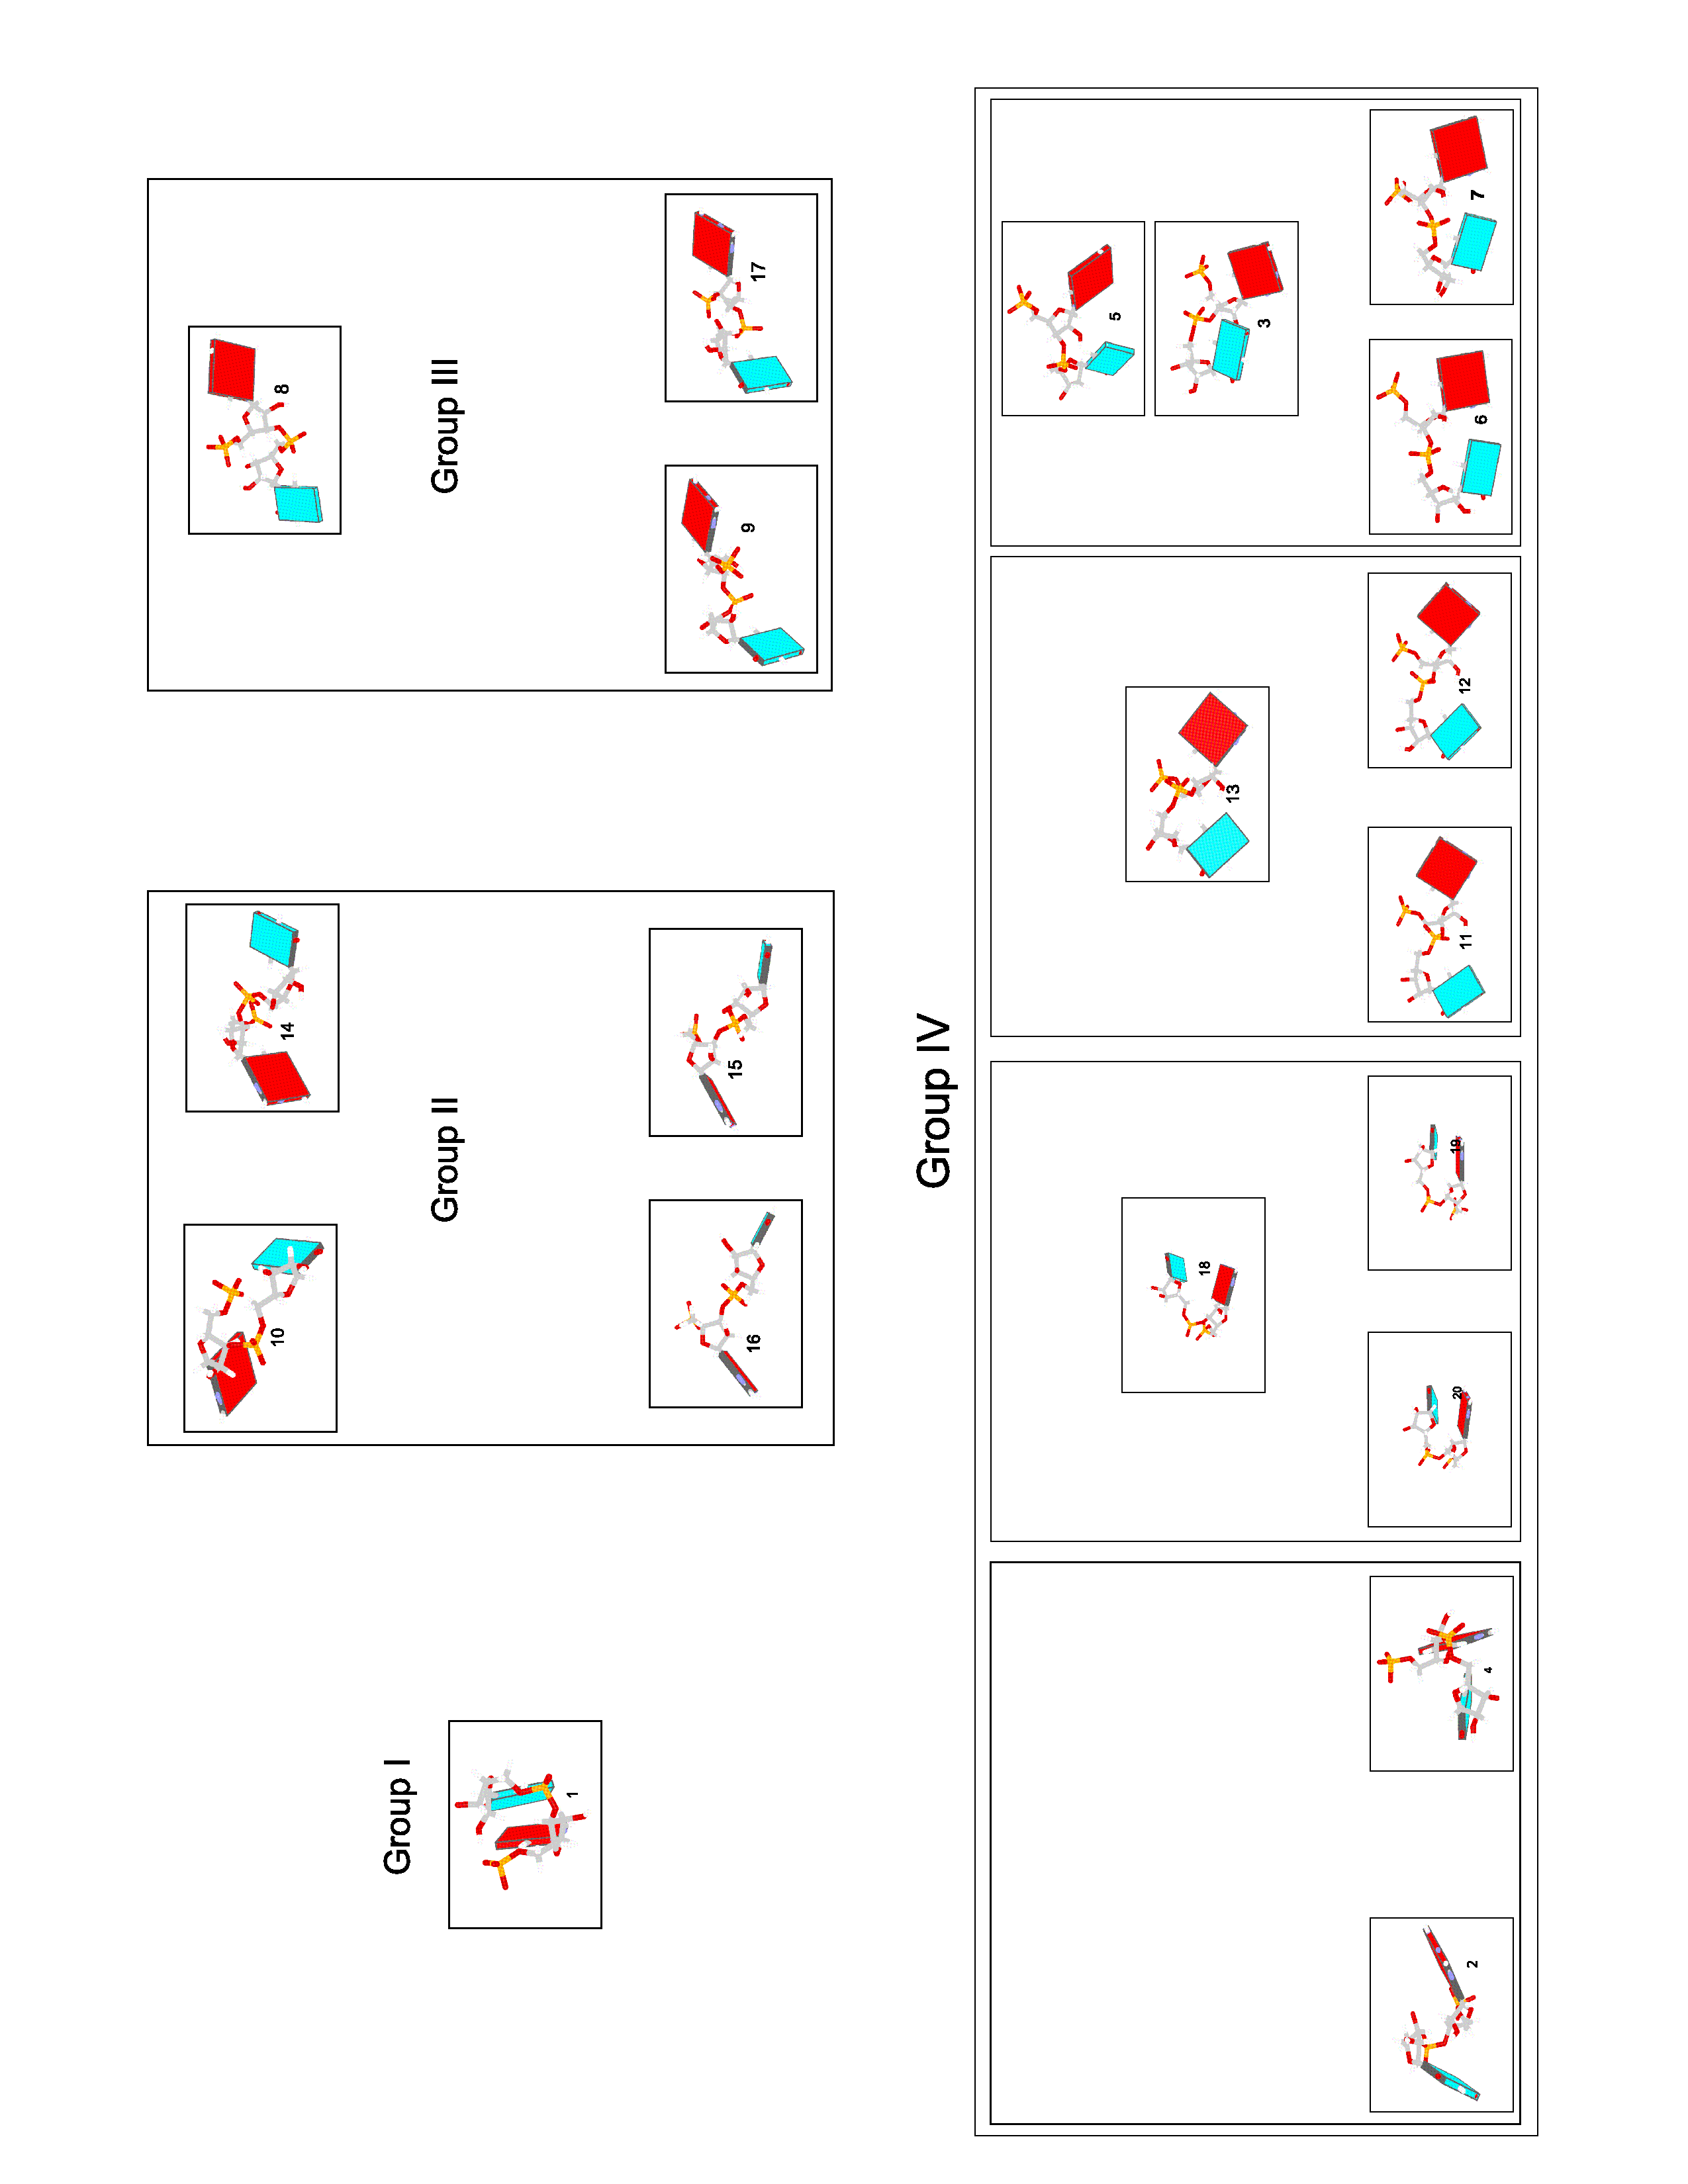
\includegraphics[angle=0, scale=0.8]{Clustered.png}
 \caption{rRNA dinucleotide structures organized by clusters obtained from
consensus clustering of their hexadimensional base-step parameter vectors.}
 \label{fig:nonAclus}
\end{figure}

\begin{table}[htbp]
\begin{center}
{\footnotesize
\begin{tabular}{p{3cm}|p{1,3cm}|c|c|p{3cm}|p{3cm}}
\hline
\bf{Total Number of Nucleotides} & \bf{RMSD Limit} & \bf{Group} & \bf{Base-steps}
& \bf{Base-step Residue Number} & \bf{Overlaps} \\ \hline
2754 & $ < 15$ & I & 3 & 892, 2006, 2390 &  \\ \hline
 &  & II & 5 & 459, 1279, 1653, 1919, 2302 &  \\ \hline
 &  & III & 1 & 2109 &  \\ \hline
 &  & IV & 35 & 79, 112, 128, 190, 213, 269, 358, 434, 488, 564, 706,
 720, 775, 867, 966, 1292, 1503, 1543, 1614, 1766, 1874, 1908, 1971, 
 2017, 2257, 2427, 2516, 2540, 2755, 2782, 2810, 2826, 2874, 2882, 2913 &  \\ \hline
 &  & IVa & 1 & 882 &  \\ \hline
 &  & IVb & 807 &  &  \\ \hline
 &  & IVc & 9 & 306, 789, 854, 880, 1107, 1192, 1493, 1818, 2005 &  \\ \hline
 &  & IVd & 35 & 175, 213, 246, 264, 304, 358, 464, 518, 531, 534,
 588, 795, 938, 1214, 1231, 1316, 1340, 1370, 1605, 1745, 1766, 
 1971, 1976, 2010, 2017, 2291, 2320, 2428, 2469, 2481, 2516, 2532, 
 2755, 2826, 2882 & Only IVd with IV (213, 358, 1766, 1971, 2017, 
 2516, 2755, 2826, 2882) \\ \hline
\end{tabular}
}
\caption{Residue numbers for base-steps  with RMSD values less than 15
between  the  reference base-step  vectors  from  the  four groups  of
non-A-type  RNA dinucleotide conformations  and all  base-step vectors
found  in  the 23S  strand  of  \textit{Haloarcula marismortui}  large
ribosomal subunit.}
\label{tab:nonA}
\end{center}
\end{table}


\subsection{Partitional Clustering for Rigid Body Parameters}

The same type of analysis that has been carried out for torsion angles
can  also  be  carried  out   for  rigid  body  parameters,  that  is,
partitional  clustering, and  hierarchical  clustering, are used  as 
standard statistical  analysis methods  to analyze  our set  of  2753 
base-step parameter vectors.  For the  partitional clustering case, 
again, there is no known number of clusters in which the data must
group, therefore we've  calculated the  within clusters  sum  of
squares and also  the
average silhouette widths, for a particular selection of the number of
partitions of the data for $k=[2-80]$.  From figure~\ref{fig:wssSteps}
we can't conclude  much. We see that the value  of the within clusters
sum  of squares  becomes constant  around  $k=47$ and  there´s also  a
change of  curvature around  $k=13$.  For the  case where  the average
silhoutte width has been computed, that is, figure~\ref{fig:aswSteps},
we see that  the maximum is for $k=2$, and  there are some interesting
maxima at  $k=9,12$.  Now that  we have a  clue as to which  number of
partitions the data  optimally has we have plotted  the k-means results
for $k=13$ and $k=47$ in Figures  bla and bla, and the PAM results for
$k=2, 9, 12$ in Figure bla.


We have  also prefiltered  the data according  to the 16  possible RNA
base steps, that is,  AA, AG, GA, GG, UU, UC, CU,  CC, UA, UG, CA, CG,
AU, AC,  GU, and  GC.  Tables showing  how many  representatives steps
there are  belonging to  non-helical, helical, and  watson-crick sets,
will be later included and discussed here.

\begin{figure}[htbp]
\centering
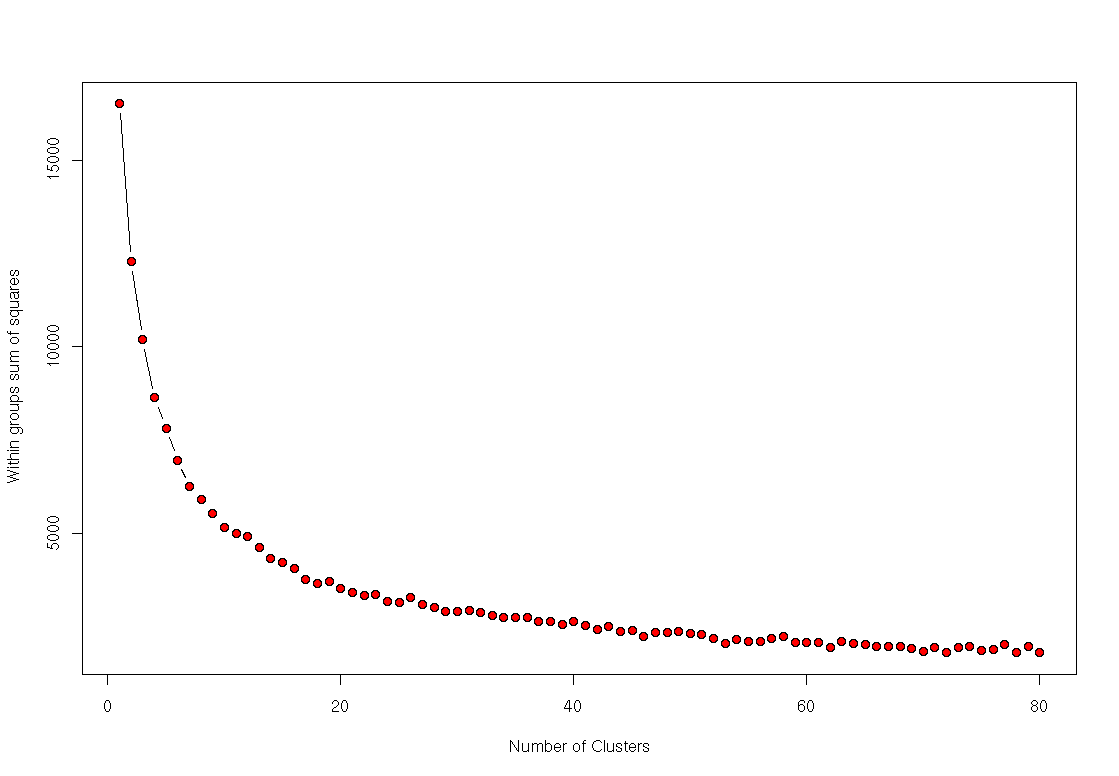
\includegraphics[angle=0, scale=0.40]{hartigan_nuclu_steps_b.png}
\caption{Sum of all within clusters sum of squares against number of clusters.}
\label{fig:wssSteps}
\end{figure}

\begin{figure}[htbp]
 \centering
 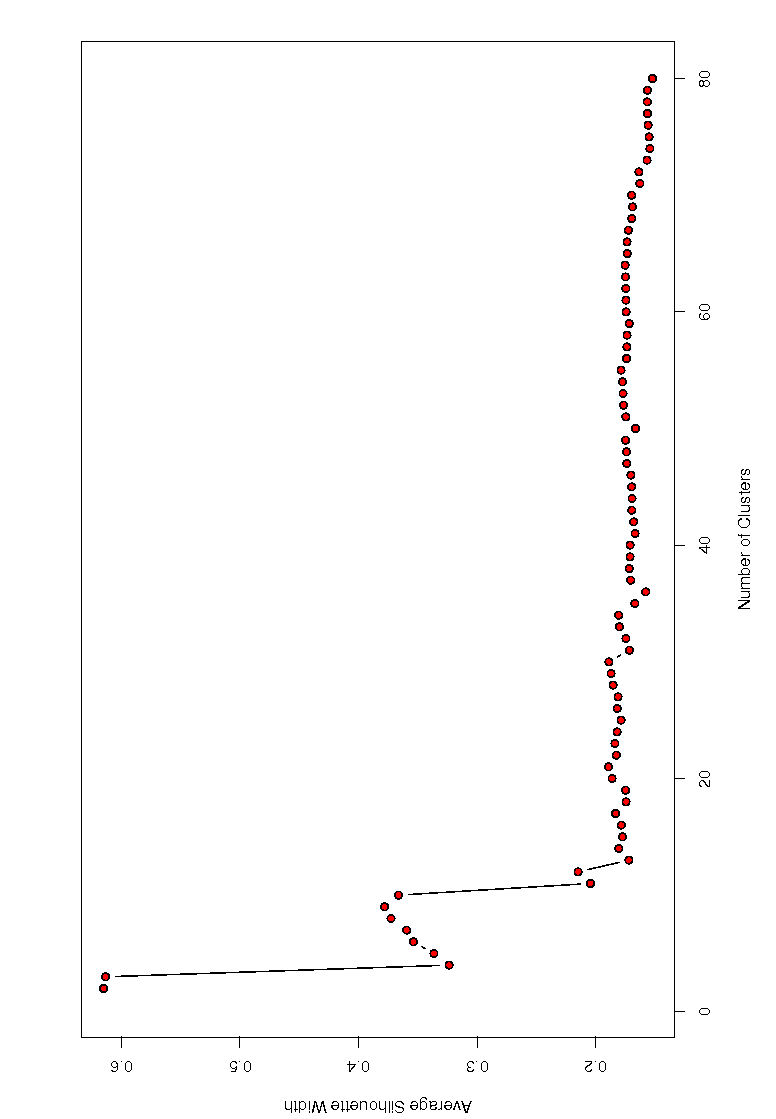
\includegraphics[angle=270, scale=0.50]{pam_asw_2_80_steps.png}
 \caption{Average silhouette width against number of clusters.}
 \label{fig:aswSteps}
\end{figure}



\subsection{Hierarchical Clustering for Rigid Body Parameters}

Also as has been carried out for torsion angles, hierarchical clustering has
also been performed on rigid body parameters, the results are yet to be
included here. A cluster dissimilarity tree can be seen in
Figure~\ref{fig:clusdis} for the 12 trees resulting from the four clustering
methods and three distance definitions used to cluster the base step data.

\begin{figure}[htbp]
\centering
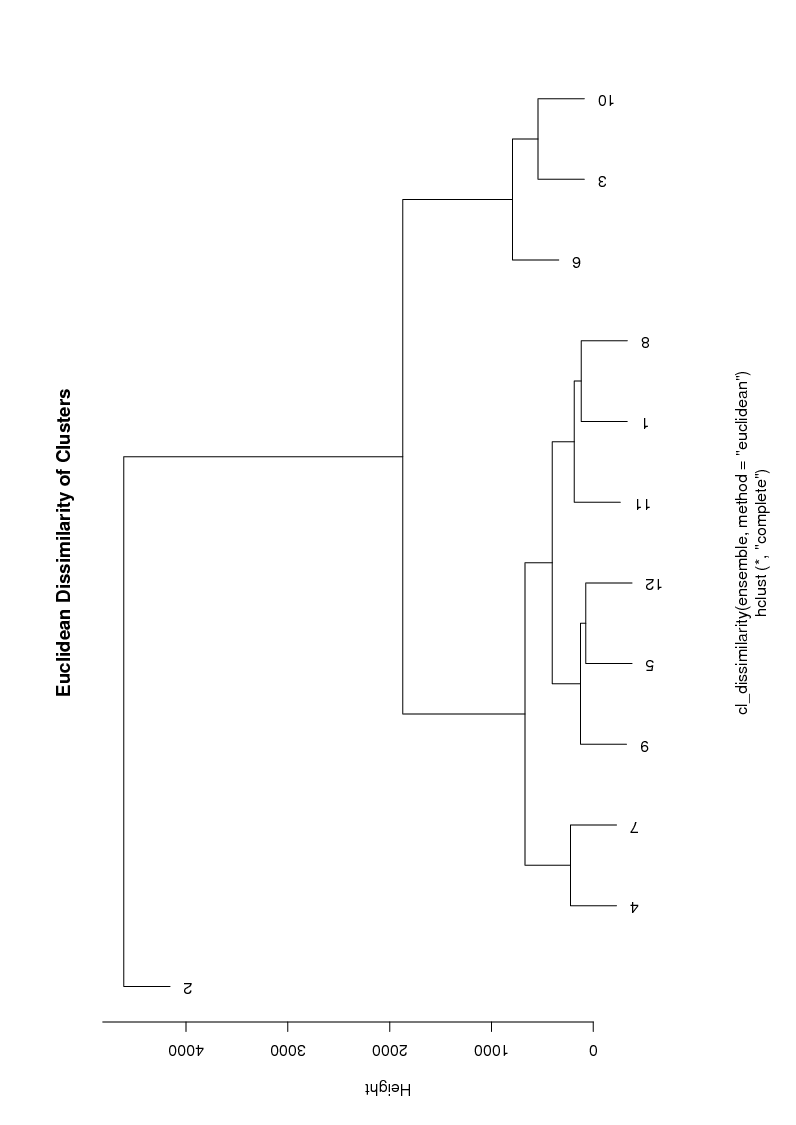
\includegraphics[scale=0.60]{clussdissim.png}
\caption{Cluster dissimilarities for the twelve hierarchical trees
  obtained from clustering of the six-dimensional base-step parameters
obtained from the large subunit of the ribosome (PDB-ID:1jj2)}
\label{fig:clusdis}
\end{figure}


\section{RNA Conformations}
There are two main RNA conformations, A-RNA ,and A'RNA, and maybe even a
third unconfirmed one A"RNA \cite{saenger1984}.
Their values for their standard torsion angles and step parameters can be seen
in Tables~\ref{tab:tor_conf} and ~\ref{tab:step_conf} 

\begin{table}[htbp]
\begin{center}
{\small
\begin{tabular}{c|c|c|c|c|c|c|c|c}
\hline
\bf{Structure Name} & $\alpha$ & $\beta$ & $\gamma$ & $\delta$ & $\epsilon$
& $\zeta$ & $\chi$ & \bf{Reference} \\ \hline
A-RNA & -68.9 & 179.5 & 54.5 & 82.2 & -153.9 & -70.8 & -161.1 & Arnott \\ \hline
A'-RNA & -70.0 & 176.6 & 60.8 & 76.7 & -153.4 & -69.4 & -163.4 & Arnott \\ \hline
AII-RNA & -65.0 & 175.1 & 52.9 & 81.1 & -166.0 & -68.0 & -157.0 & Schneider \\ \hline
\end{tabular}
}
\caption{Base step torsion angles for the different known RNA conformations.}
\label{tab:tor_conf}
\end{center}
\end{table}

\begin{table}[htbp]
\begin{center}
{\small
\begin{tabular}{p{2cm}|c|c|c|c|c|c|c}
\hline
\bf{Structure Name} & Shift ($D_x$) & Slide ($D_y$) & Rise ($D_z$) & Tilt
($\tau$) & Roll ($\rho$) & Twist ($\Omega$) & \bf{Reference} \\ \hline
A-DNA & 0.36 & -1.39 & 3.29 & 2.46 & 12.50 & 30.19 & \\ \hline
B-DNA & 0.44 & 0.47 & 3.33 & 4.63 & 1.77 & 35.67 & \\ \hline
A-RNA & -0.08 & -1.48 & 3.30 & -0.43 & 8.64 & 31.57 & Arnott \\ \hline
A'-RNA & 0.05 & -1.88 & 3.39 & -0.12 & 5.43 & 29.52 & Arnott \\ \hline
AII-RNA & 1.01 & -2.52 & 3.33 & 2.94 & 9.75 & 25.12 & Schneider \\ \hline
\end{tabular}
}
\caption{Base step parameters for the different known RNA
  conformations. Notice that the base step parameters are for single
  bases rather than base-pairs.}
\label{tab:step_conf}
\end{center}
\end{table}




\begin{figure}[htbp]
\centering
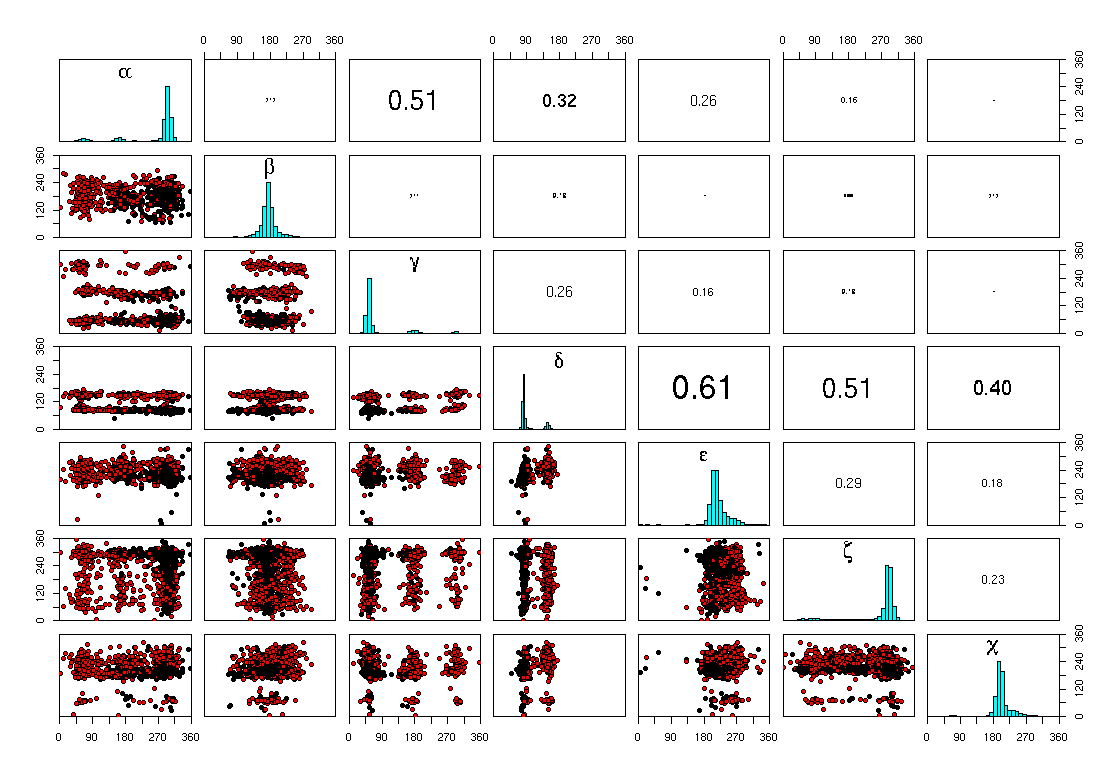
\includegraphics[angle=90, scale=0.50]{hartigan_tor_b.png}
\caption{
K-means of torsion  angle vectors of 2753 dinucleotide steps
present in  23S rRNA using the  \textit{Hartigan-Wong} algorithm.  The
number  of  partitions  is  \textbf{2}.   The  upper  diagonal  matrix
displays the values  of the linear correlation coefficient  $r$, and a
histogram showing  the torsion angle distribution is rendered  in the
diagonal.}
\label{fig:hartigan}
\end{figure}

\begin{figure}[htbp]
\centering
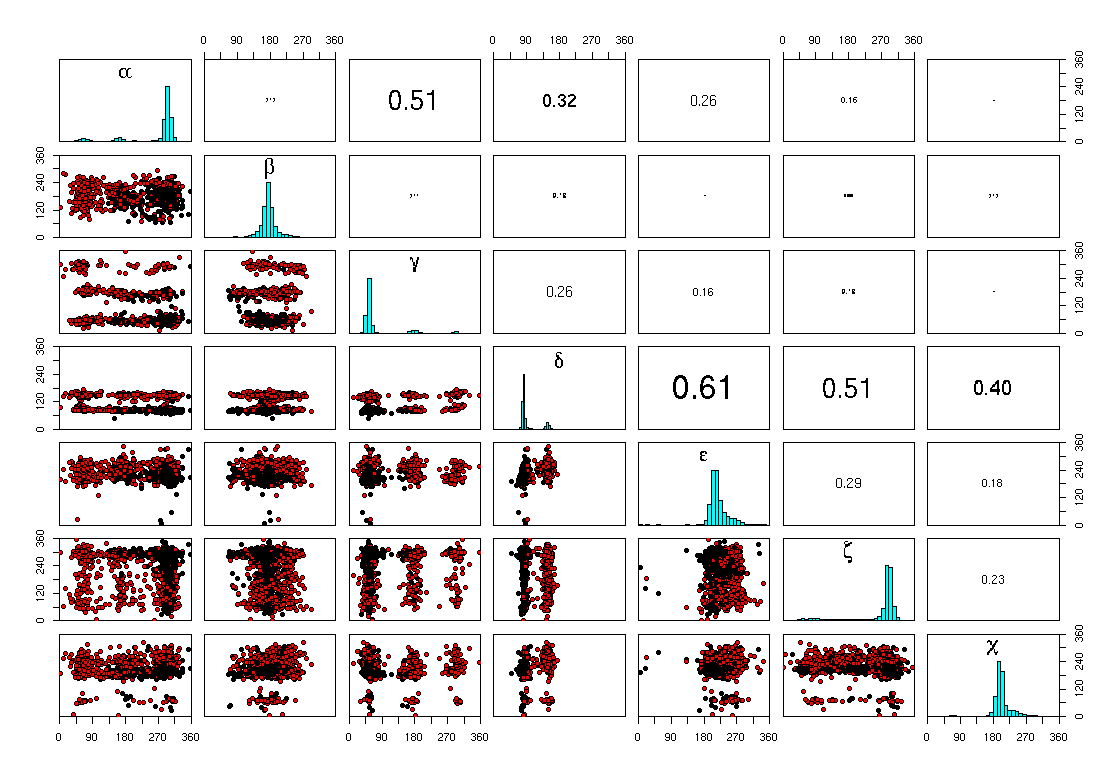
\includegraphics[angle=90, scale=0.50]{lloyd_tor_b.png}
\caption{
K-means of torsion  angle vectors of 2753 dinucleotide steps
present in  23S rRNA using the  \textit{Lloyd} algorithm.  The
number  of  partitions  is  \textbf{2}.   The  upper  diagonal  matrix
displays the values  of the linear correlation coefficient  $r$, and a
histogram showing  the torsion angle  distribution is rendered  in the
diagonal.}
\end{figure}

\begin{figure}[htbp]
\centering
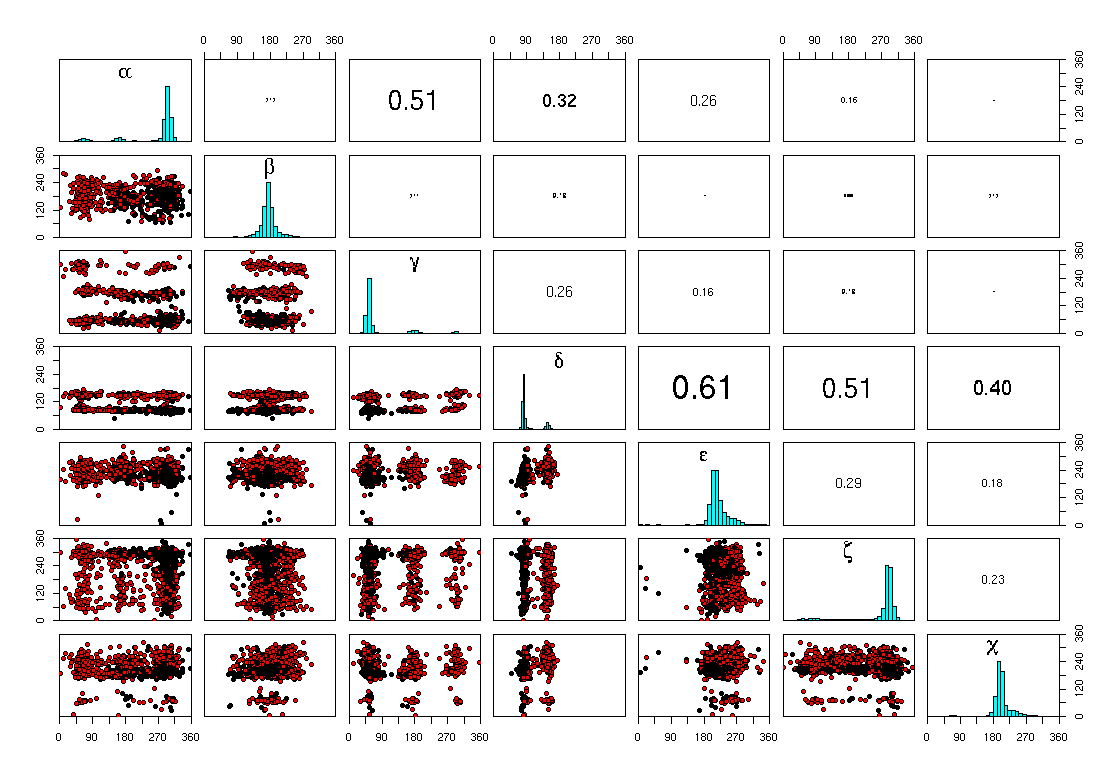
\includegraphics[angle=90, scale=0.50]{forgy_tor_b.png}
\caption{
K-means of torsion  angle vectors of 2753 dinucleotide steps
present in  23S rRNA using the  \textit{Forgy} algorithm.  The
number  of  partitions  is  \textbf{2}.   The  upper  diagonal  matrix
displays the values  of the linear correlation coefficient  $r$, and a
histogram showing  the torsion angle  distribution is rendered  in the
diagonal.}
\end{figure}

\begin{figure}[htbp]
\centering
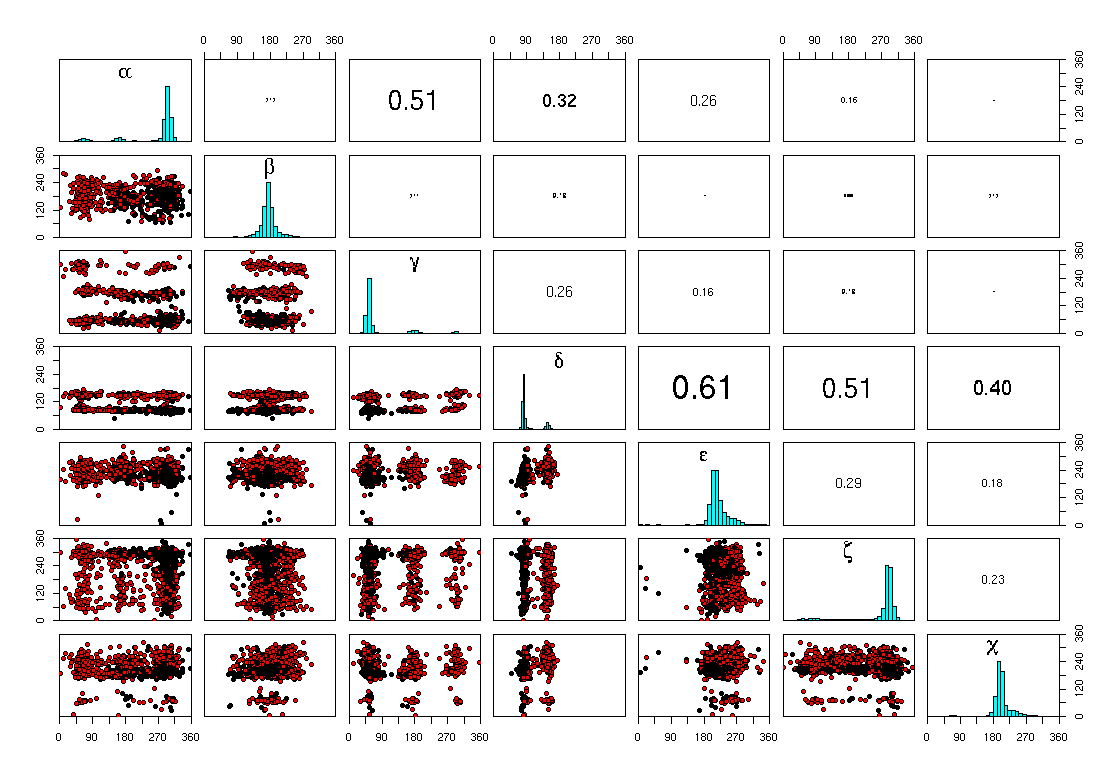
\includegraphics[angle=90, scale=0.50]{macqueen_tor_b.png}
\caption{
K-means of torsion  angle vectors of 2753 dinucleotide steps
present in  23S rRNA using the  \textit{McQueen} algorithm.  The
number  of  partitions  is  \textbf{2}.   The  upper  diagonal  matrix
displays the values  of the linear correlation coefficient  $r$, and a
histogram showing  the torsion angle  distribution is rendered  in the
diagonal.}
\label{fig:macqueen}
\end{figure}


%\bibliography{../BibTex/thesis}
\bibliography{biblio}
%\bibliographystyle{unsrt} or {nar}
\printindex

    \chapter{Sequence Analysis of Ribosomal Step Parameters}
%\bibliographystyle{nar}
\label{sequence} 

For the 2007 IMA Meeting, ``RNA in Biology, Bioengineering and
Nanotechnology'', that took place from October 29 to November 2, 2007 in
Minneapolis, Minnesota, we sorted the base-steps of rRNA
according to 16 possible sequence base-steps, that is, Purine-Purine
(RR: AA, AG, GA, GG), Pyrimidine-Pyrimidine (YY: UU, UC, CU, CC),
Pyrimidine-Purine (YR: UA, UG, CA, CG), and Purine-Pyrimidine (RY: AU,
AC, GU, GC).
In Table~\ref{tab:distribution} we show how these 16 base-steps
distribute in the complete rRNA structure (All), in the helical regions of
rRNA found by the 3DNA software (Helical), and in base-steps whose
first member is part of a Watson-Crick (WC) base-pair.

\begin{table}[htbp]
\begin{center}
{\small
%\begin{tabular}{|c|p{1cm}|c|c|c|}
\begin{tabular}{|c|c|c|c|c|}
\hline
\multicolumn{2}{|c|}{Ribosome  50S}& All & Helical & Watson-Crick \\ \hline
RR & AA & 202 & 102 & 12  \\ \hline
   & AG & 232 & 164 & 60  \\ \hline
   & GA & 250 & 177 & 64  \\ \hline
   & GG & 249 & 238 & 160 \\ \hline
YY & UU & 75  & 54  & 20  \\ \hline
   & UC & 147 & 107 & 66  \\ \hline
   & CU & 142 & 123 & 78  \\ \hline
   & CC & 200 & 186 & 137 \\ \hline
YR & UA & 124 & 90  & 24  \\ \hline
   & UG & 176 & 143 & 62  \\ \hline
   & CA & 163 & 96  & 60  \\ \hline
   & CG & 226 & 192 & 126 \\ \hline
RY & AU & 116 & 79  & 37  \\ \hline
   & AC & 189 & 127 & 60  \\ \hline
   & GU & 188 & 141 & 90  \\ \hline
   & GC & 196 & 181 & 94  \\ \hline
\end{tabular}
}
\caption{Distribution of base-step types in rRNA (PDB-ID:1jj2)}
\label{tab:distribution}
\end{center}
\end{table}


In Tables~\ref{tab:average1} and ~\ref{tab:average2} we show the average values and
the standard deviation for the base-step parameters for the 16
dinucleotide steps.


\begin{table}[htbp]
\begin{center}
{\small
%\begin{tabular}{|c|p{1cm}|c|c|c|}
\begin{tabular}{|c|c|c|c|c|c|c|c|c|c|}
\hline
 & \multicolumn{3}{|c|}{Shift} 
 & \multicolumn{3}{|c|}{Slide} 
 & \multicolumn{3}{|c|}{Rise} \\ \hline
 & All & Helical & W-C & All & Helical & W-C &
   All & Helical & W-C \\ \hline
AA(mean) &-0.409 & 0.826 & -0.133 & -0.559 & -0.418 & -1.999 & 2.604 & 2.226 & 2.919 \\ \hline
AA(sd)  & 6.780 & 3.535 & 0.611 & 2.708 & 2.389 & 0.980 & 5.101 & 2.487 & 0.934 \\ \hline     
AG(mean) &0.639 & 2.245 & 0.614 & -1.157 & -1.161 & -1.719 & 2.982 & 3.110 & 3.151 \\ \hline  
AG(sd)  & 6.494 & 3.160 & 1.199 & 2.457 & 1.747 & 1.152 & 3.913 & 1.458 & 0.429 \\ \hline     
GA(mean) &-3.286 & -2.142 & 0.578 & -1.776 & -1.549 & -1.851 & 2.867 & 2.645 & 3.086 \\ \hline
GA(sd)  & 6.193 & 4.100 & 0.855 & 2.413 & 2.078 & 0.768 & 3.575 & 2.784 & 0.672 \\ \hline     
GG(mean) &0.316 & 0.545 & 0.763 & -1.705 & -1.839 & -2.064 & 2.936 & 3.072 & 3.196 \\ \hline  
GG(sd)  & 3.595 & 1.633 & 1.171 & 1.527 & 1.120 & 0.665 & 2.278 & 0.935 & 0.425 \\ \hline     
UU(mean) &-0.989 & -0.095 & 0.761 & -1.073 & -1.087 & -1.623 & 2.762 & 2.480 & 3.174 \\ \hline
UU(sd)  & 6.087 & 2.306 & 1.022 & 1.914 & 1.921 & 0.677 & 4.192 & 2.314 & 0.268 \\ \hline     
UC(mean) &-0.010 & 0.421 & 0.138 & -1.460 & -1.298 & -1.519 & 3.379 & 3.047 & 3.322 \\ \hline 
UC(sd)  & 6.121 & 2.071 & 1.124 & 1.693 & 0.944 & 0.867 & 3.678 & 1.332 & 0.345 \\ \hline     
CU(mean) &0.289 & 0.581 & 0.596 & -1.435 & -1.432 & -1.539 & 3.191 & 3.278 & 3.385 \\ \hline  
CU(sd)  & 4.303 & 1.708 & 0.857 & 1.077 & 1.080 & 0.696 & 2.546 & 0.942 & 0.584 \\ \hline     
CC(mean) &0.472 & 0.244 & 0.165 & -1.604 & -1.546 & -1.619 & 3.635 & 3.404 & 3.437 \\ \hline  
CC(sd)  & 3.352 & 1.414 & 0.938 & 1.066 & 0.781 & 0.500 & 1.857 & 1.139 & 0.491 \\ \hline     
UA(mean) &-2.232 & -0.773 & 0.402 & -1.282 & -1.445 & -1.466 & 3.048 & 2.330 & 2.938 \\ \hline
UA(sd)  & 7.180 & 3.037 & 0.474 & 2.278 & 1.736 & 0.769 & 4.314 & 2.851 & 0.885 \\ \hline     
UG(mean) &-0.712 & 0.413 & 0.396 & -1.278 & -1.095 & -1.660 & 2.545 & 2.800 & 3.220 \\ \hline 
UG(sd)  & 7.044 & 2.445 & 1.115 & 2.750 & 1.547 & 0.473 & 3.828 & 1.879 & 0.458 \\ \hline     
CA(mean) &-0.566 & 0.271 & 0.175 & -1.159 & -1.173 & -1.254 & 3.109 & 2.877 & 3.119 \\ \hline 
CA(sd)  & 6.379 & 1.807 & 1.440 & 2.629 & 1.633 & 1.211 & 4.472 & 1.471 & 1.050 \\ \hline     
CG(mean) &0.932 & 0.873 & 0.807 & -1.207 & -1.333 & -1.638 & 3.459 & 2.878 & 3.331 \\ \hline  
CG(sd)  & 5.131 & 1.910 & 1.589 & 1.910 & 1.035 & 0.638 & 3.181 & 1.398 & 0.419 \\ \hline     
AU(mean) &-1.586 & 1.181 & 0.848 & -0.050 & -0.805 & -1.288 & 1.935 & 2.518 & 3.088 \\ \hline 
AU(sd)  & 10.773 & 2.062 & 1.267 & 11.914 & 1.628 & 0.399 & 5.399 & 1.934 & 0.238 \\ \hline   
AC(mean) &0.247 & 1.535 & 0.823 & -1.200 & -1.161 & -1.406 & 2.856 & 2.950 & 3.191 \\ \hline  
AC(sd)  & 5.753 & 2.532 & 0.802 & 1.761 & 1.074 & 0.600 & 3.724 & 1.631 & 0.556 \\ \hline     
GU(mean) &-0.899 & 0.580 & 0.838 & -1.630 & -1.496 & -1.473 & 2.887 & 2.937 & 3.004 \\ \hline 
GU(sd)  & 5.842 & 2.115 & 1.232 & 1.843 & 1.101 & 0.596 & 3.196 & 0.898 & 0.471 \\ \hline     
GC(mean) &-0.450 & 0.663 & 0.584 & -1.520 & -1.351 & -1.539 & 2.633 & 2.730 & 3.047 \\ \hline 
GC(sd)  & 5.351 & 1.430 & 1.240 & 1.422 & 1.266 & 1.209 & 2.720 & 1.317 & 0.764 \\ \hline       
\end{tabular}
}
\caption{Average base-step parameters Shift($D_x$), Slide($D_y$), and
Rise($D_z$), and their standard deviations for the 
16 possible specific dinucleotide base-steps in rRNA (PDB-ID:1jj2)}
\label{tab:average1}
\end{center}
\end{table}



\begin{table}[htbp]
\begin{center}
{\small
%\begin{tabular}{|c|p{1cm}|c|c|c|}
\begin{tabular}{|c|c|c|c|c|c|c|c|c|c|}
\hline
 & \multicolumn{3}{|c|}{Tilt} 
 & \multicolumn{3}{|c|}{Roll} 
 & \multicolumn{3}{|c|}{Twist} \\ \hline
 & All & Helical & W-C & All & Helical & W-C &
   All & Helical & W-C \\ \hline
AA(mean) &1.752 & -3.965 & -8.317 & 3.130 & 2.794 & 1.794 & 20.757 & 28.123 & 39.992 \\ \hline   
AA(sd)  & 52.388 & 46.911 & 43.597 & 43.872 & 48.766 & 12.441 & 61.833 & 69.499 & 44.488 \\ \hline
AG(mean) &1.660 & -0.290 & 4.970 & -2.915 & 6.432 & 6.909 & 29.437 & 44.960 & 30.366 \\ \hline   
AG(sd)  & 40.762 & 33.407 & 12.249 & 54.999 & 44.517 & 17.874 & 60.077 & 49.794 & 14.675 \\ \hline
GA(mean) &1.524 & 7.486 & 2.774 & 5.657 & 3.350 & 1.891 & 0.303 & 23.609 & 32.426 \\ \hline      
GA(sd)  & 40.488 & 48.392 & 8.416 & 47.487 & 38.171 & 18.947 & 62.473 & 52.173 & 10.706 \\ \hline
GG(mean) &4.767 & -0.406 & 2.018 & 2.980 & 0.242 & 4.702 & 27.322 & 35.409 & 34.969 \\ \hline    
GG(sd)  & 26.889 & 29.679 & 13.127 & 25.556 & 30.270 & 10.133 & 35.549 & 25.956 & 14.067 \\ \hline
UU(mean) &4.590 & 7.830 & 4.119 & 14.585 & 2.299 & 7.251 & 17.974 & 26.520 & 32.371 \\ \hline    
UU(sd)  & 45.485 & 42.449 & 6.192 & 38.878 & 37.830 & 6.406 & 59.460 & 50.909 & 6.669 \\ \hline  
UC(mean) &-3.746 & 3.885 & 2.690 & 5.659 & 10.155 & 7.935 & 24.156 & 34.421 & 35.726 \\ \hline   
UC(sd)  & 45.258 & 19.279 & 6.744 & 38.300 & 27.183 & 6.568 & 61.100 & 33.273 & 17.096 \\ \hline 
CU(mean) &1.586 & -0.455 & 0.619 & 15.989 & 11.728 & 7.085 & 31.730 & 35.311 & 31.520 \\ \hline  
CU(sd)  & 31.071 & 15.965 & 9.664 & 28.484 & 34.158 & 20.490 & 39.764 & 32.381 & 8.130 \\ \hline 
CC(mean) &-2.865 & -0.014 & -0.817 & 13.487 & 12.353 & 12.499 & 33.396 & 35.132 & 31.231 \\ \hline
CC(sd)  & 20.623 & 19.864 & 9.442 & 21.393 & 21.634 & 23.199 & 29.108 & 22.634 & 15.752 \\ \hline
UA(mean) &-5.082 & 17.366 & 5.997 & 15.921 & 13.854 & 5.854 & 14.453 & 23.904 & 31.072 \\ \hline 
UA(sd)  & 48.747 & 60.210 & 35.883 & 44.432 & 50.073 & 33.762 & 69.347 & 70.086 & 21.478 \\ \hline
UG(mean) &2.816 & 11.150 & 2.876 & 11.702 & 11.719 & 11.405 & 16.030 & 35.716 & 31.355 \\ \hline 
UG(sd)  & 44.717 & 34.923 & 4.588 & 35.585 & 35.347 & 7.323 & 69.936 & 41.080 & 7.587 \\ \hline  
CA(mean) &-5.424 & 1.918 & 4.473 & 18.541 & 14.010 & 12.131 & 27.438 & 33.751 & 25.556 \\ \hline 
CA(sd)  & 46.535 & 32.314 & 33.935 & 49.656 & 51.725 & 36.917 & 64.201 & 44.243 & 37.512 \\ \hline
CG(mean) &-3.526 & 6.437 & -1.149 & 8.030 & 7.857 & 10.392 & 31.739 & 31.399 & 33.078 \\ \hline  
CG(sd)  & 35.351 & 54.584 & 16.207 & 29.225 & 15.785 & 6.968 & 48.690 & 43.902 & 18.347 \\ \hline
AU(mean) &4.660 & -3.373 & 6.439 & 12.288 & 11.167 & 7.512 & 18.943 & 22.843 & 34.141 \\ \hline  
AU(sd)  & 50.513 & 56.862 & 5.414 & 35.199 & 56.726 & 5.386 & 71.378 & 53.225 & 9.904 \\ \hline  
AC(mean) &4.070 & 5.696 & 6.374 & 5.919 & 4.142 & 1.707 & 27.191 & 42.259 & 33.983 \\ \hline     
AC(sd)  & 40.408 & 26.459 & 5.253 & 34.583 & 31.050 & 16.098 & 56.979 & 39.818 & 6.101 \\ \hline 
GU(mean) &5.035 & 3.387 & 7.095 & 7.111 & 6.286 & 7.078 & 21.209 & 40.686 & 38.729 \\ \hline     
GU(sd)  & 35.221 & 26.999 & 6.432 & 33.337 & 29.488 & 18.139 & 50.758 & 30.847 & 15.570 \\ \hline
GC(mean) &5.477 & 6.392 & 7.383 & 9.002 & -0.112 & -0.117 & 22.118 & 33.511 & 31.661 \\ \hline   
GC(sd)  & 30.625 & 43.730 & 9.615 & 34.766 & 28.612 & 24.074 & 52.357 & 36.615 & 24.642 \\ \hline
\end{tabular}
}
\caption{Average base-step parameters Tilt($\tau$), Roll($\rho$), and Twist($\omega$), and their standard deviations for the 
16 possible specific dinucleotide base-steps in rRNA (PDB-ID:1jj2)}
\label{tab:average2}
\end{center}
\end{table}

Once we have classified the base-step parameters for dinucleotide
steps according to sequence we can also plot them automatically in a
pairs plot. Such automatic plots, which have not been scaled according
to a specific scale, are quite useful to identify uncommon
base-steps. \textbf{Whether such uncommon base-step parameter values are due
to bad cristallographic results, or to intrinsic structural
peculiarities of such base-steps seems to be a question worthy of being addressed.}
In Figures~\ref{fig:stepsAA} to~\ref{fig:stepsGC}

%%%%%%%%%%%%%%%%%%%%%%%%%%%%%%%%%%%%%%%%%%%%%%%%%
%THE FOLLOWING ARE THE SCATTERPLOTS FOR ALL STEPS
%%%%%%%%%%%%%%%%%%%%%%%%%%%%%%%%%%%%%%%%%%%%%%%%

\begin{figure}[H]
\centering
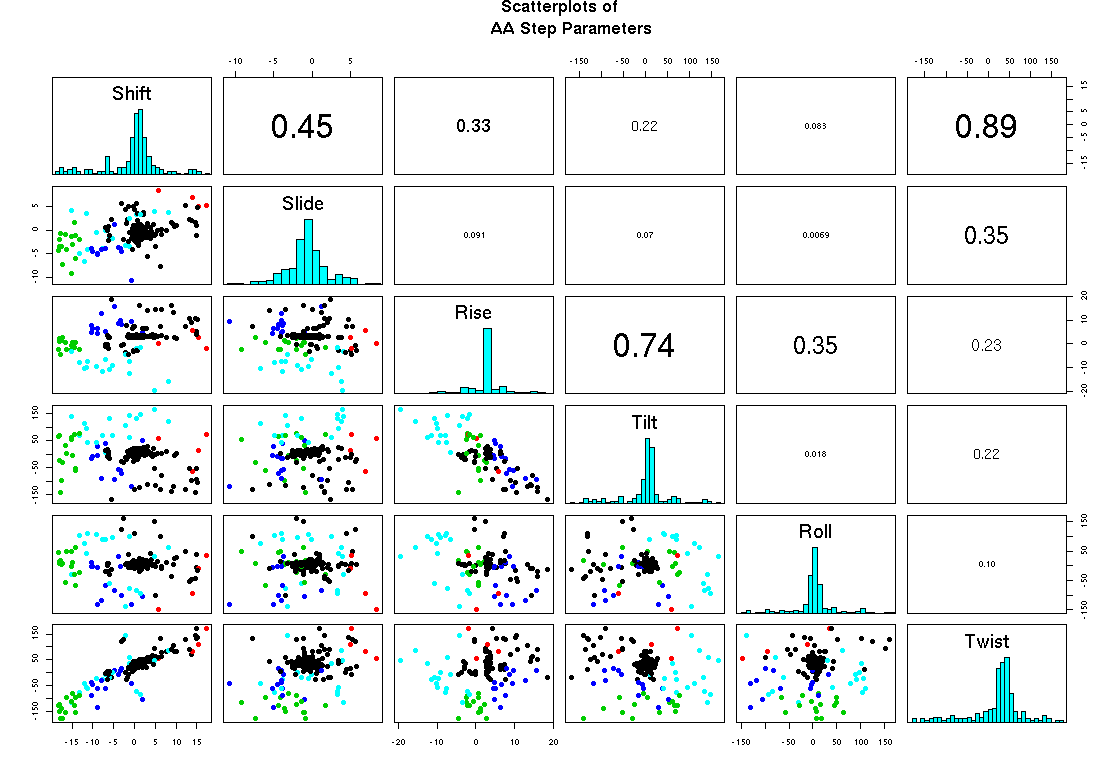
\includegraphics[angle=90, scale=0.6]{All/AA.png}
\caption{Scatterplots for step-parameters of \textbf{All} AA dinucleotide steps
in 50S rRNA.}
\label{fig:stepsAA}
\end{figure}

\begin{figure}[H]
\centering
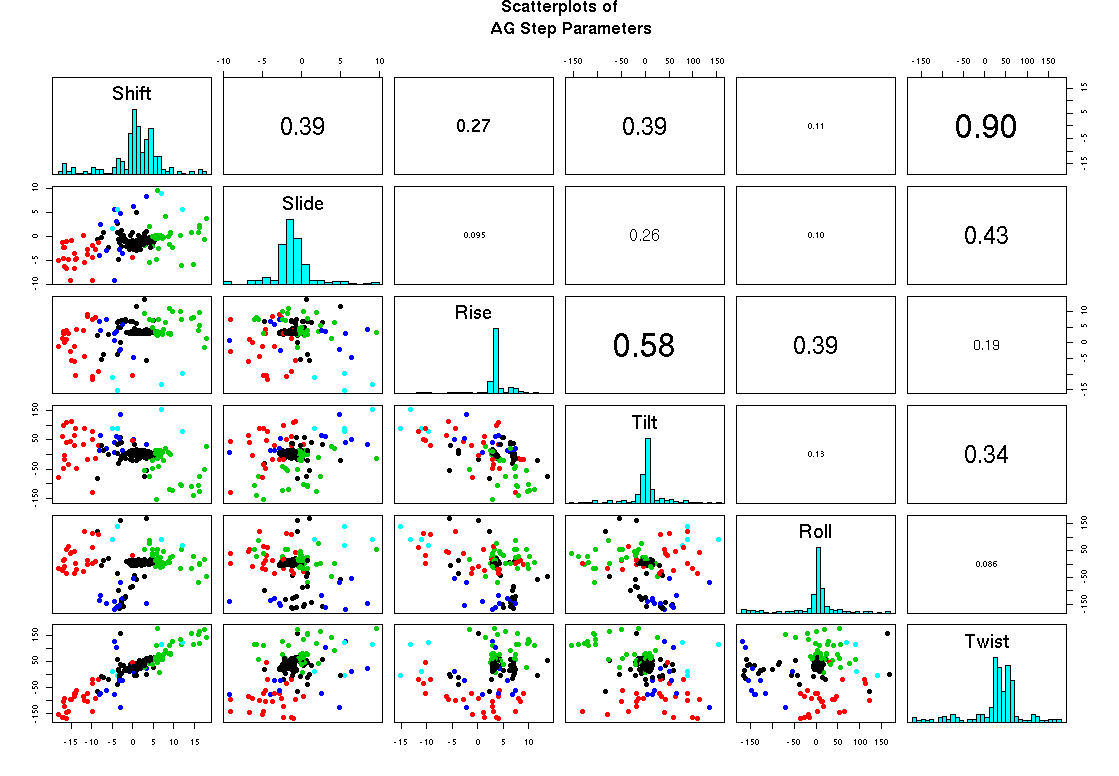
\includegraphics[angle=90, scale=0.6]{All/AG.png}
\caption{Scatterplots for step-parameters of \textbf{All} AG dinucleotide steps
in 50S rRNA.}
\label{fig:stepsAG}
\end{figure}

\begin{figure}[H]
\centering
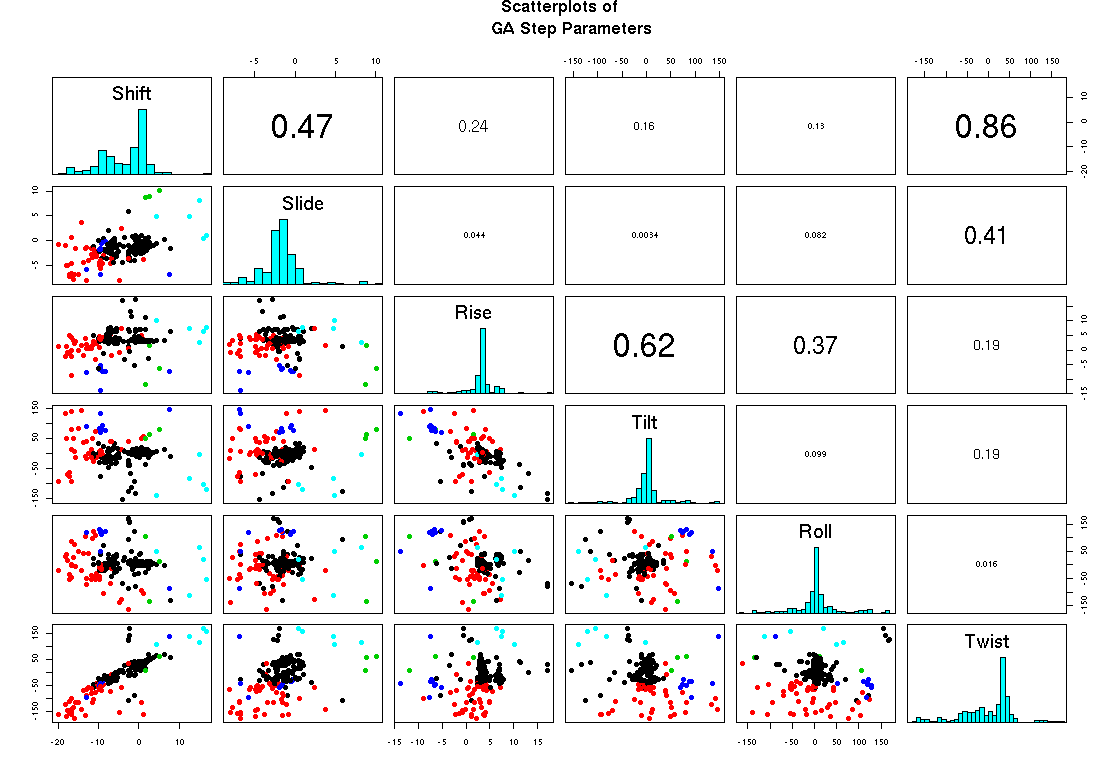
\includegraphics[angle=90, scale=0.6]{All/GA.png}
\caption{Scatterplots for step-parameters of \textbf{All} GA dinucleotide steps
in 50S rRNA.}
\label{fig:stepsGA}
\end{figure}

\begin{figure}[H]
\centering
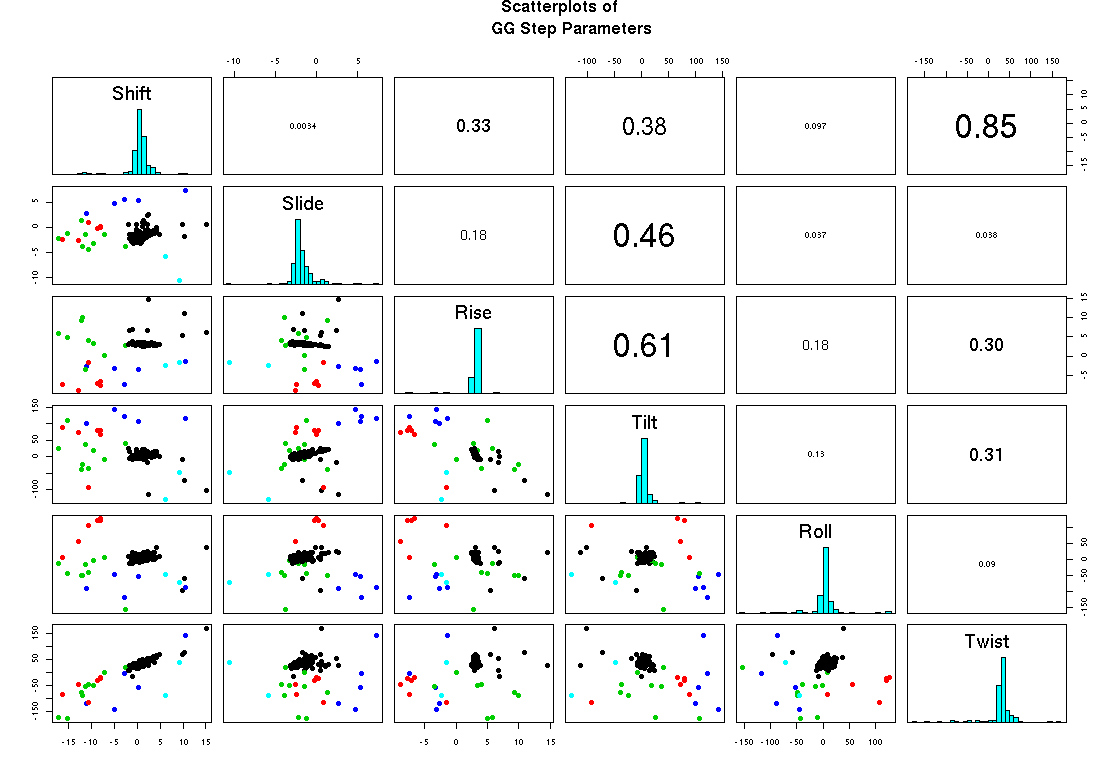
\includegraphics[angle=90, scale=0.6]{All/GG.png}
\caption{Scatterplots for step-parameters of \textbf{All} GG dinucleotide steps
in 50S rRNA.}
\label{fig:stepsGG}
\end{figure}

\begin{figure}[H]
\centering
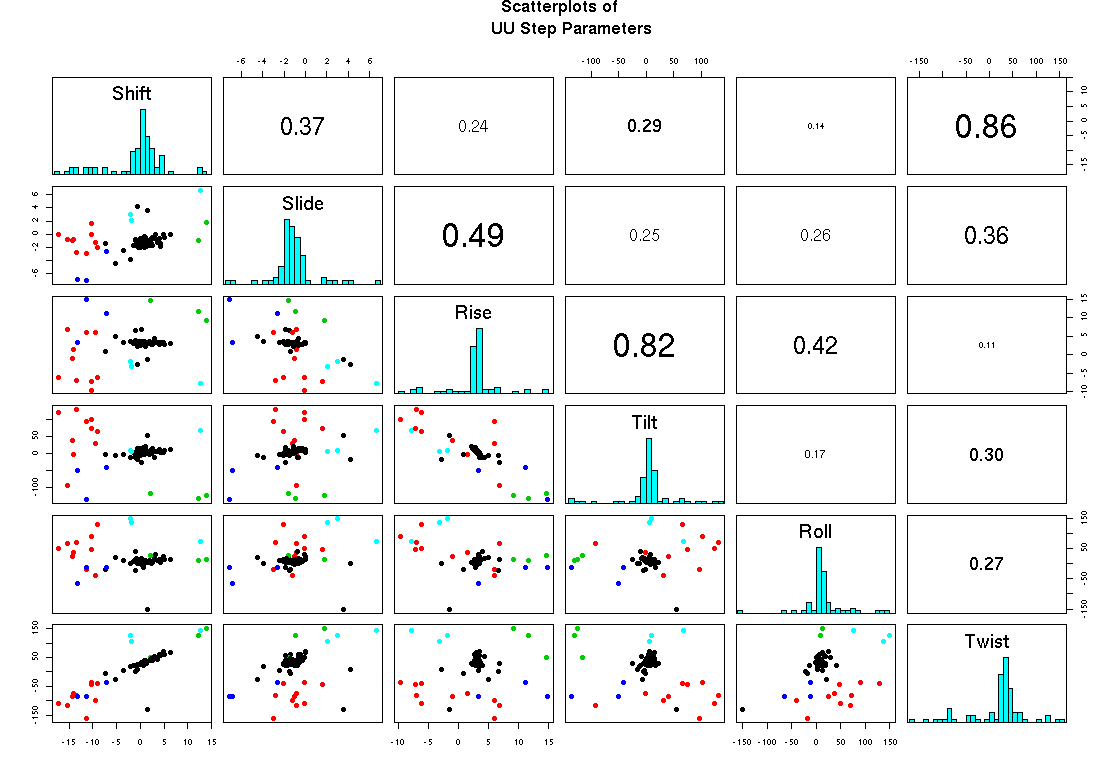
\includegraphics[angle=90, scale=0.6]{All/UU.png}
\caption{Scatterplots for step-parameters of \textbf{All} UU dinucleotide steps
in 50S rRNA.}
\label{fig:stepsUU}
\end{figure}

\begin{figure}[H]
\centering
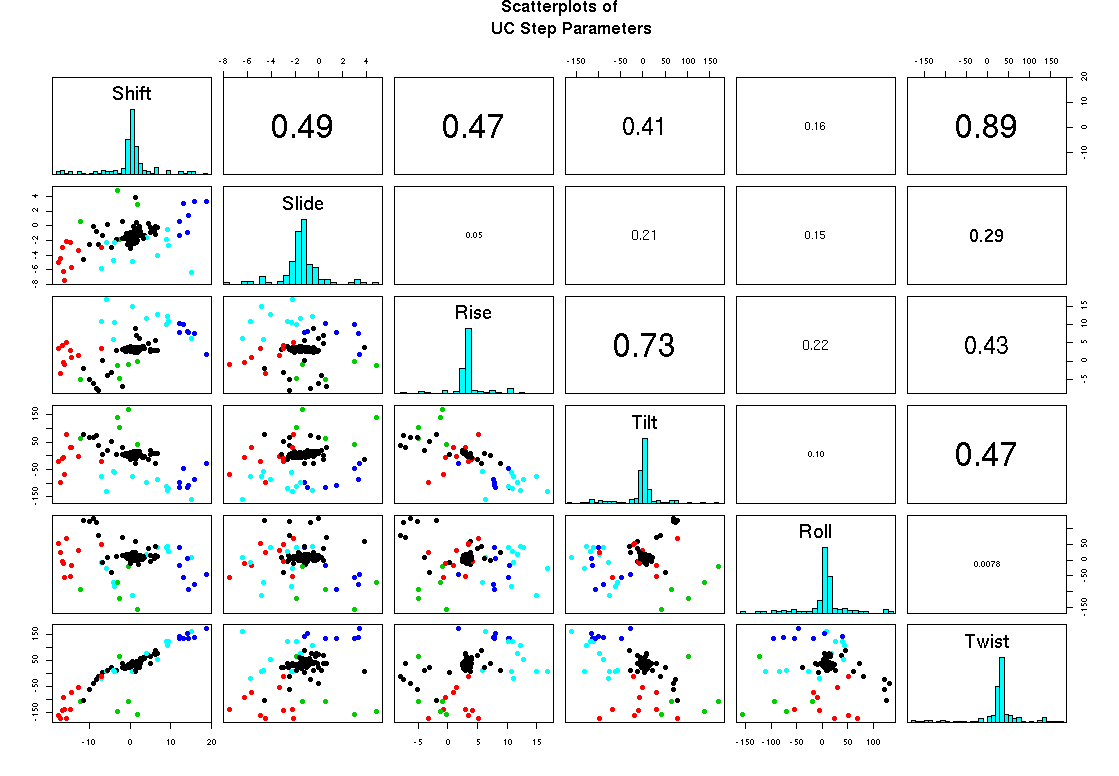
\includegraphics[angle=90, scale=0.6]{All/UC.png}
\caption{Scatterplots for step-parameters of \textbf{All} UC dinucleotide steps
in 50S rRNA.}
\label{fig:stepsUC}
\end{figure}

\begin{figure}[H]
\centering
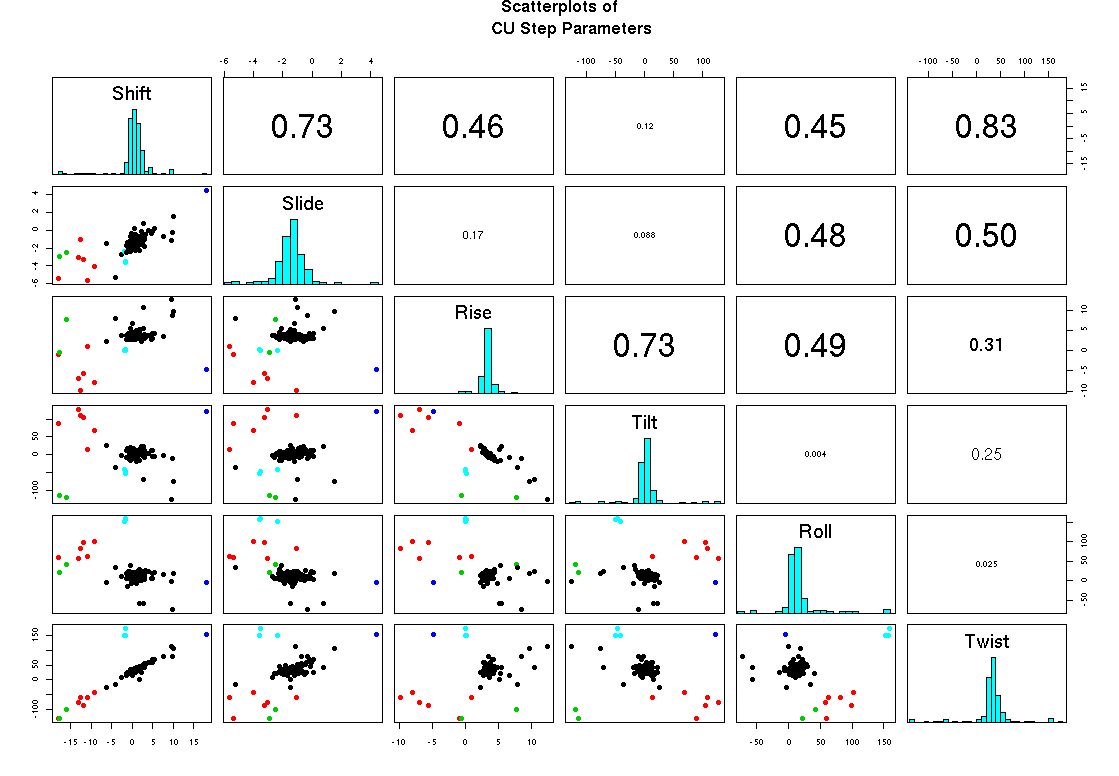
\includegraphics[angle=90, scale=0.6]{All/CU.png}
\caption{Scatterplots for step-parameters of \textbf{All} CU dinucleotide steps
in 50S rRNA.}
\label{fig:stepsCU}
\end{figure}

\begin{figure}[H]
\centering
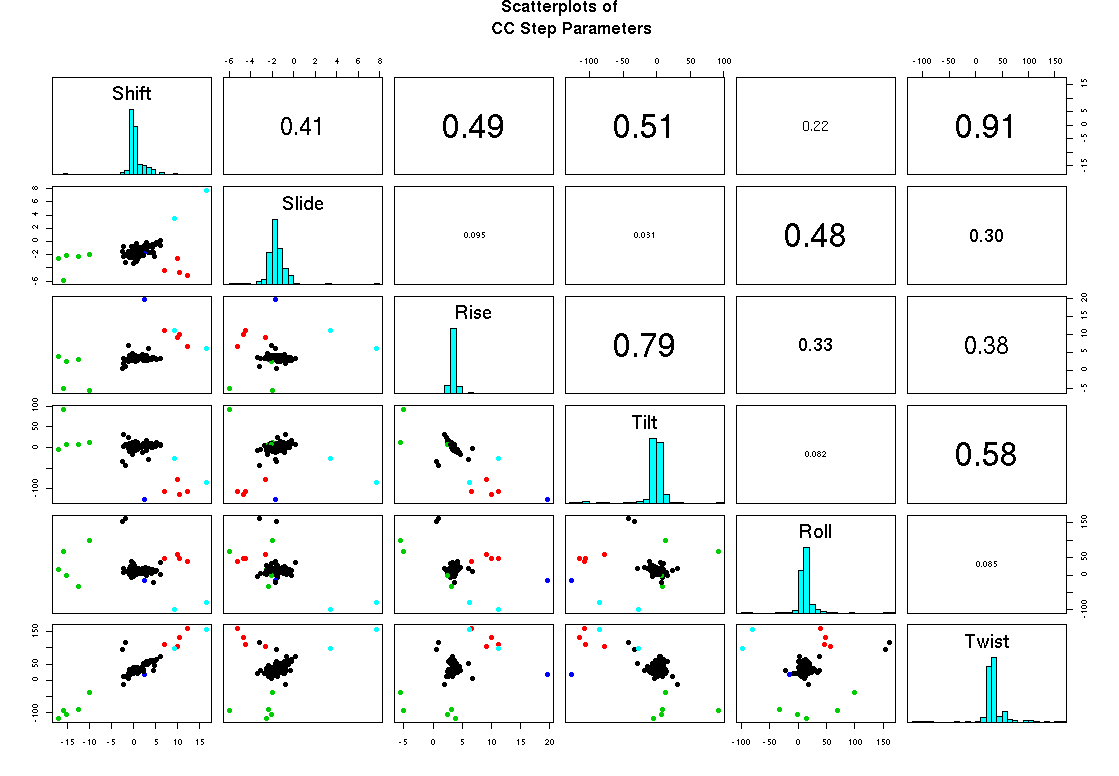
\includegraphics[angle=90, scale=0.6]{All/CC.png}
\caption{Scatterplots for step-parameters of \textbf{All} CC dinucleotide steps
in 50S rRNA.}
\label{fig:stepsCC}
\end{figure}

\begin{figure}[H]
\centering
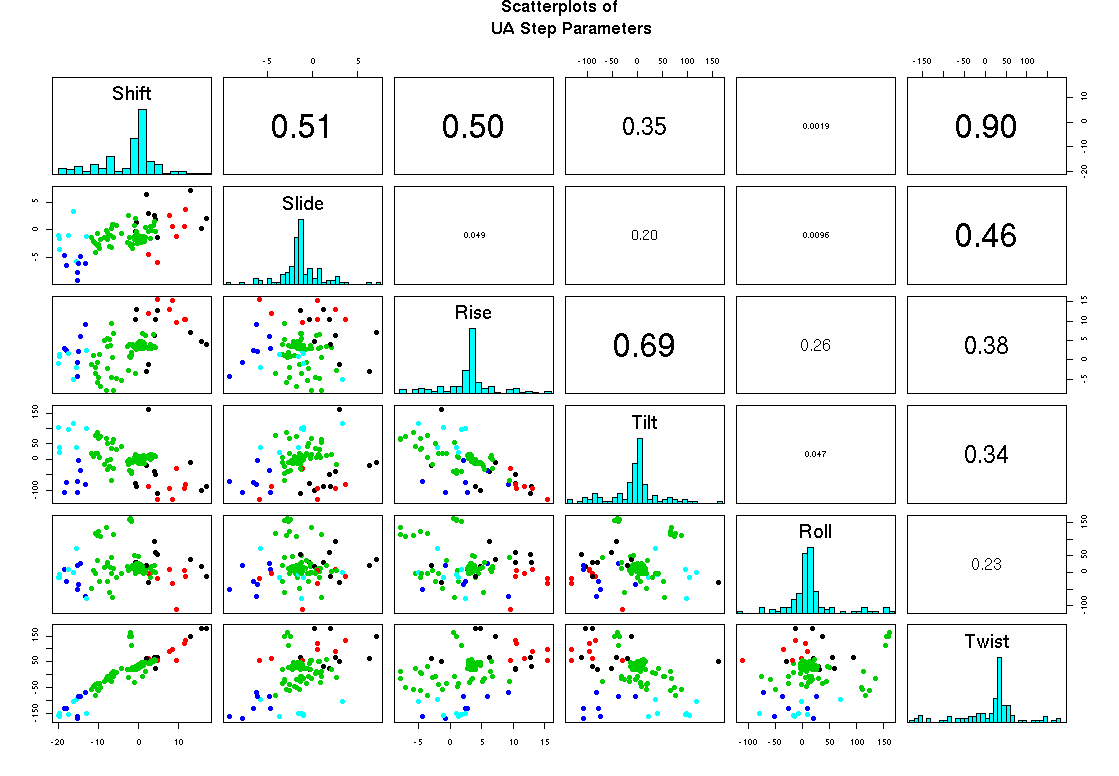
\includegraphics[angle=90, scale=0.6]{All/UA.png}
\caption{Scatterplots for step-parameters of \textbf{All} UA dinucleotide steps
in 50S rRNA.}
\label{fig:stepsUA}
\end{figure}

\begin{figure}[H]
\centering
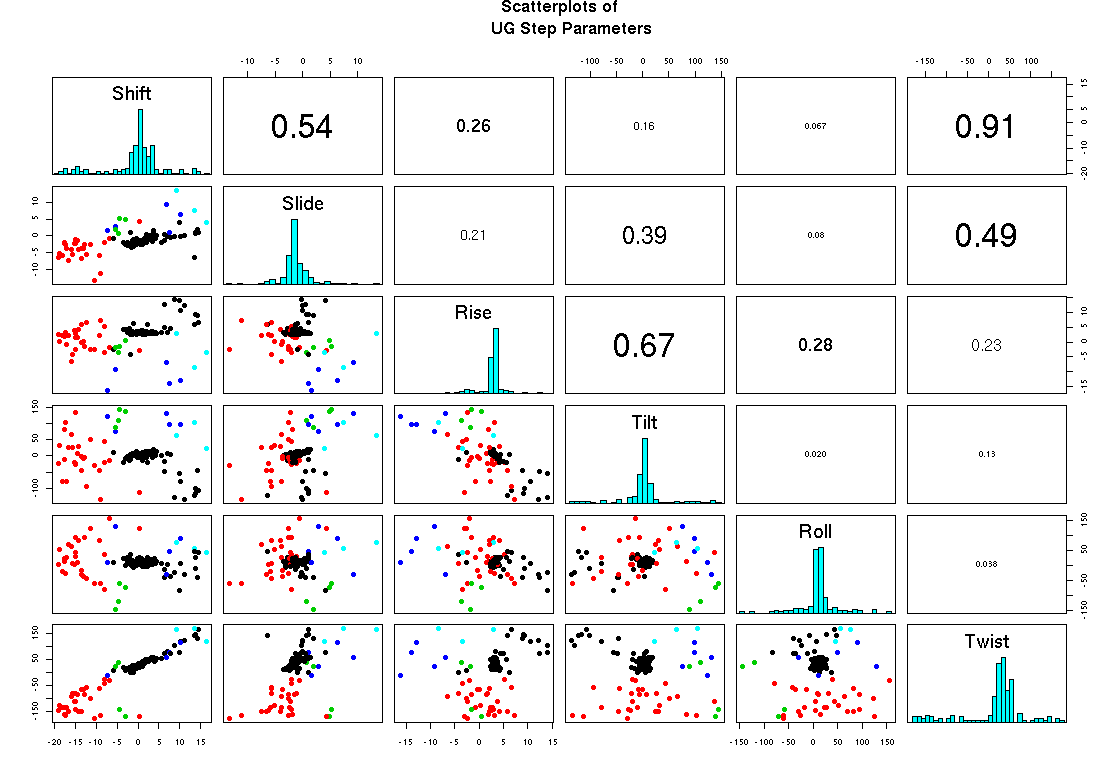
\includegraphics[angle=90, scale=0.6]{All/UG.png}
\caption{Scatterplots for step-parameters of \textbf{All} UG dinucleotide steps
in 50S rRNA.}
\label{fig:stepsUG}
\end{figure}

\begin{figure}[H]
\centering
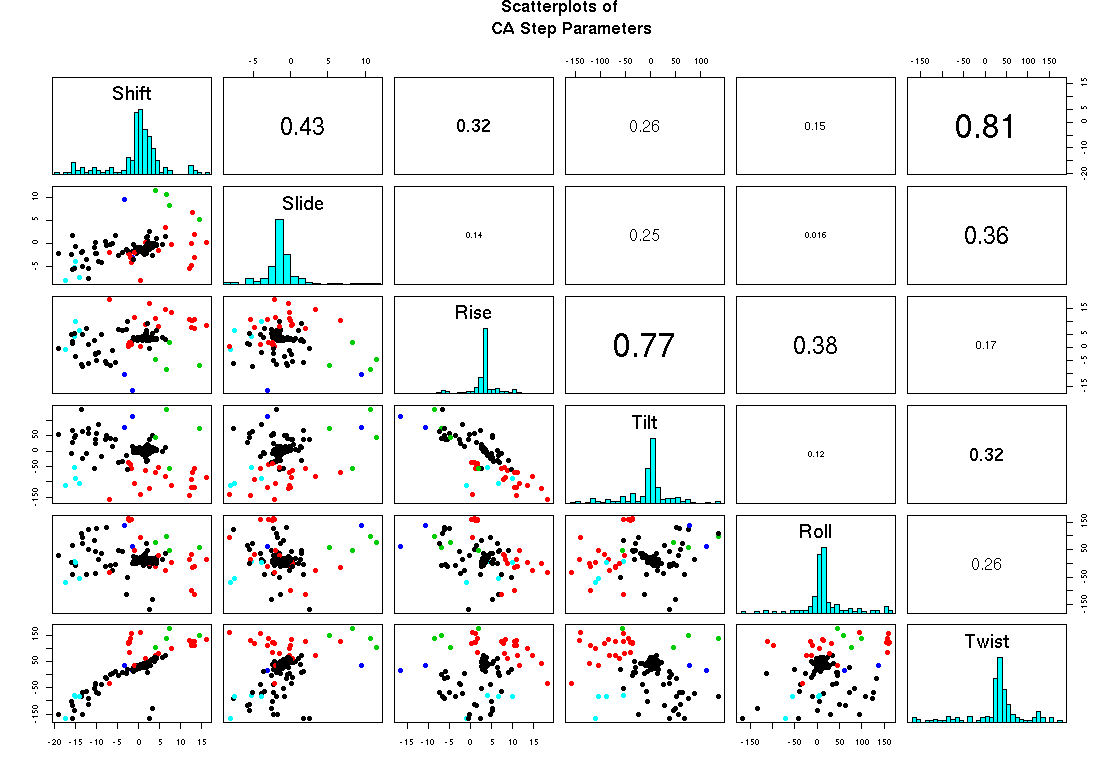
\includegraphics[angle=90, scale=0.6]{All/CA.png}
\caption{Scatterplots for step-parameters of \textbf{All} CA dinucleotide steps
in 50S rRNA.}
\label{fig:stepsCA}
\end{figure}

\begin{figure}[H]
\centering
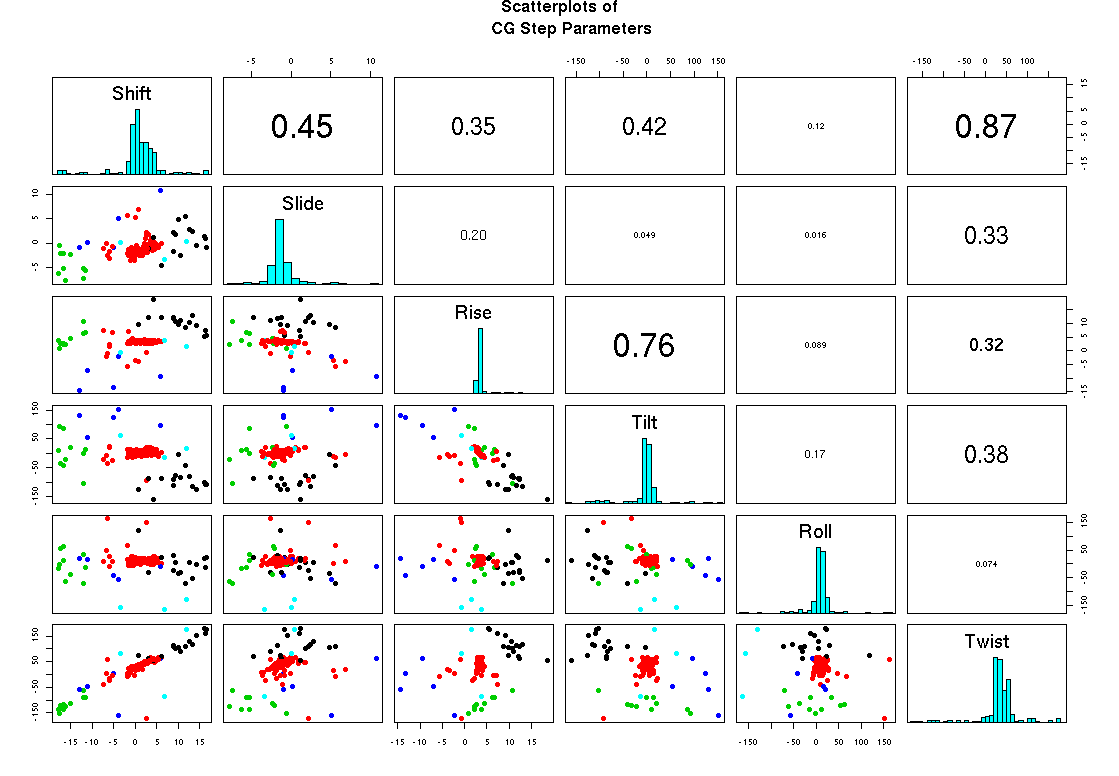
\includegraphics[angle=90, scale=0.6]{All/CG.png}
\caption{Scatterplots for step-parameters of \textbf{All} CG dinucleotide steps
in 50S rRNA.}
\label{fig:stepsCG}
\end{figure}

\begin{figure}[H]
\centering
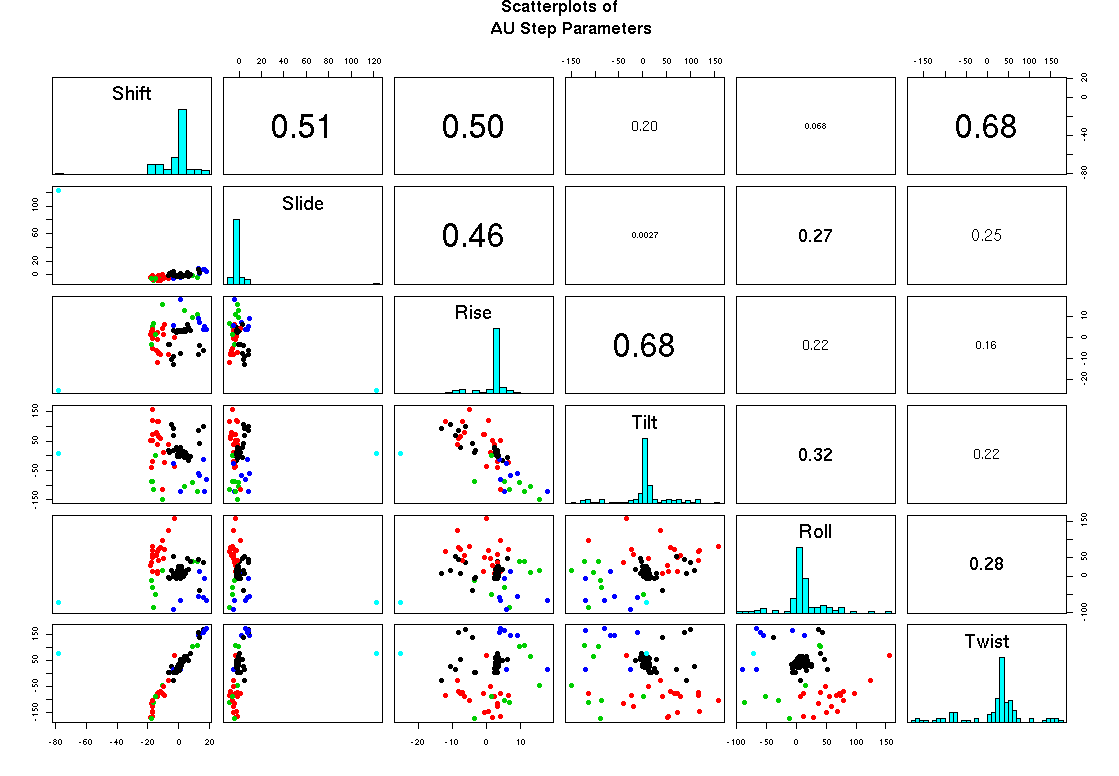
\includegraphics[angle=90, scale=0.6]{All/AU.png}
\caption{Scatterplots for step-parameters of \textbf{All} AU dinucleotide steps
in 50S rRNA.}
\label{fig:stepsAU}
\end{figure}

\begin{figure}[H]
\centering
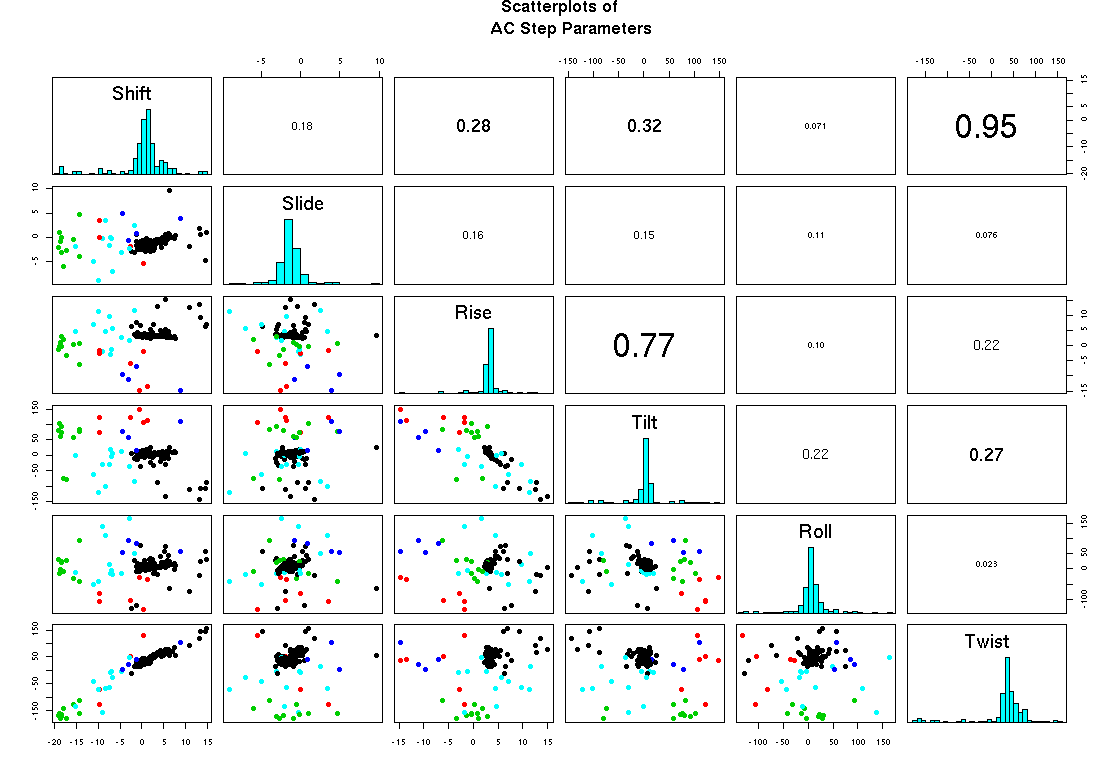
\includegraphics[angle=90, scale=0.6]{All/AC.png}
\caption{Scatterplots for step-parameters of \textbf{All} AC dinucleotide steps
in 50S rRNA.}
\label{fig:stepsAC}
\end{figure}

\begin{figure}[H]
\centering
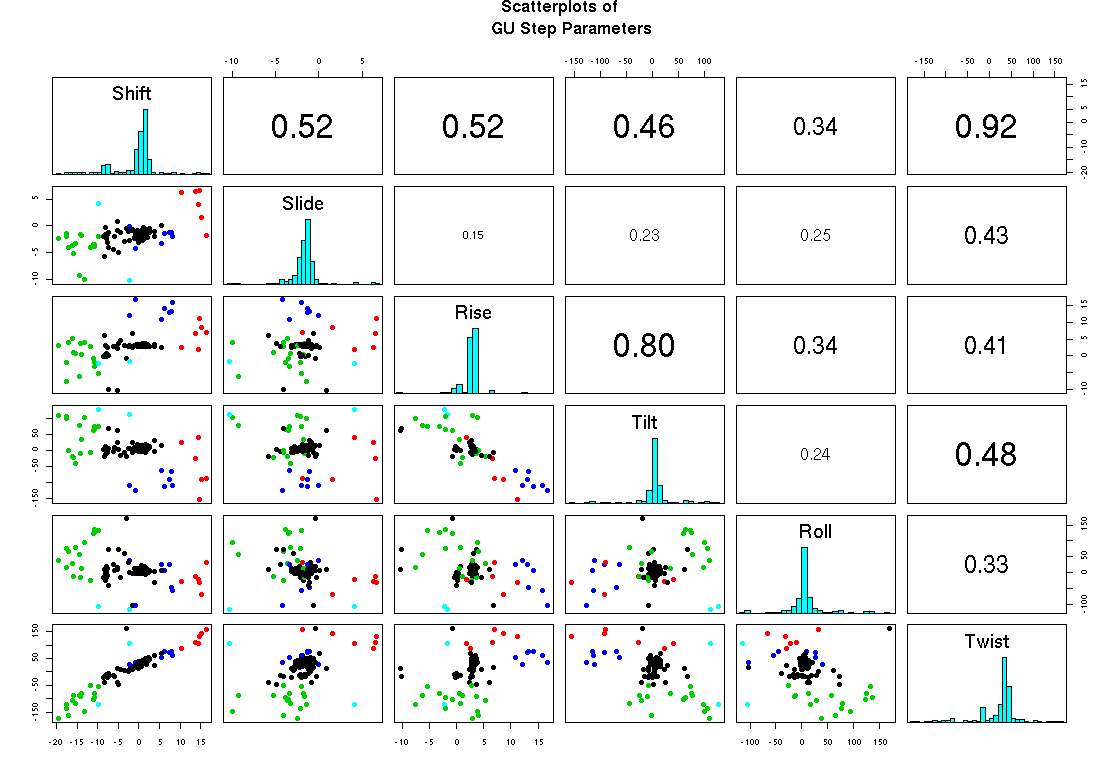
\includegraphics[angle=90, scale=0.6]{All/GU.png}
\caption{Scatterplots for step-parameters of \textbf{All} GU dinucleotide steps
in 50S rRNA.}
\label{fig:stepsGU}
\end{figure}

\begin{figure}[H]
\centering
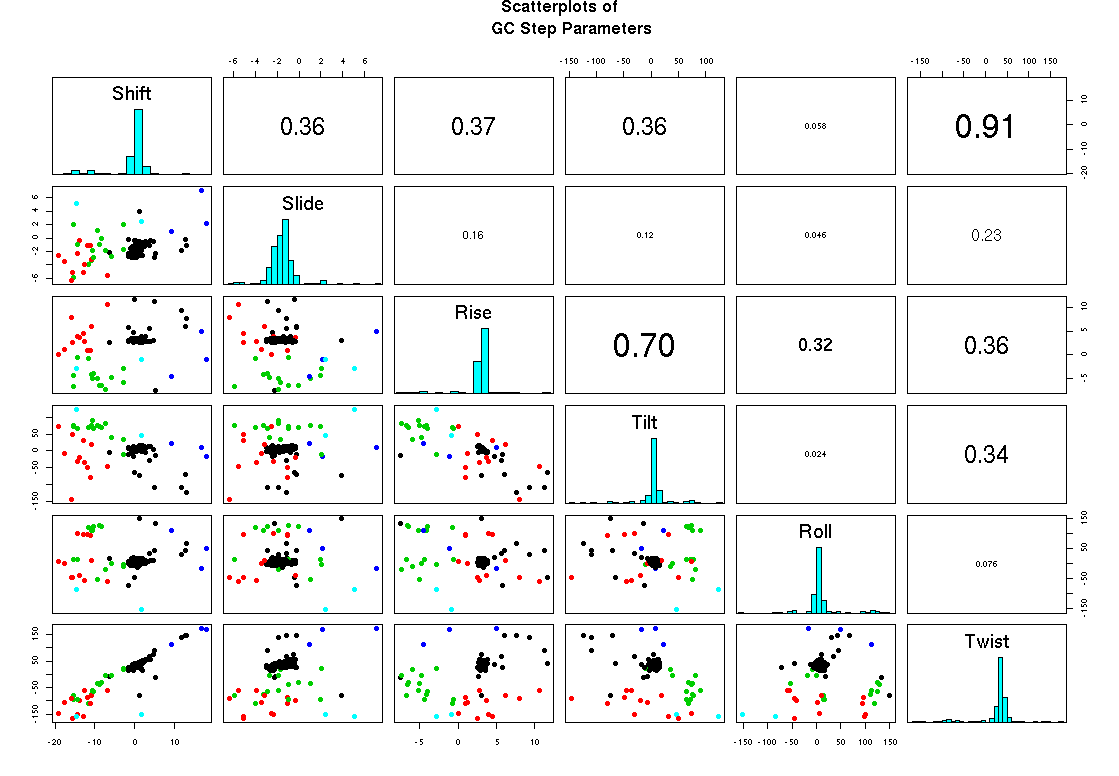
\includegraphics[angle=90, scale=0.6]{All/GC.png}
\caption{Scatterplots for step-parameters of \textbf{All} GC dinucleotide steps
in 50S rRNA.}
\label{fig:stepsGC}
\end{figure}

%%%%%%%%%%%%%%%%%%%%%%%%%%%%%%%%%%%%%%%%%%%%%%%%%
%THE FOLLOWING ARE THE SCATTERPLOTS FOR HELICAL STEPS
%%%%%%%%%%%%%%%%%%%%%%%%%%%%%%%%%%%%%%%%%%%%%%%%

\begin{figure}[H]
\centering
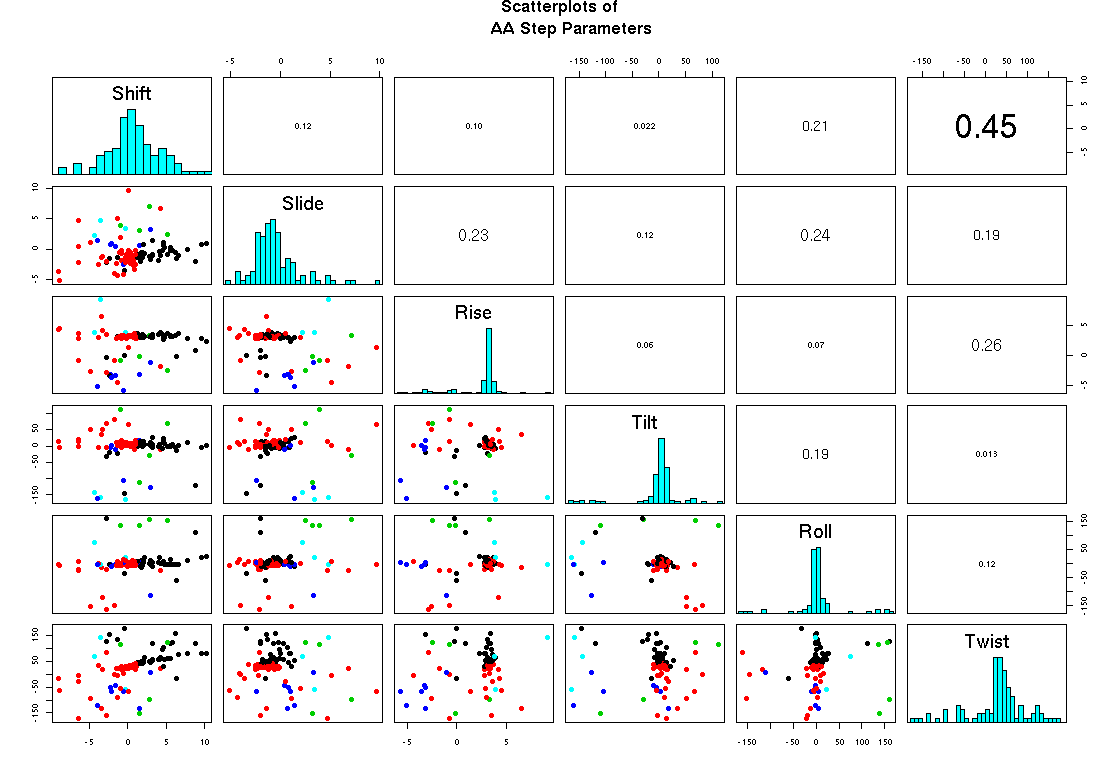
\includegraphics[angle=90, scale=0.6]{Helical/AA.png}
\caption{Scatterplots for step-parameters of \textbf{Helical} AA dinucleotide steps
in 50S rRNA.}
\label{fig:stepsAA}
\end{figure}

\begin{figure}[H]
\centering
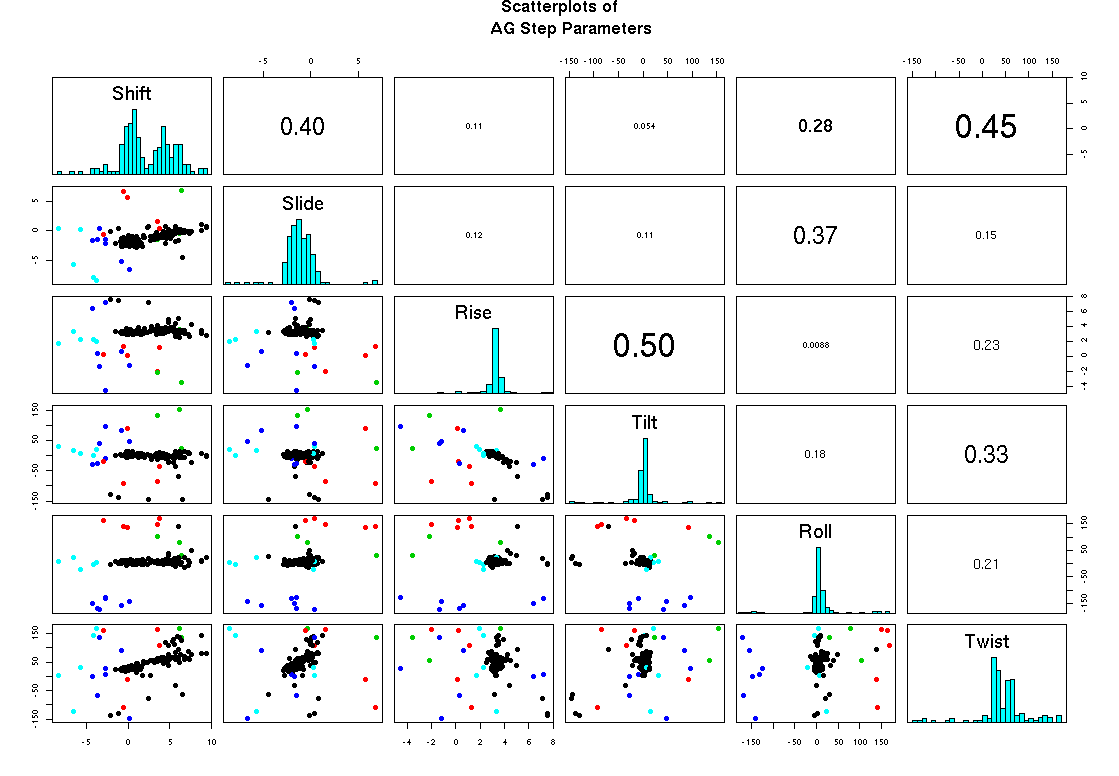
\includegraphics[angle=90, scale=0.6]{Helical/AG.png}
\caption{Scatterplots for step-parameters of \textbf{Helical} AG dinucleotide steps
in 50S rRNA.}
\label{fig:stepsAG}
\end{figure}

\begin{figure}[H]
\centering
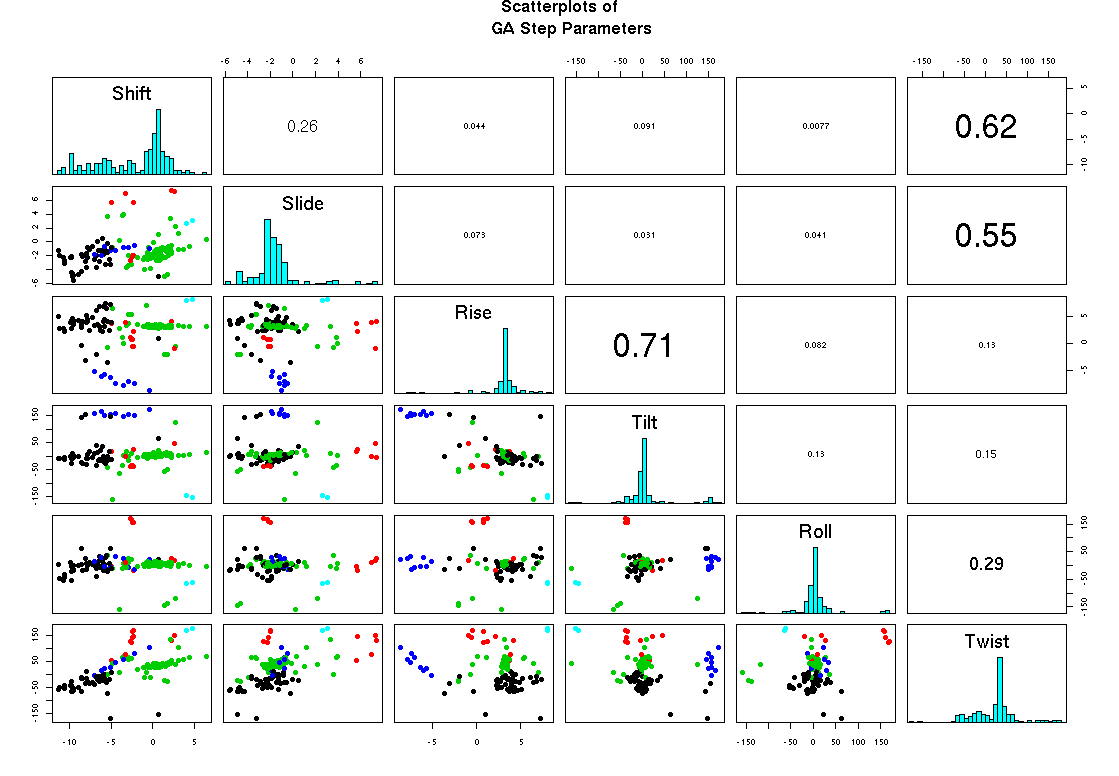
\includegraphics[angle=90, scale=0.6]{Helical/GA.png}
\caption{Scatterplots for step-parameters of \textbf{Helical} GA dinucleotide steps
in 50S rRNA.}
\label{fig:stepsGA}
\end{figure}

\begin{figure}[H]
\centering
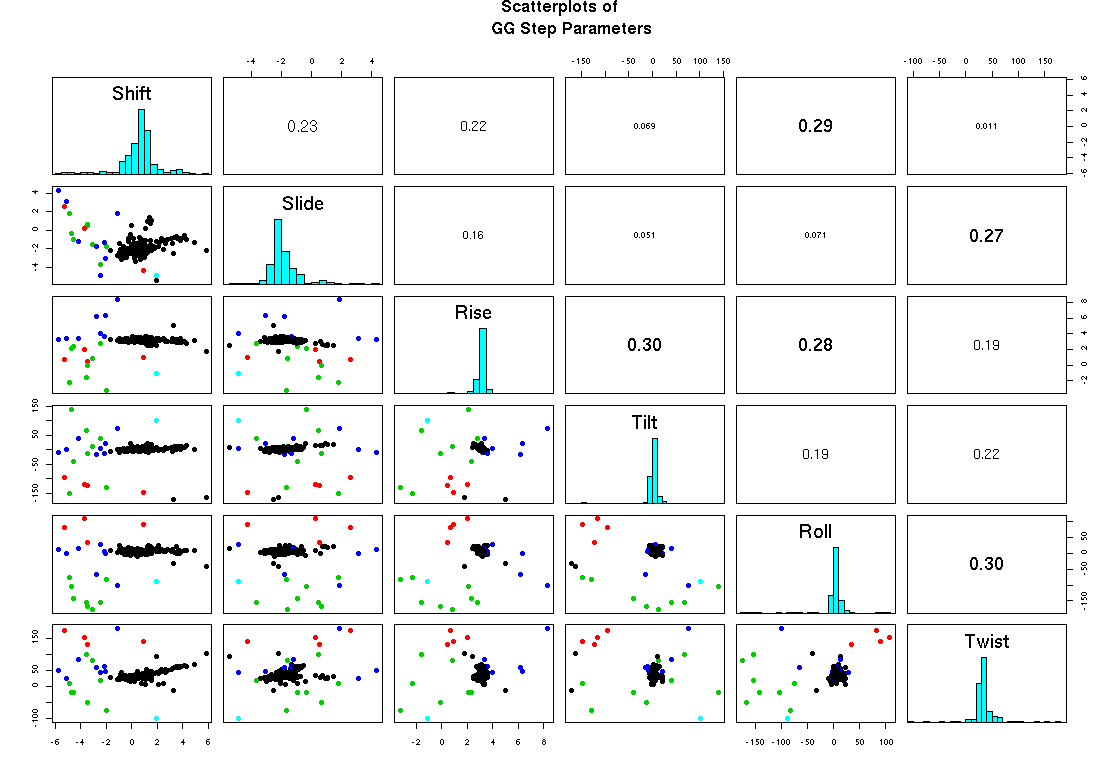
\includegraphics[angle=90, scale=0.6]{Helical/GG.png}
\caption{Scatterplots for step-parameters of \textbf{Helical} GG dinucleotide steps
in 50S rRNA.}
\label{fig:stepsGG}
\end{figure}

\begin{figure}[H]
\centering
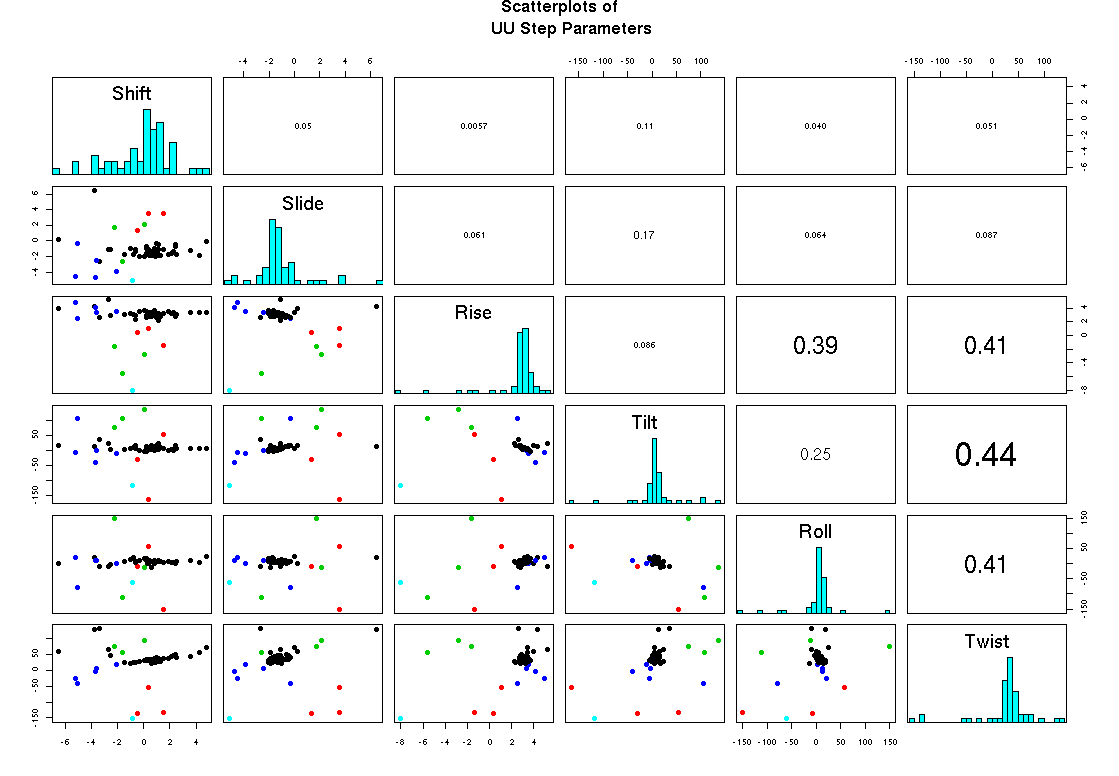
\includegraphics[angle=90, scale=0.6]{Helical/UU.png}
\caption{Scatterplots for step-parameters of \textbf{Helical} UU dinucleotide steps
in 50S rRNA.}
\label{fig:stepsUU}
\end{figure}

\begin{figure}[H]
\centering
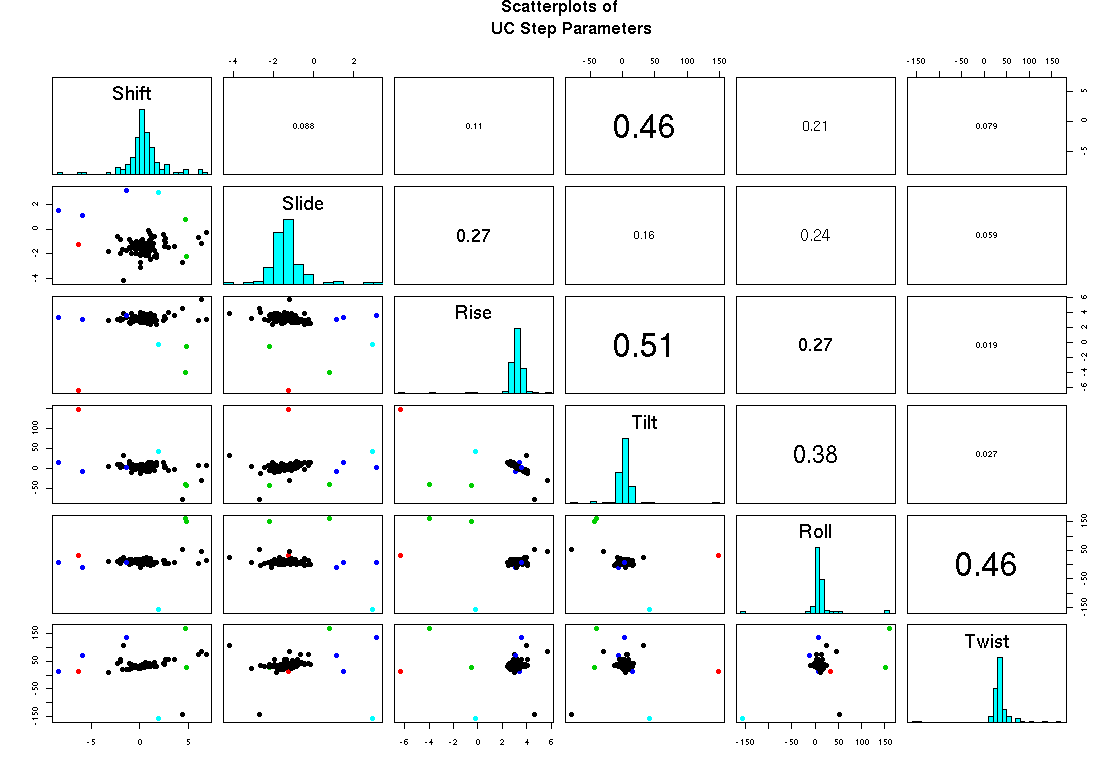
\includegraphics[angle=90, scale=0.6]{Helical/UC.png}
\caption{Scatterplots for step-parameters of \textbf{Helical} UC dinucleotide steps
in 50S rRNA.}
\label{fig:stepsUC}
\end{figure}

\begin{figure}[H]
\centering
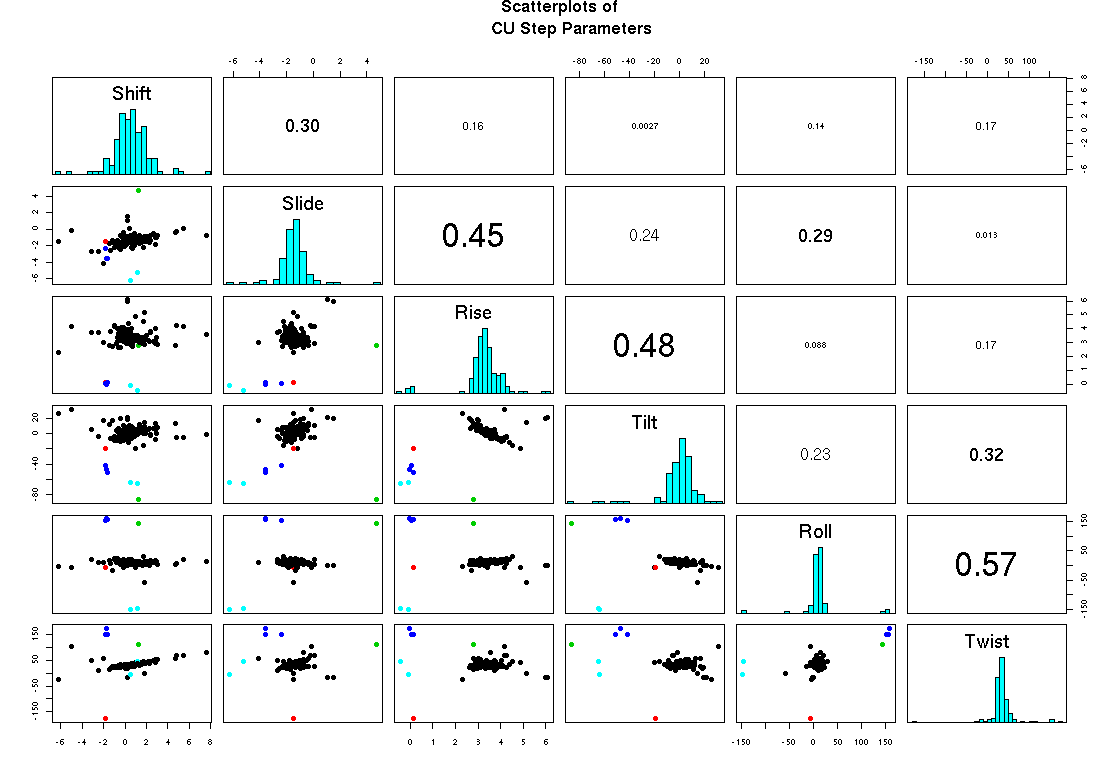
\includegraphics[angle=90, scale=0.6]{Helical/CU.png}
\caption{Scatterplots for step-parameters of \textbf{Helical} CU dinucleotide steps
in 50S rRNA.}
\label{fig:stepsCU}
\end{figure}

\begin{figure}[H]
\centering
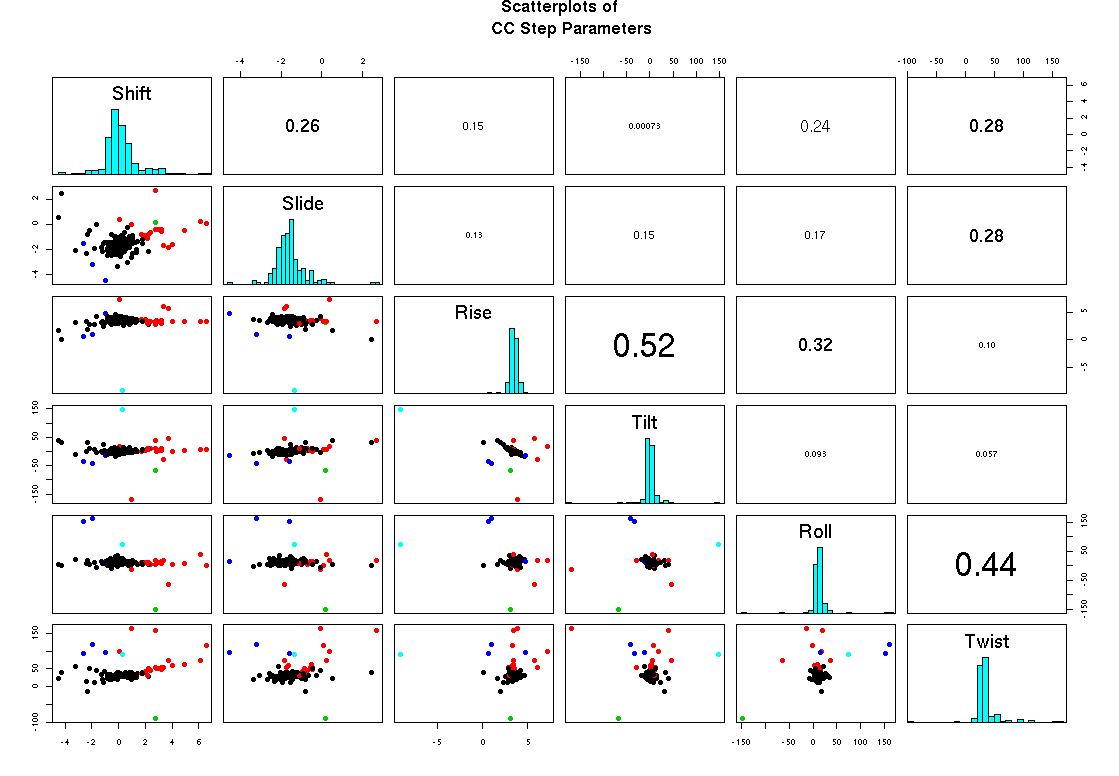
\includegraphics[angle=90, scale=0.6]{Helical/CC.png}
\caption{Scatterplots for step-parameters of \textbf{Helical} CC dinucleotide steps
in 50S rRNA.}
\label{fig:stepsCC}
\end{figure}

\begin{figure}[H]
\centering
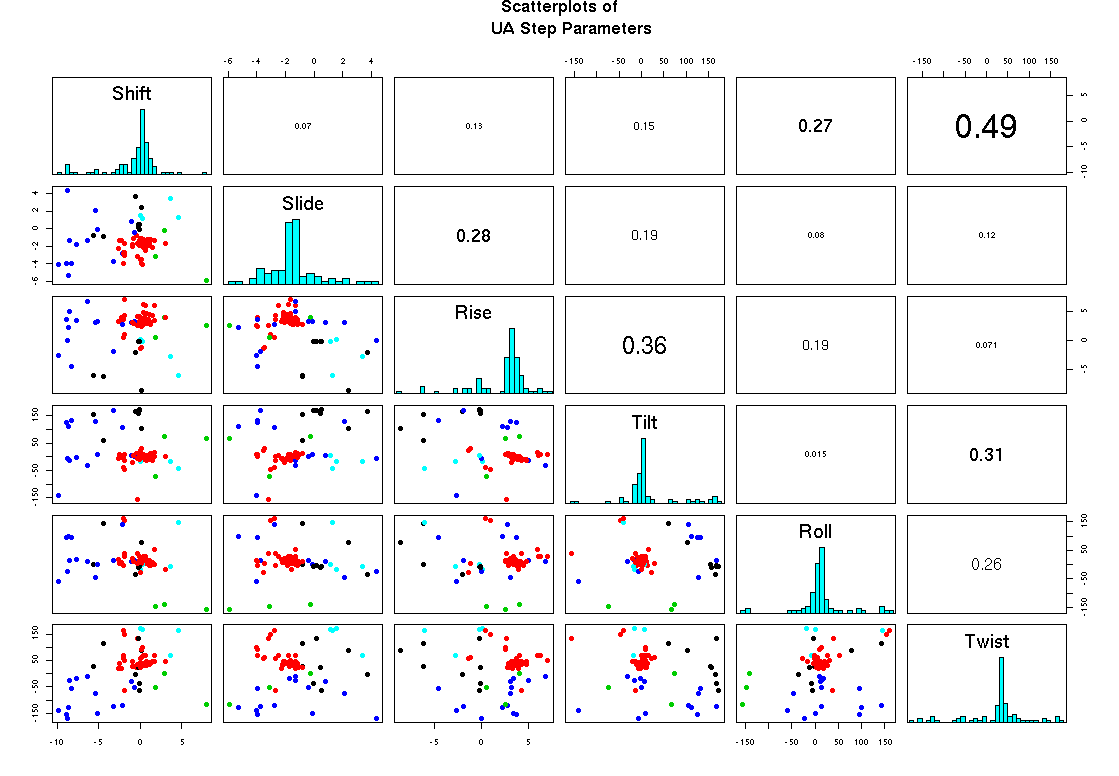
\includegraphics[angle=90, scale=0.6]{Helical/UA.png}
\caption{Scatterplots for step-parameters of \textbf{Helical} UA dinucleotide steps
in 50S rRNA.}
\label{fig:stepsUA}
\end{figure}

\begin{figure}[H]
\centering
\includegraphics[angle=90, scale=0.6]{Helical/UG.png}
\caption{Scatterplots for step-parameters of \textbf{Helical} UG dinucleotide steps
in 50S rRNA.}
\label{fig:stepsUG}
\end{figure}

\begin{figure}[H]
\centering
\includegraphics[angle=90, scale=0.6]{Helical/CA.png}
\caption{Scatterplots for step-parameters of \textbf{Helical} CA dinucleotide steps
in 50S rRNA.}
\label{fig:stepsCA}
\end{figure}

\begin{figure}[H]
\centering
\includegraphics[angle=90, scale=0.6]{Helical/CG.png}
\caption{Scatterplots for step-parameters of \textbf{Helical} CG dinucleotide steps
in 50S rRNA.}
\label{fig:stepsCG}
\end{figure}

\begin{figure}[H]
\centering
\includegraphics[angle=90, scale=0.6]{Helical/AU.png}
\caption{Scatterplots for step-parameters of \textbf{Helical} AU dinucleotide steps
in 50S rRNA.}
\label{fig:stepsAU}
\end{figure}

\begin{figure}[H]
\centering
\includegraphics[angle=90, scale=0.6]{Helical/AC.png}
\caption{Scatterplots for step-parameters of \textbf{Helical} AC dinucleotide steps
in 50S rRNA.}
\label{fig:stepsAC}
\end{figure}

\begin{figure}[H]
\centering
\includegraphics[angle=90, scale=0.6]{Helical/GU.png}
\caption{Scatterplots for step-parameters of \textbf{Helical} GU dinucleotide steps
in 50S rRNA.}
\label{fig:stepsGU}
\end{figure}

\begin{figure}[H]
\centering
\includegraphics[angle=90, scale=0.6]{Helical/GC.png}
\caption{Scatterplots for step-parameters of \textbf{Helical} GC dinucleotide steps
in 50S rRNA.}
\label{fig:stepsGC}
\end{figure}

%%%%%%%%%%%%%%%%%%%%%%%%%%%%%%%%%%%%%%%%%%%%%%%%%
%THE FOLLOWING ARE THE SCATTERPLOTS FOR WC STEPS
%%%%%%%%%%%%%%%%%%%%%%%%%%%%%%%%%%%%%%%%%%%%%%%%

\begin{figure}[H]
\centering
\includegraphics[angle=90, scale=0.6]{WC/AA.png}
\caption{Scatterplots for step-parameters of \textbf{WC} AA dinucleotide steps
in 50S rRNA.}
\label{fig:stepsAA}
\end{figure}

\begin{figure}[H]
\centering
\includegraphics[angle=90, scale=0.6]{WC/AG.png}
\caption{Scatterplots for step-parameters of \textbf{WC} AG dinucleotide steps
in 50S rRNA.}
\label{fig:stepsAG}
\end{figure}

\begin{figure}[H]
\centering
\includegraphics[angle=90, scale=0.6]{WC/GA.png}
\caption{Scatterplots for step-parameters of \textbf{WC} GA dinucleotide steps
in 50S rRNA.}
\label{fig:stepsGA}
\end{figure}

\begin{figure}[H]
\centering
\includegraphics[angle=90, scale=0.6]{WC/GG.png}
\caption{Scatterplots for step-parameters of \textbf{WC} GG dinucleotide steps
in 50S rRNA.}
\label{fig:stepsGG}
\end{figure}

\begin{figure}[H]
\centering
\includegraphics[angle=90, scale=0.6]{WC/UU.png}
\caption{Scatterplots for step-parameters of \textbf{WC} UU dinucleotide steps
in 50S rRNA.}
\label{fig:stepsUU}
\end{figure}

\begin{figure}[H]
\centering
\includegraphics[angle=90, scale=0.6]{WC/UC.png}
\caption{Scatterplots for step-parameters of \textbf{WC} UC dinucleotide steps
in 50S rRNA.}
\label{fig:stepsUC}
\end{figure}

\begin{figure}[H]
\centering
\includegraphics[angle=90, scale=0.6]{WC/CU.png}
\caption{Scatterplots for step-parameters of \textbf{WC} CU dinucleotide steps
in 50S rRNA.}
\label{fig:stepsCU}
\end{figure}

\begin{figure}[H]
\centering
\includegraphics[angle=90, scale=0.6]{WC/CC.png}
\caption{Scatterplots for step-parameters of \textbf{WC} CC dinucleotide steps
in 50S rRNA.}
\label{fig:stepsCC}
\end{figure}

\begin{figure}[H]
\centering
\includegraphics[angle=90, scale=0.6]{WC/UA.png}
\caption{Scatterplots for step-parameters of \textbf{WC} UA dinucleotide steps
in 50S rRNA.}
\label{fig:stepsUA}
\end{figure}

\begin{figure}[H]
\centering
\includegraphics[angle=90, scale=0.6]{WC/UG.png}
\caption{Scatterplots for step-parameters of \textbf{WC} UG dinucleotide steps
in 50S rRNA.}
\label{fig:stepsUG}
\end{figure}

\begin{figure}[H]
\centering
\includegraphics[angle=90, scale=0.6]{WC/CA.png}
\caption{Scatterplots for step-parameters of \textbf{WC} CA dinucleotide steps
in 50S rRNA.}
\label{fig:stepsCA}
\end{figure}

\begin{figure}[H]
\centering
\includegraphics[angle=90, scale=0.6]{WC/CG.png}
\caption{Scatterplots for step-parameters of \textbf{WC} CG dinucleotide steps
in 50S rRNA.}
\label{fig:stepsCG}
\end{figure}

\begin{figure}[H]
\centering
\includegraphics[angle=90, scale=0.6]{WC/AU.png}
\caption{Scatterplots for step-parameters of \textbf{WC} AU dinucleotide steps
in 50S rRNA.}
\label{fig:stepsAU}
\end{figure}

\begin{figure}[H]
\centering
\includegraphics[angle=90, scale=0.6]{WC/AC.png}
\caption{Scatterplots for step-parameters of \textbf{WC} AC dinucleotide steps
in 50S rRNA.}
\label{fig:stepsAC}
\end{figure}

\begin{figure}[H]
\centering
\includegraphics[angle=90, scale=0.6]{WC/GU.png}
\caption{Scatterplots for step-parameters of \textbf{WC} GU dinucleotide steps
in 50S rRNA.}
\label{fig:stepsGU}
\end{figure}

\begin{figure}[H]
\centering
\includegraphics[angle=90, scale=0.6]{WC/GC.png}
\caption{Scatterplots for step-parameters of \textbf{WC} GC dinucleotide steps
in 50S rRNA.}
\label{fig:stepsGC}
\end{figure}

%\section{}

%\bibliography{biblio}
\printindex

    \chapter{RNA Dataset}
\bibliographystyle{nar}
%\bibliographystyle{jacs}
\label{clustering} 
MicroRNAs (miRNA) are small (~22 nucleotide) helical RNA's which
down-regulate translation in Eukaryotes forming partial duplex
structures with mRNA \cite{ruvkun2001}. Motivated by the goal of
understanding the structural role non-canonical base pairs play in the regulatory
mechanisms in which miRNAs take part, we have assembled a data set of
785 RNA crystal structures taken from the Protein Data Bank (PDB). The
collected structures are composed of a minimum of 3 base pairs, have
been parsed through 3DNA to detect hydrogen bonds with a distance no
longer than $3.4$ \AA, Stagger $ \le 1.5$ \AA, Buckle $ \le 30^{\circ}$, and
other 3DNA parameters in their default values.

\section{Base Pair Counting and Classification}
\setlongtables
%\begin{table}[H]
\begin{center}
%{\small
%\begin{tabular}{c|p{5cm}|c|c|c}
\begin{longtable}{l|c}
\caption{Distribution of BP (Base Pairs) in RNA Database with 785
  Crystal Structures.} \label{tab:all}\\
\hline
Total number of base pairs & 131934   \\ \hline
Total number of WC base pairs & 87735(66.5\%)   \\ \hline
Total number of non-WC base pairs & 44199(33.5\%)  \\ \hline
\end{longtable}
%}
\end{center}
%\end{table}

In Figure~\ref{fig:WCandnon} we show a scatterplot for the base pair parameters of WC 
base pairs in red, and non-WC base pairs in blue. From this Figure
it's clear that WC base pairs have a narrow distribution for Shear, Stretch and Opening, 
but for Stagger, Buckle and Propeller, the distribution is almost as broad as that of
non-cannonical WC base pairs. Taking this fact into account we can now
split our dataset in two parts, a WC one, and a non-canonical one.

\begin{figure}[H]
\centering
\includegraphics[scale=0.6, angle=90]{allscatter.png}
\caption{Scatterplots showing the distribution of Watson-Crick (WC)
  and Non-WC base pair in dataset.}
\label{fig:WCandnon}
\end{figure}


\subsection{Watson-Crick and non-canonical Base Pairs}

\begin{center}
\begin{longtable}{c|c}
\caption{Distribution of base pairs according to Leontis-Westhof (LW) classification.}\\ \hline
\bf{Number of Base Pairs} & \bf{LW Clasification} \\ \hline \hline
 105703 & cis-W/W     \\ \hline
   9570 & NA          \\ \hline
   4158 & trans-S/H   \\ \hline
   3101 & trans-H/S   \\ \hline
   2593 & trans-W/H   \\ \hline
   1926 & trans-H/W   \\ \hline
   1050 & trans-W/W   \\ \hline
    691 & trans-H/H   \\ \hline
    677 & trans-S/W   \\ \hline
    566 & cis-W/H     \\ \hline
    431 & cis-W/S     \\ \hline
    371 & cis-S/W     \\ \hline
    333 & cis-H/W     \\ \hline
    195 & trans-W/S   \\ \hline
    178 & cis-S/H     \\ \hline
    132 & trans-S/S   \\ \hline
    117 & cis-H/S     \\ \hline
     82 & cis-S/S     \\ \hline
     23 & cis-H/H     \\ \hline
     11 & trans-W/.   \\ \hline
      5 & cis-X/X     \\ \hline
      5 & cis-W/.     \\ \hline
      5 & cis-H/.     \\ \hline
      3 & trans-./W   \\ \hline
      3 & trans-S/.   \\ \hline
      3 & trans-./S   \\ \hline
      1 & trans-./H   \\ \hline
      1 & cis-./.     \\ \hline
\end{longtable}
\end{center}


\subsection{Watson-Crick Base Pairs}

In addition to Figure~\ref{fig:WCandnon} we have also colored the most
abundant WC base pairs  in Figure~\ref{fig:mainWC} that is, CG, GC, AU, and UA, base
pairs. The base pairs counts for every possible Watson-Crick pair can
be seen in Table~\ref{tab:allWC}, and the average base pair parameters
and their standard deviations can be seen in Table~\ref{tab:WCave}

\begin{figure}[H]
\centering
\includegraphics[scale=0.6, angle=90]{CGGCAUUA.png}
\caption{Scatterplots showing the distribution of Watson-Crick (WC)
  base pairs colored as CG(Cyan), GC(Green), AU(Blue), UA(Red), others(black)}
\label{fig:mainWC}
\end{figure}


\begin{center}
\begin{longtable}{c|c}
\caption{Number of WC base pairs sorted by base pair ID.}
\label{tab:allWC}\\ 
%This is the header for the first page of the table...
\hline \hline 
\bf{Number of Base Pairs} & \bf{Base Pair Type} \\\hline
\endfirsthead

%This is the header for the remaining page(s) of the table...
\multicolumn{1}{c}{{\tablename} \thetable{} -- Continued} \\
\hline \hline 
\bf{Number of Base Pairs} & \bf{Base Pair Type} \\\hline
\endhead

%This is the footer for all pages except the last page of the table...
\multicolumn{1}{l}{Continued on Next Page\ldots} \\
\endfoot
%This is the footer for the last page of the table...
\endlastfoot
  33036 & C:G      \\ \hline
  31216 & G:C      \\ \hline
  11756 & A:U      \\ \hline
  11424 & U:A      \\ \hline
     61 & 5MC:G    \\ \hline
     35 & 5BU:A    \\ \hline
     24 & 2MG:C    \\ \hline
     20 & A:5BU    \\ \hline
     16 & G48:C43  \\ \hline
     12 & C43:G48  \\ \hline
     11 & OMG:OMC  \\ \hline
      9 & OMC:OMG  \\ \hline
      8 & U36:A44  \\ \hline
      8 & DC:G     \\ \hline
      8 & A44:U36  \\ \hline
      7 & LC:LG    \\ \hline
      7 & G:CBV    \\ \hline
      6 & G:5MC    \\ \hline
      6 & CBV:G    \\ \hline
      5 & CBR:G    \\ \hline
      4 & UMS:A    \\ \hline
      4 & LG:LC    \\ \hline
      4 & GTP:C    \\ \hline
      4 & G:CBR    \\ \hline
      4 & CSL:G    \\ \hline
      4 & 52:22    \\ \hline
      3 & IU:A     \\ \hline
      3 & C:2MG    \\ \hline
      2 & G:5IC    \\ \hline
      2 & C:GTP    \\ \hline
      2 & A:IU     \\ \hline
      2 & 5CG:C    \\ \hline
      1 & U:RIA    \\ \hline
      1 & SSU:A    \\ \hline
      1 & S4C:G    \\ \hline
      1 & OMU:A2M  \\ \hline
      1 & N5C:G    \\ \hline
      1 & G:S4C    \\ \hline
      1 & G:CSL    \\ \hline
      1 & G:CB2    \\ \hline
      1 & G:A5M    \\ \hline
      1 & G:74     \\ \hline
      1 & DG:C     \\ \hline
      1 & DA:U     \\ \hline
      1 & C:XUG    \\ \hline
      1 & CTP:G    \\ \hline
      1 & C:DG     \\ \hline
      1 & CB2:G    \\ \hline
      1 & C:7MG    \\ \hline
      1 & ADE:74   \\ \hline
      1 & A5M:G    \\ \hline
      1 & A2M:OMU  \\ \hline
      1 & 47:56    \\ \hline
      1 & 1SC:G    \\ \hline 
\end{longtable}
\end{center}

\begin{center}
{\small
\begin{longtable}{c|c|c|c|c|c|c}
\caption{\normalsize{This table summarizes for Watson-Crick base pairs, the base
  pair parameters average values with standard  deviations in
  parentheses.}} \label{tab:WCave}\\ 
\hline
\parbox[t]{1.8cm}{\bf{Base Pair Parameter}} & \bf{CG} & \bf{GC} & \bf{AU} & \bf{UA} & \bf{others} & \bf{ARNA}\\ \hline \hline
Shear     &  0.169(0.311)  & -0.184(0.315) &  0.035(0.276)  & -0.034(0.292) & -0.070(0.381) &  0.01 \\ \hline
Stretch   & -0.149(0.135)  & -0.148(0.132) & -0.122(0.118)  & -0.121(0.120) & -0.175(0.151) & -0.08 \\ \hline
Stagger   & -0.145(0.427)  & -0.138(0.407) & -0.042(0.394)  & -0.046(0.391) &  0.001(0.285) &  0.01 \\ \hline
Buckle    &  3.888(9.589)  & -3.631(9.446) & -0.817(8.750)  &  1.209(8.700) &  0.688(6.590) & -0.00 \\ \hline
Propeller & -6.568(8.841)  & -6.309(8.721) & -4.724(10.537) & -6.350(8.672) & -9.678(7.052) & -2.07 \\ \hline
Opening   &  0.454(3.600)  &  0.509(3.643) &  0.709(5.349)  &
1.043(5.248) &  3.554(0.313) & -1.67 \\ \hline 
\end{longtable}

}
\end{center}

As can be seen in Table~\ref{tab:LW} all CG, GC, AU, and UA cannonical
base pairs are given the cis-W/W LW classification, or are classified
as NA as is expected.

\begin{center}
\begin{longtable}{c|c|c}
\caption{Canonical WC Base-Pairs in dataset.}
\label{tab:LW}\\
\hline
\bf{Number of Base Pairs} & \bf{Base Pair Type} & \bf{LW Classification} \\ \hline \hline
  31680 & C:G & cis-W/W  \\ \hline
  29908 & G:C & cis-W/W  \\ \hline
  11435 & A:U & cis-W/W  \\ \hline
  11089 & U:A & cis-W/W  \\ \hline
   1356 & C:G & NA       \\ \hline
   1308 & G:C & NA       \\ \hline
    335 & U:A & NA       \\ \hline
    321 & A:U & NA       \\ \hline
\end{longtable}

\end{center}

       
\begin{center}
\begin{longtable}{c|c|c|c}
\hline
\bf{Number of Base Pairs} & \bf{Base Pair Type} & \bf{Helical Classification} & \bf{LW
Classification} \\ \hline \hline
  21077 & C:G & $H/H      $ & cis-W/W        \\ \hline
   4034 & C:G & $H/H_qe   $ & cis-W/W     \\ \hline
   2056 & C:G & $H_qe/H   $ & cis-W/W     \\ \hline
   2012 & C:G & $H_e/H_e  $ & cis-W/W    \\ \hline
   1551 & C:G & $H_qe/H_qe$ & cis-W/W  \\ \hline
    415 & C:G & $H_e/H_ie $ & cis-W/W   \\ \hline
    151 & C:G & $H/H_i    $ & cis-W/W      \\ \hline
    124 & C:G & $H_qe/H_i $ & cis-W/W   \\ \hline
    100 & C:G & $H_i/H_i  $ & cis-W/W    \\ \hline 
     75 & C:G & $H_ie/H_ie$ & cis-W/W  \\ \hline
     51 & C:G & $H_ie/H_e $ & cis-W/W   \\ \hline
     27 & C:G & $H_i/H_qe $ & cis-W/W   \\ \hline
      7 & C:G & $H_i/H    $ & cis-W/W      \\ \hline
    560 & C:G & $H/H      $ & NA             \\ \hline
    232 & C:G & $H_e/H_e  $ & NA         \\ \hline
    173 & C:G & $H/H_qe   $ & NA          \\ \hline
    142 & C:G & $H_qe/H_qe$ & NA       \\ \hline
    132 & C:G & $H_qe/H   $ & NA          \\ \hline
     39 & C:G & $H_e/H_ie $ & NA        \\ \hline
     24 & C:G & $H_ie/H_ie$ & NA       \\ \hline
     23 & C:G & $H_i/H_i  $ & NA         \\ \hline
     12 & C:G & $H_ie/H_e $ & NA        \\ \hline
     10 & C:G & $H_qe/H_i $ & NA        \\ \hline
      5 & C:G & $H/H_i    $ & NA           \\ \hline
      4 & C:G & $H_i/H_qe $ & NA        \\ \hline
\end{longtable}
\end{center}
       


\begin{center}
\begin{longtable}{c|c|c}
\caption{Distribution of base pairs according to LW Classification and WC Classification}\\ \hline
\bf{Number of Base Pairs} & \bf{LW Classification} & \bf{WC or not} \\ \hline \hline
84410 & cis-W/W & WC \\  \hline
21293 & cis-W/W & non-WC \\  \hline
6245 & NA & non-WC \\  \hline
4158 & trans-S/H & non-WC \\  \hline
3325 & NA & WC \\  \hline
3101 & trans-H/S & non-WC \\  \hline
2593 & trans-W/H & non-WC \\  \hline
1926 & trans-H/W & non-WC \\  \hline
1050 & trans-W/W & non-WC \\  \hline
691 & trans-H/H & non-WC \\  \hline
677 & trans-S/W & non-WC \\  \hline
566 & cis-W/H & non-WC \\  \hline
431 & cis-W/S & non-WC \\  \hline
371 & cis-S/W & non-WC \\  \hline
333 & cis-H/W & non-WC \\  \hline
195 & trans-W/S & non-WC \\  \hline
178 & cis-S/H & non-WC \\  \hline
132 & trans-S/S & non-WC \\  \hline
117 & cis-H/S & non-WC \\  \hline
82 & cis-S/S & non-WC \\  \hline
23 & cis-H/H & non-WC \\  \hline
11 & trans-W/. & non-WC \\  \hline
5 & cis-X/X & non-WC \\  \hline
5 & cis-W/. & non-WC \\  \hline
5 & cis-H/. & non-WC \\  \hline
3 & trans-./W & non-WC \\  \hline
3 & trans-S/. & non-WC \\  \hline
3 & trans-./S & non-WC \\  \hline
1 & trans-./H & non-WC \\  \hline
1 & cis-./. & non-WC \\  \hline
\end{longtable}
\end{center}


\begin{center}
\begin{longtable}{c|c|c|c|c}
\caption{Distribution of cis-W/W base pairs}\\ \hline
\bf{Number of Base Pairs} & \bf{Base Pair Type} & \bf{LW Classification} &
\parbox[t]{2.0cm}{\bf{Number of
Hydrogen Bonds}} & \parbox[t]{2.9cm}{\bf{Helical Classification}}  \\  \hline \hline
21061 & C:G & cis-W/W & 3 & $H/H$ \\ \hline
19828 & G:C & cis-W/W & 3 & $H/H$ \\ \hline
8165 & A:U & cis-W/W & 2 & $H/H$ \\ \hline
7939 & U:A & cis-W/W & 2 & $H/H$ \\ \hline
4028 & C:G & cis-W/W & 3 & $H/H_qe$ \\ \hline
3080 & G:C & cis-W/W & 3 & $H_qe/H$ \\ \hline
3013 & G:C & cis-W/W & 3 & $H/H_qe$ \\ \hline
2204 & G:U & cis-W/W & 2 & $H/H$ \\ \hline
2164 & U:G & cis-W/W & 2 & $H/H$ \\ \hline
2055 & C:G & cis-W/W & 3 & $H_qe/H$ \\ \hline
1998 & C:G & cis-W/W & 3 & $H_e/H_e$ \\ \hline
1701 & G:C & cis-W/W & 3 & $H_e/H_e$ \\ \hline
1535 & C:G & cis-W/W & 3 & $H_qe/H_qe$ \\ \hline
1250 & G:C & cis-W/W & 3 & $H_qe/H_qe$ \\ \hline
1200 & G:U & cis-W/W & 3 & $H/H$ \\ \hline
1086 & A:U & cis-W/W & 2 & $H/H_qe$ \\ \hline
1065 & U:G & cis-W/W & 3 & $H/H$ \\ \hline
1000 & U:A & cis-W/W & 2 & $H/H_qe$ \\ \hline
865 & C:G & cis-W/W & 2 & $H/H$ \\ \hline
795 & G:C & cis-W/W & 2 & $H/H$ \\ \hline
709 & A:U & cis-W/W & 2 & $H_qe/H$ \\ \hline
681 & U:A & cis-W/W & 2 & $H_qe/H$ \\ \hline
588 & U:A & cis-W/W & 2 & $H_qe/H_qe$ \\ \hline
534 & U:G & cis-W/W & 2 & $H_qe/H$ \\ \hline
501 & U:U & cis-W/W & 2 & $H/H$ \\ \hline
490 & A:U & cis-W/W & 2 & $H_qe/H_qe$ \\ \hline
456 & G:U & cis-W/W & 2 & $H/H_qe$ \\ \hline
407 & C:G & cis-W/W & 3 & $H_e/H_ie$ \\ \hline
386 & G:C & cis-W/W & 4 & $H/H$ \\ \hline
362 & G:U & cis-W/W & 2 & $H_qe/H$ \\ \hline
362 & C:G & cis-W/W & 4 & $H/H$ \\ \hline
354 & U:A & cis-W/W & 2 & $H_e/H_e$ \\ \hline
331 & U:A & cis-W/W & 3 & $H/H$ \\ \hline
315 & U:G & cis-W/W & 2 & $H_e/H_e$ \\ \hline
305 & A:U & cis-W/W & 3 & $H/H$ \\ \hline
305 & A:U & cis-W/W & 2 & $H_e/H_e$ \\ \hline
302 & U:G & cis-W/W & 2 & $H/H_qe$ \\ \hline
293 & U:A & cis-W/W & 1 & $H/H$ \\ \hline
290 & A:U & cis-W/W & 1 & $H/H$ \\ \hline
229 & A:G & cis-W/W & 2 & $H/H_qe$ \\ \hline
207 & G:C & cis-W/W & 3 & $H_qe/H_i$ \\ \hline
205 & G:U & cis-W/W & 3 & $H_qe/H$ \\ \hline
202 & G:C & cis-W/W & 1 & $H/H$ \\ \hline
188 & G:U & cis-W/W & 3 & $H/H_qe$ \\ \hline
186 & U:G & cis-W/W & 3 & $H/H_qe$ \\ \hline
179 & C:C & cis-W/W & 2 & $H/H$ \\ \hline


\end{longtable}
\end{center}


\subsection{non-WC Base Pairs}


\begin{center}
\begin{longtable}{c|c|c|c}
\caption{non-WC base pairs classified by type, helical region and LW.}
\label{tab:noWC_LW}\\ 
%This is the header for the first page of the table...
\hline 
\bf{Base Pair Type} & \bf{Helical Region Type} & \bf{LW
  Classification} & \bf{Counts}\\ \hline \hline
\endfirsthead

%This is the header for the remaining page(s) of the table...
\multicolumn{1}{c}{{\tablename} \thetable{} -- Continued} \\
\hline 
\bf{Base Pair Type} & \bf{Helical Region Type} & \bf{LW
  Classification} & \bf{Counts}\\ \hline \hline
\endhead

%This is the footer for all pages except the last page of the table...
\multicolumn{1}{l}{Continued on Next Page\ldots} \\
\endfoot
%This is the footer for the last page of the table...
\endlastfoot
G:U & $H/H$ & cis-W/W & 3636 \\  \hline
U:G & $H/H$ & cis-W/W & 3484 \\  \hline
C:G & $H/H$ & cis-W/W & 1511 \\  \hline
G:C & $H/H$ & cis-W/W & 1443 \\  \hline
G:A & $H/H$ & trans-S/H & 1321 \\  \hline
A:G & $H/H$ & trans-H/S & 1221 \\  \hline
G:A & $H_e/H_e$ & trans-S/H & 1000 \\  \hline
G:U & $H/H_qe$ & cis-W/W & 697 \\  \hline
U:G & $H_qe/H$ & cis-W/W & 680 \\  \hline
U:U & $H/H$ & cis-W/W & 647 \\  \hline
G:U & $H_qe/H$ & cis-W/W & 605 \\  \hline
U:G & $H/H_qe$ & cis-W/W & 509 \\  \hline
U:G & $H_e/H_e$ & cis-W/W & 492 \\  \hline
A:U & $H/H_qe$ & trans-H/W & 484 \\  \hline
G:A & $H_e/H_e$ & trans-W/H & 429 \\  \hline
A:G & $H/H_qe$ & trans-H/S & 408 \\  \hline
A:U & $H/H$ & cis-W/W & 386 \\  \hline
U:A & $H/H$ & cis-W/W & 370 \\  \hline
A:G & $H_qe/H_qe$ & trans-H/S & 357 \\  \hline
U:A & $H_qe/H$ & trans-W/H & 349 \\  \hline
C:C & $H/H$ & cis-W/W & 342 \\  \hline
G:A & $H_qe/H_qe$ & trans-S/H & 339 \\  \hline
G:A & $H_qe/H$ & trans-S/H & 325 \\  \hline
A:G & $H/H_qe$ & cis-W/W & 312 \\  \hline
G:A & $H_e/H_e$ & NA & 306 \\  \hline
C:G & $H/H_qe$ & cis-W/W & 280 \\  \hline
A:G & $H_qe/H$ & trans-H/S & 276 \\  \hline
A:U & $H_qe/H_qe$ & trans-H/W & 273 \\  \hline
U:G & $H_qe/H_qe$ & cis-W/W & 269 \\  \hline
U:A & $H_qe/H_qe$ & trans-W/H & 260 \\  \hline
C:G & $H_e/H_e$ & cis-W/W & 253 \\  \hline
G:C & $H_qe/H$ & cis-W/W & 251 \\  \hline
U:G & $H_e/H_e$ & trans-S/W & 234 \\  \hline
A:A & $H_qe/H$ & trans-H/H & 231 \\  \hline
U:A & $H/H_i$ & trans-W/H & 222 \\  \hline
G:C & $H/H_qe$ & cis-W/W & 220 \\  \hline
G:A & $H_e/H_ie$ & NA & 219 \\  \hline
G:C & $H_e/H_e$ & cis-W/W & 209 \\  \hline
G:U & $H_qe/H_qe$ & cis-W/W & 208 \\  \hline
A:G & $H/H$ & cis-W/W & 204 \\  \hline
U:A & $H_e/H_ie$ & trans-W/H & 199 \\  \hline
A:C & $H/H$ & cis-W/W & 185 \\  \hline
U:U & $H/H_qe$ & cis-W/W & 175 \\  \hline
G:A & $H/H_qe$ & trans-S/H & 170 \\  \hline
C:G & $H/H$ & NA & 168 \\  \hline
A:A & $H/H_qe$ & trans-H/H & 166 \\  \hline
G:C & $H_qe/H_qe$ & cis-W/W & 162 \\  \hline
A:U & $H_i/H$ & trans-H/W & 160 \\  \hline
A:G & $H_qe/H$ & cis-W/W & 156 \\  \hline
C:G & $H_qe/H_qe$ & cis-W/W & 155 \\  \hline
C:G & $H_qe/H$ & cis-W/W & 149 \\  \hline
G:A & $H/H$ & cis-W/W & 147 \\  \hline
A:G & $H_e/H_e$ & NA & 145 \\  \hline
G:C & $H/H$ & NA & 126 \\  \hline
U:A & $H_e/H_ie$ & NA & 125 \\  \hline
G:A & $H/H$ & NA & 124 \\  \hline
A:U & $H/H$ & trans-H/W & 121 \\  \hline
U:A & $H_e/H_ie$ & trans-W/W & 120 \\  \hline
G:U & $H/H$ & NA & 120 \\  \hline
A:A & $H/H$ & trans-S/H & 118 \\  \hline
A:A & $H/H$ & trans-H/S & 117 \\  \hline
U:G & $H_e/H_ie$ & trans-S/W & 114 \\  \hline
C:U & $H/H$ & cis-W/W & 113 \\  \hline
A:A & $H/H_qe$ & trans-S/H & 112 \\  \hline
G:A & $H_qe/H_qe$ & cis-W/W & 108 \\  \hline
U:C & $H/H$ & cis-W/W & 107 \\  \hline
A:G & $H_qe/H$ & NA & 106 \\  \hline
A:A & $H/H$ & cis-W/W & 105 \\  \hline
G:A & $H/H_qe$ & cis-W/W & 104 \\  \hline
A:U & $H/H_qe$ & cis-W/W & 102 \\  \hline
G:G & $H/H$ & trans-H/S & 101 \\  \hline
G:A & $H_qe/H$ & cis-W/W & 101 \\  \hline
A:C & $H/H$ & trans-H/W & 101 \\  \hline
A:G & $H_qe/H_qe$ & cis-W/W & 98 \\  \hline
A:C & $H/H_qe$ & cis-W/W & 98 \\  \hline
G:A & $H_e/H_ie$ & trans-S/W & 96 \\  \hline
C:A & $H/H$ & cis-W/W & 94 \\  \hline
A:A & $H_ie/H_e$ & cis-S/W & 91 \\  \hline
A:G & $H_i/H$ & trans-H/S & 90 \\  \hline
A:G & $H/H_qe$ & NA & 89 \\  \hline
A:U & $H_qe/H$ & trans-H/W & 88 \\  \hline
A:A & $H_qe/H_i$ & NA & 88 \\  \hline
U:A & $H/H_qe$ & trans-W/H & 86 \\  \hline
C:C & $H_qe/H_qe$ & cis-W/W & 86 \\  \hline
C:A & $H/H$ & NA & 86 \\  \hline
A:A & $H/H_qe$ & NA & 85 \\  \hline
U:U & $H_e/H_e$ & cis-W/W & 84 \\  \hline
U:A & $H/H$ & NA & 84 \\  \hline
A:U & $H/H$ & NA & 84 \\  \hline
A:A & $H_e/H_ie$ & NA & 83 \\  \hline
U:A & $H_e/H_e$ & trans-S/H & 82 \\  \hline
G:U & $H_e/H_e$ & cis-W/W & 82 \\  \hline
C:A & $H_e/H_e$ & NA & 82 \\  \hline
A:U & $H_qe/H$ & cis-W/W & 81 \\  \hline
U:G & $H/H$ & NA & 78 \\  \hline
C:G & $H_qe/H_qe$ & NA & 78 \\  \hline
U:A & $H/H$ & trans-W/H & 76 \\  \hline
G:C & $H_e/H_ie$ & trans-W/W & 76 \\  \hline
A:G & $H_qe/H_qe$ & NA & 76 \\  \hline
U:A & $H_e/H_e$ & cis-W/W & 74 \\  \hline
U:U & $H_qe/H$ & cis-W/W & 73 \\  \hline
A:A & $H/H$ & trans-H/H & 73 \\  \hline
G:A & $H_qe/H$ & NA & 72 \\  \hline
A:U & $H/H_i$ & trans-H/W & 72 \\  \hline
U:A & $H_i/H_i$ & trans-W/H & 71 \\  \hline
A:A & $H_qe/H$ & NA & 71 \\  \hline
U:A & $H_qe/H_i$ & trans-W/H & 70 \\  \hline
U:A & $H/H_qe$ & cis-W/W & 69 \\  \hline
C:A & $H/H$ & trans-S/H & 68 \\  \hline
A:A & $H_i/H_qe$ & cis-W/S & 68 \\  \hline
A:A & $H/H$ & NA & 68 \\  \hline
U:A & $H/H_i$ & cis-W/H & 67 \\  \hline
G:A & $H_qe/H_qe$ & NA & 67 \\  \hline
C:G & $H/H_i$ & NA & 67 \\  \hline
C:A & $H_e/H_e$ & trans-W/H & 67 \\  \hline
A:U & $H/H_i$ & cis-H/W & 67 \\  \hline
A:A & $H_i/H_qe$ & trans-W/W & 67 \\  \hline
C:A & $H_e/H_e$ & cis-W/W & 66 \\  \hline
A:A & $H_qe/H_i$ & trans-W/W & 66 \\  \hline
G:G & $H_e/H_ie$ & NA & 65 \\  \hline
G:C & $H_e/H_e$ & NA & 65 \\  \hline
U:A & $H_i/H$ & cis-W/S & 63 \\  \hline
G:G & $H_qe/H$ & cis-W/W & 63 \\  \hline
A:U & $H_i/H_i$ & trans-H/W & 63 \\  \hline
A:A & $H/H_qe$ & trans-H/S & 63 \\  \hline
G:C & $H/H_qe$ & cis-W/S & 62 \\  \hline
G:A & $H_qe/H_qe$ & cis-H/W & 62 \\  \hline
A:A & $H_i/H$ & trans-H/H & 61 \\  \hline
G:A & $H_ie/H_ie$ & trans-S/H & 60 \\  \hline
A:G & $H_i/H$ & cis-S/S & 60 \\  \hline
A:A & $H_i/H$ & trans-W/H & 60 \\  \hline
U:A & $H/H_i$ & trans-W/S & 59 \\  \hline
C:G & $H_ie/H_ie$ & NA & 59 \\  \hline
A:U & $H_i/H_i$ & NA & 59 \\  \hline
U:G & $H_e/H_e$ & NA & 58 \\  \hline
U:A & $H_e/H_ie$ & cis-W/H & 57 \\  \hline
G:A & $H_e/H_ie$ & trans-S/H & 57 \\  \hline
C:U & $H/H$ & trans-H/S & 57 \\  \hline
C:C & $H_e/H_e$ & cis-W/W & 57 \\  \hline
C:A & $H_qe/H_qe$ & trans-W/H & 57 \\  \hline
A:A & $H/H$ & trans-H/W & 57 \\  \hline
U:A & $H_i/H$ & cis-W/H & 56 \\  \hline
G:G & $H_e/H_e$ & NA & 56 \\  \hline
G:C & $H_qe/H$ & NA & 56 \\  \hline
G:C & $H/H_qe$ & NA & 56 \\  \hline
C:G & $H/H_qe$ & NA & 56 \\  \hline
U:U & $H_e/H_e$ & NA & 55 \\  \hline
G:G & $H/H$ & trans-S/H & 55 \\  \hline
A:U & $H_qe/H$ & NA & 55 \\  \hline
C:U & $H/H_i$ & cis-W/W & 54 \\  \hline
A:U & $H_i/H$ & cis-W/W & 54 \\  \hline
U:U & $H_qe/H_qe$ & cis-W/W & 52 \\  \hline
U:A & $H_ie/H_e$ & trans-W/W & 52 \\  \hline
G:U & $H/H_qe$ & NA & 52 \\  \hline
G:A & $H_qe/H_i$ & cis-W/H & 52 \\  \hline
C:G & $H_e/H_e$ & NA & 52 \\  \hline
A:U & $H/H_qe$ & NA & 52 \\  \hline
A:C & $H_i/H$ & trans-H/W & 52 \\  \hline
A:A & $H_i/H_qe$ & NA & 52 \\  \hline
U:G & $H/H$ & cis-S/W & 51 \\  \hline
U:A & $H_qe/H_qe$ & NA & 51 \\  \hline
G:A & $H/H_i$ & trans-S/H & 50 \\  \hline
A:G & $H_i/H$ & NA & 49 \\  \hline
A:U & $H_qe/H_qe$ & cis-W/W & 48 \\  \hline
U:U & $H/H$ & NA & 47 \\  \hline
U:G & $H_qe/H_i$ & cis-H/S & 47 \\  \hline
A:U & $H_i/H_qe$ & trans-H/W & 47 \\  \hline
A:U & $H_i/H_i$ & cis-H/W & 47 \\  \hline
G:A & $H/H$ & trans-W/H & 46 \\  \hline
G:A & $H/H_i$ & trans-S/S & 46 \\  \hline
A:A & $H_qe/H_qe$ & trans-H/H & 46 \\  \hline
U:G & $H_qe/H_i$ & cis-W/W & 45 \\  \hline
C:C & $H/H$ & trans-H/S & 45 \\  \hline
A:C & $H/H$ & trans-H/S & 45 \\  \hline
G:A & $H_qe/H$ & trans-W/H & 44 \\  \hline
G:G & $H_i/H$ & cis-W/H & 43 \\  \hline
C:C & $H/H_qe$ & cis-W/W & 43 \\  \hline
C:A & $H_e/H_ie$ & trans-S/H & 43 \\  \hline
A:U & $H_i/H_qe$ & trans-W/W & 43 \\  \hline
A:U & $H/H$ & trans-H/S & 43 \\  \hline
A:G & $H/H_i$ & cis-W/H & 43 \\  \hline
A:C & $H_e/H_e$ & trans-S/W & 43 \\  \hline
A:A & $H_qe/H_qe$ & cis-W/W & 43 \\  \hline
U:C & $H/H_qe$ & cis-W/W & 42 \\  \hline
G:C & $H_qe/H_qe$ & NA & 42 \\  \hline
G:C & $H_ie/H_ie$ & NA & 42 \\  \hline
C:G & $H_qe/H$ & NA & 42 \\  \hline
A:U & $H_qe/H_i$ & NA & 42 \\  \hline
A:C & $H/H_qe$ & trans-H/W & 42 \\  \hline
U:U & $H_qe/H_i$ & cis-W/W & 41 \\  \hline
G:G & $H/H_i$ & trans-W/H & 41 \\  \hline
C:C & $H_e/H_e$ & NA & 41 \\  \hline
A:U & $H_e/H_ie$ & cis-S/W & 41 \\  \hline
PSU:G & $H_e/H_ie$ & trans-S/W & 40 \\  \hline
C:A & $H_i/H_qe$ & NA & 40 \\  \hline
A:U & $H_ie/H_ie$ & cis-H/W & 40 \\  \hline
A:A & $H/H_qe$ & trans-W/H & 40 \\  \hline
A:A & $H_e/H_e$ & trans-H/W & 40 \\  \hline
G:C & $H_ie/H_ie$ & trans-W/W & 39 \\  \hline
C:A & $H_ie/H_e$ & NA & 39 \\  \hline
C:A & $H_e/H_ie$ & NA & 39 \\  \hline
A:G & $H_e/H_e$ & trans-H/S & 39 \\  \hline
A:C & $H_qe/H_i$ & trans-H/W & 39 \\  \hline
A:A & $H_qe/H$ & trans-H/W & 39 \\  \hline
A:A & $H/H_qe$ & trans-W/W & 39 \\  \hline
U:C & $H_i/H$ & NA & 38 \\  \hline
U:C & $H/H_qe$ & trans-W/W & 38 \\  \hline
G:G & $H/H_i$ & cis-W/H & 38 \\  \hline
A:G & $H_i/H_qe$ & NA & 38 \\  \hline
A:G & $H/H$ & NA & 38 \\  \hline
A:C & $H_qe/H_i$ & cis-W/H & 38 \\  \hline
U:A & $H_i/H$ & trans-W/H & 37 \\  \hline
U:A & $H_e/H_e$ & trans-W/H & 37 \\  \hline
A:A & $H_e/H_e$ & trans-S/H & 37 \\  \hline
A:A & $H_ie/H_ie$ & NA & 36 \\  \hline
U:G & $H_qe/H$ & NA & 35 \\  \hline
G:U & $H/H$ & trans-S/H & 35 \\  \hline
G:G & $H_e/H_ie$ & trans-W/H & 35 \\  \hline
C:A & $H/H_qe$ & NA & 35 \\  \hline
U:A & $H_e/H_e$ & NA & 34 \\  \hline
G:U & $H/H_i$ & cis-W/S & 34 \\  \hline
C:C & $H_i/H$ & cis-W/W & 34 \\  \hline
C:A & $H/H$ & trans-H/S & 34 \\  \hline
A:A & $H_i/H$ & NA & 34 \\  \hline
U:A & $H_qe/H_qe$ & cis-W/W & 33 \\  \hline
U:A & $H_qe/H$ & cis-W/W & 33 \\  \hline
C:U & $H/H_i$ & NA & 33 \\  \hline
C:A & $H_qe/H_qe$ & cis-W/W & 33 \\  \hline
A:U & $H_i/H$ & NA & 33 \\  \hline
G:C & $H_qe/H_i$ & NA & 32 \\  \hline
G:A & $H_ie/H_ie$ & NA & 32 \\  \hline
G:A & $H_e/H_ie$ & cis-S/W & 32 \\  \hline
A:G & $H_qe/H_i$ & NA & 32 \\  \hline
A:U & $H_ie/H_ie$ & NA & 31 \\  \hline
A:C & $H_qe/H_qe$ & NA & 31 \\  \hline
A:C & $H/H$ & NA & 31 \\  \hline
A:A & $H_qe/H_i$ & cis-S/H & 31 \\  \hline
A:G & $H_i/H_qe$ & trans-W/S & 30 \\  \hline
A:G & $H_ie/H_e$ & NA & 30 \\  \hline
A:G & $H/H_i$ & NA & 30 \\  \hline
A:A & $H_qe/H_qe$ & NA & 30 \\  \hline
A:A & $H_e/H_e$ & NA & 30 \\  \hline
U:G & $H_qe/H_i$ & NA & 29 \\  \hline
U:C & $H_e/H_e$ & NA & 29 \\  \hline
G:U & $H_qe/H_qe$ & NA & 29 \\  \hline
G:U & $H_i/H_qe$ & NA & 29 \\  \hline
A:A & $H/H_qe$ & cis-W/W & 29 \\  \hline
U:G & $H_qe/H$ & trans-H/S & 28 \\  \hline
U:A & $H_e/H_ie$ & trans-S/S & 28 \\  \hline
U:A & $H_e/H_e$ & trans-S/S & 28 \\  \hline
G:G & $H_qe/H_i$ & NA & 28 \\  \hline
G:A & $H_qe/H_i$ & NA & 28 \\  \hline
C:G & $H_e/H_ie$ & NA & 28 \\  \hline
A:U & $H_e/H_ie$ & trans-W/W & 28 \\  \hline
A:C & $H_qe/H_qe$ & cis-W/W & 28 \\  \hline
U:U & $H_i/H$ & cis-W/W & 27 \\  \hline
U:A & $H_ie/H_ie$ & NA & 27 \\  \hline
G:U & $H_i/H_qe$ & cis-S/H & 27 \\  \hline
G:A & $H_i/H$ & trans-S/H & 27 \\  \hline
C:A & $H_i/H_qe$ & trans-W/H & 27 \\  \hline
A:U & $H_e/H_e$ & trans-H/W & 27 \\  \hline
A:A & $H_qe/H_qe$ & trans-H/S & 27 \\  \hline
U:A & $H_qe/H$ & NA & 26 \\  \hline
G:G & $H/H_qe$ & trans-H/W & 26 \\  \hline
G:C & $H_ie/H_e$ & cis-W/W & 26 \\  \hline
G:A & $H_qe/H$ & trans-H/H & 26 \\  \hline
A:U & $H_qe/H$ & trans-W/W & 26 \\  \hline
A:U & $H_i/H_qe$ & cis-W/W & 26 \\  \hline
A:A & $H_qe/H_qe$ & trans-W/W & 26 \\  \hline
A:A & $H/H_qe$ & trans-H/W & 26 \\  \hline
5MU:A & $H/H_i$ & trans-W/H & 26 \\  \hline
U:A & $H_ie/H_e$ & NA & 25 \\  \hline
C:A & $H/H$ & trans-W/H & 25 \\  \hline
U:U & $H_ie/H_ie$ & trans-W/W & 24 \\  \hline
U:A & $H_i/H_qe$ & NA & 24 \\  \hline
G:U & $H_qe/H$ & NA & 24 \\  \hline
G:A & $H_i/H_qe$ & NA & 24 \\  \hline
G:A & $H_i/H_i$ & NA & 24 \\  \hline
A:A & $H_i/H_i$ & trans-H/H & 24 \\  \hline
5MU:1MA & $H/H_i$ & trans-W/H & 24 \\  \hline
G:G & $H/H$ & cis-H/W & 23 \\  \hline
G:C & $H_i/H_qe$ & NA & 23 \\  \hline
G:A & $H/H_qe$ & NA & 23 \\  \hline
C:G & $H_ie/H_ie$ & cis-W/W & 23 \\  \hline
C:G & $H_e/H_ie$ & trans-W/W & 23 \\  \hline
A:U & $H_e/H_e$ & cis-W/W & 23 \\  \hline
A:A & $H_ie/H_e$ & NA & 23 \\  \hline
U:G & $H_ie/H_ie$ & NA & 22 \\  \hline
U:C & $H_qe/H_qe$ & cis-W/W & 22 \\  \hline
U:A & $H_i/H_i$ & cis-W/W & 22 \\  \hline
G:U & $H/H$ & trans-W/H & 22 \\  \hline
G:U & $H_e/H_e$ & NA & 22 \\  \hline
G:G & $H_ie/H_e$ & NA & 22 \\  \hline
G:A & $H_ie/H_ie$ & trans-S/W & 22 \\  \hline
C:A & $H_qe/H$ & cis-W/W & 22 \\  \hline
C:A & $H/H_qe$ & cis-W/W & 22 \\  \hline
A:G & $H_i/H_qe$ & trans-H/S & 22 \\  \hline
A:C & $H_qe/H_i$ & NA & 22 \\  \hline
A:C & $H_e/H_ie$ & NA & 22 \\  \hline
A:A & $H/H_qe$ & cis-W/S & 22 \\  \hline
U:G & $H_e/H_ie$ & NA & 21 \\  \hline
U:C & $H_qe/H$ & trans-S/H & 21 \\  \hline
G:U & $H_qe/H_i$ & cis-S/H & 21 \\  \hline
G:G & $H/H_qe$ & trans-W/W & 21 \\  \hline
G:C & $H_i/H$ & cis-W/W & 21 \\  \hline
G:A & $H_qe/H_qe$ & trans-W/H & 21 \\  \hline
C:A & $H_qe/H$ & trans-W/H & 21 \\  \hline
A:M2G & $H_qe/H$ & NA & 21 \\  \hline
A:G & $H_ie/H_ie$ & NA & 21 \\  \hline
A:C & $H_qe/H$ & cis-W/S & 21 \\  \hline
U:U & $H_ie/H_ie$ & NA & 20 \\  \hline
U:A & $H/H_i$ & NA & 20 \\  \hline
G:U & $H/H_qe$ & cis-W/S & 20 \\  \hline
G:C & $H_ie/H_ie$ & cis-W/W & 20 \\  \hline
C:U & $H/H$ & NA & 20 \\  \hline
A:U & $H_qe/H_qe$ & NA & 20 \\  \hline
A:U & $H_qe/H$ & cis-W/S & 20 \\  \hline
A:U & $H_e/H_e$ & NA & 20 \\  \hline
A:G & $H_i/H$ & cis-W/W & 20 \\  \hline
A:C & $H/H_qe$ & cis-W/S & 20 \\  \hline
A:A & $H/H$ & trans-W/H & 20 \\  \hline
U:U & $H_qe/H_qe$ & NA & 19 \\  \hline
U:G & $H_e/H_ie$ & cis-W/W & 19 \\  \hline
U:C & $H_e/H_e$ & trans-S/H & 19 \\  \hline
U:A & $H/H_qe$ & NA & 19 \\  \hline
G:U & $H_ie/H_ie$ & NA & 19 \\  \hline
C:U & $H/H$ & trans-W/S & 19 \\  \hline
A:U & $H_qe/H_i$ & cis-H/S & 19 \\  \hline
A:U & $H_i/H$ & trans-W/W & 19 \\  \hline
A:A & $H/H_i$ & NA & 19 \\  \hline
PSU:A & $H/H$ & cis-W/W & 18 \\  \hline
G:C & $H_i/H_i$ & NA & 18 \\  \hline
A:U & $H_e/H_ie$ & NA & 18 \\  \hline
A:G & $H_ie/H_e$ & trans-H/S & 18 \\  \hline
A:A & $H_i/H_i$ & trans-W/W & 18 \\  \hline
A:A & $H/H_i$ & trans-W/H & 18 \\  \hline
U:G & $H_qe/H$ & trans-H/W & 17 \\  \hline
U:G & $H_qe/H_qe$ & NA & 17 \\  \hline
U:G & $H_i/H_qe$ & NA & 17 \\  \hline
U:A & $H_e/H_ie$ & cis-W/W & 17 \\  \hline
G:U & $H_qe/H_qe$ & trans-S/H & 17 \\  \hline
G:C & $H_i/H_i$ & cis-W/W & 17 \\  \hline
C:U & $H/H_qe$ & cis-W/W & 17 \\  \hline
A:G & $H_i/H_i$ & trans-H/S & 17 \\  \hline
A:A & $H_i/H_i$ & trans-H/W & 17 \\  \hline
U:U & $H_e/H_ie$ & NA & 16 \\  \hline
U:G & $H_i/H$ & NA & 16 \\  \hline
U:C & $H_qe/H$ & NA & 16 \\  \hline
G:C & $H_ie/H_e$ & NA & 16 \\  \hline
C:A & $H_e/H_e$ & trans-S/H & 16 \\  \hline
A:G & $H_e/H_ie$ & NA & 16 \\  \hline
A:A & $H_qe/H_i$ & trans-H/W & 16 \\  \hline
U:C & $H_qe/H$ & trans-S/W & 15 \\  \hline
U:C & $H_e/H_ie$ & NA & 15 \\  \hline
U:A & $H_e/H_e$ & trans-H/H & 15 \\  \hline
G:G & $H/H_i$ & NA & 15 \\  \hline
C:G & $H_ie/H_e$ & NA & 15 \\  \hline
C:A & $H/H$ & trans-W/S & 15 \\  \hline
A:A & $H/H_i$ & trans-W/W & 15 \\  \hline
U:U & $H_ie/H_e$ & NA & 14 \\  \hline
U:A & $H_i/H_i$ & NA & 14 \\  \hline
C:G & $H/H_qe$ & cis-H/W & 14 \\  \hline
C:G & $H_e/H_ie$ & cis-W/H & 14 \\  \hline
C:A & $H_qe/H_qe$ & NA & 14 \\  \hline
A:A & $H_ie/H_ie$ & trans-H/H & 14 \\  \hline
U:U & $H_qe/H$ & NA & 13 \\  \hline
U:G & $H_e/H_e$ & trans-S/H & 13 \\  \hline
U:A & $H_i/H$ & NA & 13 \\  \hline
G:C & $H_i/H$ & NA & 13 \\  \hline
G:C & $H_e/H_ie$ & NA & 13 \\  \hline
C:G & $H_e/H_ie$ & cis-W/W & 13 \\  \hline
A:U & $H_i/H_i$ & cis-W/W & 13 \\  \hline
A:G & $H/H_i$ & trans-H/S & 13 \\  \hline
A:A & $H_qe/H_qe$ & trans-S/H & 13 \\  \hline
A:A & $H_e/H_e$ & trans-H/H & 13 \\  \hline
U:G & $H_e/H_e$ & trans-W/W & 12 \\  \hline
U:C & $H_qe/H$ & cis-W/W & 12 \\  \hline
U:A & $H_e/H_e$ & cis-W/H & 12 \\  \hline
G:G & $H/H_qe$ & cis-W/H & 12 \\  \hline
G:A & $H_ie/H_e$ & NA & 12 \\  \hline
G:A & $H/H_i$ & NA & 12 \\  \hline
G:A & $H_e/H_ie$ & trans-W/H & 12 \\  \hline
C:U & $H_qe/H_qe$ & cis-W/W & 12 \\  \hline
C:G & $H_i/H_qe$ & cis-W/W & 12 \\  \hline
C:A & $H_e/H_e$ & trans-W/W & 12 \\  \hline
A:G & $H_ie/H_ie$ & trans-H/S & 12 \\  \hline
A:C & $H_ie/H_e$ & NA & 12 \\  \hline
U:U & $H_i/H_i$ & NA & 11 \\  \hline
U:G & $H/H_qe$ & NA & 11 \\  \hline
U:G & $H_e/H_ie$ & trans-W/H & 11 \\  \hline
U:C & $H/H$ & NA & 11 \\  \hline
U:C & $H_e/H_e$ & cis-W/W & 11 \\  \hline
U:A & $H_qe/H_i$ & NA & 11 \\  \hline
U:A & $H_e/H_e$ & cis-S/W & 11 \\  \hline
G:U & $H_qe/H_i$ & NA & 11 \\  \hline
G:U & $H_i/H_qe$ & trans-W/W & 11 \\  \hline
G:U & $H_e/H_ie$ & trans-W/W & 11 \\  \hline
G:U & $H_e/H_ie$ & cis-W/W & 11 \\  \hline
G:G & $H_qe/H_qe$ & NA & 11 \\  \hline
G:G & $H/H_qe$ & NA & 11 \\  \hline
G:G & $H_e/H_e$ & trans-W/H & 11 \\  \hline
G:A & $H/H_qe$ & trans-S/W & 11 \\  \hline
G:A & $H/H_qe$ & cis-W/S & 11 \\  \hline
C:C & $H/H$ & trans-W/W & 11 \\  \hline
C:C & $H/H$ & NA & 11 \\  \hline
C:A & $H_ie/H_ie$ & NA & 11 \\  \hline
A:U & $H_qe/H_i$ & trans-H/W & 11 \\  \hline
A:U & $H_ie/H_e$ & cis-H/W & 11 \\  \hline
A:G & $H/H_qe$ & trans-H/W & 11 \\  \hline
A:G & $H_e/H_e$ & cis-W/W & 11 \\  \hline
A:A & $H_i/H$ & trans-W/W & 11 \\  \hline
A:A & $H_i/H_qe$ & cis-S/H & 11 \\  \hline
A:A & $H_i/H_qe$ & cis-H/S & 11 \\  \hline
A:A & $H/H$ & trans-W/S & 11 \\  \hline
A:A & $H/H_qe$ & cis-W/H & 11 \\  \hline
U:U & $H_qe/H_qe$ & trans-W/W & 10 \\  \hline
U:G & $H/H$ & trans-W/W & 10 \\  \hline
G:U & $H_ie/H_e$ & cis-S/H & 10 \\  \hline
G:G & $H_e/H_ie$ & cis-S/H & 10 \\  \hline
G:G & $H_e/H_e$ & cis-W/W & 10 \\  \hline
G:A & $H_i/H_i$ & trans-S/W & 10 \\  \hline
G:A & $H_ie/H_ie$ & trans-W/H & 10 \\  \hline
C:G & $H_i/H_i$ & cis-W/W & 10 \\  \hline
C:C & $H/H_qe$ & NA & 10 \\  \hline
C:A & $H_i/H_i$ & NA & 10 \\  \hline
A:U & $H_i/H_qe$ & NA & 10 \\  \hline
A:C & $H_qe/H$ & trans-H/S & 10 \\  \hline
A:C & $H_e/H_e$ & NA & 10 \\  \hline
A:A & $H_qe/H$ & trans-W/H & 10 \\  \hline
A:A & $H_qe/H_qe$ & trans-W/H & 10 \\  \hline
A:A & $H_e/H_ie$ & trans-H/H & 10 \\  \hline
U:U & $H/H_qe$ & NA & 9 \\  \hline
U:U & $H/H_qe$ & cis-W/H & 9 \\  \hline
U:C & $H_qe/H_qe$ & NA & 9 \\  \hline
U:C & $H_ie/H_ie$ & NA & 9 \\  \hline
U:C & $H/H_qe$ & NA & 9 \\  \hline
U:A & $H_qe/H_i$ & trans-W/W & 9 \\  \hline
U:A & $H_qe/H_i$ & cis-S/H & 9 \\  \hline
U:A & $H_ie/H_ie$ & trans-W/W & 9 \\  \hline
U:A & $H/H_qe$ & cis-W/H & 9 \\  \hline
H2U:U & $H_e/H_ie$ & trans-W/W & 9 \\  \hline
G:U & $H_ie/H_e$ & NA & 9 \\  \hline
G:U & $H_e/H_ie$ & NA & 9 \\  \hline
G:G & $H/H$ & NA & 9 \\  \hline
G:C & $H/H_i$ & trans-W/W & 9 \\  \hline
G:A & $H_qe/H_i$ & trans-S/H & 9 \\  \hline
G:A & $H_i/H_i$ & trans-S/H & 9 \\  \hline
C:G & $H_qe/H_i$ & NA & 9 \\  \hline
C:G & $H_i/H_i$ & NA & 9 \\  \hline
C:C & $H/H$ & trans-S/H & 9 \\  \hline
A:U & $H_qe/H$ & trans-W/S & 9 \\  \hline
A:U & $H_ie/H_e$ & trans-H/W & 9 \\  \hline
A:C & $H_qe/H$ & trans-W/S & 9 \\  \hline
A:C & $H/H$ & trans-S/H & 9 \\  \hline
A:C & $H/H_qe$ & NA & 9 \\  \hline
A:A & $H_qe/H_qe$ & cis-W/H & 9 \\  \hline
A:A & $H_i/H_i$ & cis-H/H & 9 \\  \hline
U:G & $H_e/H_e$ & cis-S/W & 8 \\  \hline
U:A & $H_i/H_qe$ & trans-W/H & 8 \\  \hline
U:A & $H/H_qe$ & trans-S/H & 8 \\  \hline
G:U & $H/H$ & cis-W/S & 8 \\  \hline
G:G & $H_qe/H_qe$ & cis-W/S & 8 \\  \hline
G:G & $H_qe/H_i$ & trans-S/S & 8 \\  \hline
G:G & $H_i/H_qe$ & trans-H/W & 8 \\  \hline
G:G & $H/H$ & cis-W/H & 8 \\  \hline
G:C & $H_i/H_qe$ & cis-W/W & 8 \\  \hline
G:C & $H_e/H_ie$ & cis-W/W & 8 \\  \hline
G:A & $H_qe/H_i$ & trans-S/W & 8 \\  \hline
G:A & $H_ie/H_e$ & trans-S/H & 8 \\  \hline
C:G & $H_qe/H_i$ & cis-W/W & 8 \\  \hline
C:G & $H_i/H$ & NA & 8 \\  \hline
C:G & $H_ie/H_ie$ & trans-W/W & 8 \\  \hline
C:C & $H_i/H$ & NA & 8 \\  \hline
C:C & $H_ie/H_e$ & cis-W/W & 8 \\  \hline
C:A & $H_qe/H$ & trans-S/H & 8 \\  \hline
C:A & $H_qe/H_qe$ & trans-W/W & 8 \\  \hline
C:A & $H_qe/H_i$ & NA & 8 \\  \hline
C:A & $H/H_qe$ & trans-W/W & 8 \\  \hline
C:A & $H/H_qe$ & trans-S/H & 8 \\  \hline
C:A & $H_e/H_ie$ & cis-W/W & 8 \\  \hline
C:A & $H_e/H_e$ & cis-S/W & 8 \\  \hline
A:U & $H_i/H_qe$ & cis-H/S & 8 \\  \hline
A:U & $H_ie/H_e$ & NA & 8 \\  \hline
A:G & $H_qe/H_qe$ & trans-H/W & 8 \\  \hline
A:C & $H_i/H_qe$ & cis-W/S & 8 \\  \hline
A:C & $H_i/H$ & cis-W/S & 8 \\  \hline
A:C & $H/H_qe$ & trans-S/W & 8 \\  \hline
A:A & $H_qe/H_qe$ & cis-S/W & 8 \\  \hline
A:A & $H_qe/H_i$ & cis-S/W & 8 \\  \hline
A:A & $H_i/H_i$ & NA & 8 \\  \hline
U:G & $H_i/H$ & cis-S/W & 7 \\  \hline
U:C & $H_ie/H_e$ & NA & 7 \\  \hline
U:C & $H/H$ & trans-W/W & 7 \\  \hline
U:A & $H_qe/H_i$ & cis-W/H & 7 \\  \hline
U:A & $H_ie/H_ie$ & trans-W/H & 7 \\  \hline
U:A & $H/H_i$ & trans-W/W & 7 \\  \hline
PSU:G & $H/H_qe$ & cis-W/W & 7 \\  \hline
PSU:G & $H_e/H_ie$ & NA & 7 \\  \hline
G:U & $H_qe/H_i$ & cis-W/W & 7 \\  \hline
G:G & $H_qe/H$ & NA & 7 \\  \hline
G:G & $H/H$ & trans-W/H & 7 \\  \hline
G:G & $H/H_qe$ & trans-H/S & 7 \\  \hline
G:G & $H/H_qe$ & cis-W/W & 7 \\  \hline
C:C & $H/H$ & trans-W/S & 7 \\  \hline
C:C & $H_e/H_ie$ & NA & 7 \\  \hline
A:U & $H_qe/H$ & trans-H/S & 7 \\  \hline
A:U & $H/H_i$ & cis-H/S & 7 \\  \hline
A:G & $H_qe/H$ & cis-S/W & 7 \\  \hline
A:G & $H_i/H_i$ & NA & 7 \\  \hline
A:C & $H_qe/H$ & cis-W/W & 7 \\  \hline
A:C & $H_ie/H_ie$ & trans-H/S & 7 \\  \hline
A:C & $H_e/H_e$ & trans-S/H & 7 \\  \hline
A:A & $H_qe/H_qe$ & trans-H/W & 7 \\  \hline
A:A & $H/H_i$ & cis-W/S & 7 \\  \hline
A:A & $H_e/H_e$ & cis-W/W & 7 \\  \hline
U:U & $H_i/H$ & NA & 6 \\  \hline
U:G & $H_i/H_qe$ & cis-W/W & 6 \\  \hline
U:G & $H_i/H_qe$ & cis-H/S & 6 \\  \hline
U:C & $H_qe/H$ & cis-S/W & 6 \\  \hline
U:A & $H_ie/H_ie$ & trans-S/W & 6 \\  \hline
G:U & $H_i/H_i$ & cis-W/W & 6 \\  \hline
G:U & $H_ie/H_ie$ & cis-S/H & 6 \\  \hline
G:G & $H_i/H_i$ & NA & 6 \\  \hline
G:G & $H_ie/H_e$ & cis-H/W & 6 \\  \hline
G:G & $H/H_i$ & cis-H/W & 6 \\  \hline
G:G & $H_e/H_e$ & trans-S/H & 6 \\  \hline
G:C & $H_qe/H$ & cis-W/H & 6 \\  \hline
G:A & $H/H_i$ & trans-S/W & 6 \\  \hline
G:A & $H_e/H_e$ & trans-W/S & 6 \\  \hline
C:G & $H_qe/H$ & cis-S/W & 6 \\  \hline
C:G & $H_ie/H_e$ & cis-W/W & 6 \\  \hline
C:G & $H/H$ & cis-S/W & 6 \\  \hline
C:C & $H_i/H_qe$ & NA & 6 \\  \hline
C:A & $H/H_i$ & NA & 6 \\  \hline
A:G & $H_qe/H_i$ & trans-H/S & 6 \\  \hline
A:C & $H_qe/H$ & trans-W/W & 6 \\  \hline
A:C & $H/H_qe$ & trans-S/H & 6 \\  \hline
A:C & $H_e/H_e$ & trans-H/W & 6 \\  \hline
A:C & $H_e/H_e$ & cis-W/W & 6 \\  \hline
A:A & $H_i/H$ & trans-H/W & 6 \\  \hline
A:A & $H_i/H_qe$ & trans-H/W & 6 \\  \hline
A:A & $H_i/H_i$ & trans-W/H & 6 \\  \hline
A:A & $H_ie/H_ie$ & trans-S/W & 6 \\  \hline
A:A & $H_ie/H_e$ & trans-W/W & 6 \\  \hline
A:A & $H_e/H_ie$ & trans-S/W & 6 \\  \hline
U:U & $H/H_i$ & NA & 5 \\  \hline
U:U & $H/H_i$ & cis-W/W & 5 \\  \hline
U:G & $H_qe/H$ & trans-W/W & 5 \\  \hline
U:C & $H_e/H_e$ & trans-W/. & 5 \\  \hline
U:A & $H_e/H_ie$ & trans-S/H & 5 \\  \hline
U:A & $H_e/H_ie$ & cis-S/H & 5 \\  \hline
U:A & $H_e/H_e$ & trans-S/W & 5 \\  \hline
G:U & $H/H_qe$ & trans-S/W & 5 \\  \hline
G:U & $H_e/H_e$ & trans-W/W & 5 \\  \hline
G:G & $H_qe/H_qe$ & cis-W/W & 5 \\  \hline
G:G & $H_i/H_qe$ & NA & 5 \\  \hline
G:G & $H/H$ & trans-W/W & 5 \\  \hline
G:G & $H/H$ & trans-H/W & 5 \\  \hline
G:G & $H/H_qe$ & trans-S/W & 5 \\  \hline
G:C & $H_qe/H_i$ & cis-W/W & 5 \\  \hline
G:A & $H_ie/H_ie$ & cis-S/W & 5 \\  \hline
G:A & $H_ie/H_ie$ & cis-S/H & 5 \\  \hline
C:U & $H_ie/H_e$ & cis-W/W & 5 \\  \hline
C:U & $H/H_qe$ & NA & 5 \\  \hline
C:U & $H_e/H_ie$ & NA & 5 \\  \hline
C:G & $H/H_i$ & cis-W/W & 5 \\  \hline
C:A & $H_i/H_qe$ & trans-W/W & 5 \\  \hline
C:A & $H_ie/H_ie$ & trans-S/H & 5 \\  \hline
C:A & $H/H_qe$ & cis-S/W & 5 \\  \hline
C:A & $H/H_i$ & cis-S/S & 5 \\  \hline
C:A & $H_e/H_ie$ & trans-W/H & 5 \\  \hline
A:U & $H_qe/H_i$ & cis-W/W & 5 \\  \hline
A:U & $H/H_i$ & trans-W/W & 5 \\  \hline
A:U & $H/H_i$ & NA & 5 \\  \hline
A:G & $H_i/H$ & trans-W/S & 5 \\  \hline
A:G & $H_ie/H_e$ & trans-H/W & 5 \\  \hline
A:G & $H/H_qe$ & cis-W/H & 5 \\  \hline
A:C & $H_qe/H_qe$ & trans-H/W & 5 \\  \hline
A:C & $H_ie/H_ie$ & NA & 5 \\  \hline
A:C & $H_e/H_ie$ & trans-H/W & 5 \\  \hline
A:A & $H_qe/H_i$ & trans-H/H & 5 \\  \hline
A:A & $H_i/H_i$ & cis-S/H & 5 \\  \hline
A:A & $H_ie/H_e$ & cis-H/H & 5 \\  \hline
A:4SU & $H/H_i$ & trans-H/W & 5 \\  \hline
U:U & $H_qe/H_qe$ & cis-W/S & 4 \\  \hline
U:U & $H_qe/H_i$ & cis-W/H & 4 \\  \hline
U:U & $H_e/H_ie$ & trans-W/H & 4 \\  \hline
U:U & $H_e/H_ie$ & cis-W/W & 4 \\  \hline
U:G & $H_qe/H_qe$ & cis-S/W & 4 \\  \hline
U:G & $H_i/H_qe$ & cis-W/H & 4 \\  \hline
U:G & $H_i/H_i$ & cis-W/W & 4 \\  \hline
U:G & $H_ie/H_ie$ & cis-W/W & 4 \\  \hline
U:G & $H_ie/H_e$ & NA & 4 \\  \hline
U:G & $H/H_i$ & cis-W/W & 4 \\  \hline
U:G & $H_e/H_ie$ & trans-S/H & 4 \\  \hline
U:C & $H_qe/H_qe$ & trans-W/W & 4 \\  \hline
U:C & $H_i/H_i$ & NA & 4 \\  \hline
U:C & $H_e/H_e$ & trans-W/W & 4 \\  \hline
U:C & $H_e/H_e$ & trans-S/W & 4 \\  \hline
U:A & $H_qe/H$ & trans-W/W & 4 \\  \hline
U:A & $H_i/H_qe$ & cis-W/H & 4 \\  \hline
U:A & $H_ie/H_ie$ & trans-S/H & 4 \\  \hline
U:A & $H/H$ & cis-W/H & 4 \\  \hline
PSU:G & $H/H$ & cis-W/W & 4 \\  \hline
HPA:C & $H_i/H_qe$ & cis-W/W & 4 \\  \hline
G:U & $H_ie/H_e$ & cis-S/W & 4 \\  \hline
G:U & $H/H_qe$ & trans-S/H & 4 \\  \hline
G:U & $H_e/H_e$ & trans-S/H & 4 \\  \hline
G:PPU & $H_e/H_ie$ & NA & 4 \\  \hline
G:G & $H_qe/H_qe$ & trans-W/W & 4 \\  \hline
G:G & $H_qe/H_qe$ & trans-S/S & 4 \\  \hline
G:G & $H_qe/H_qe$ & trans-S/H & 4 \\  \hline
G:G & $H_qe/H_qe$ & trans-H/S & 4 \\  \hline
G:G & $H_qe/H_qe$ & cis-W/H & 4 \\  \hline
G:G & $H_qe/H_qe$ & cis-H/W & 4 \\  \hline
G:G & $H_qe/H_i$ & cis-H/W & 4 \\  \hline
G:G & $H_qe/H$ & cis-S/W & 4 \\  \hline
G:G & $H_i/H_qe$ & trans-W/W & 4 \\  \hline
G:G & $H_ie/H_ie$ & trans-S/H & 4 \\  \hline
G:G & $H_e/H_ie$ & trans-W/W & 4 \\  \hline
G:C & $H_qe/H$ & trans-W/W & 4 \\  \hline
G:A & $H_qe/H$ & trans-H/W & 4 \\  \hline
G:A & $H_qe/H$ & cis-H/W & 4 \\  \hline
G:A & $H_e/H_ie$ & cis-W/H & 4 \\  \hline
G:A & $H_e/H_ie$ & cis-S/H & 4 \\  \hline
G:5BU & $H/H$ & cis-W/W & 4 \\  \hline
C:U & $H_i/H_qe$ & NA & 4 \\  \hline
C:G & $H_qe/H_qe$ & cis-H/W & 4 \\  \hline
C:G & $H_i/H_qe$ & NA & 4 \\  \hline
C:G & $H/H_qe$ & trans-W/W & 4 \\  \hline
C:G & $H/H_qe$ & cis-H/. & 4 \\  \hline
C:C & $H_qe/H_qe$ & trans-W/S & 4 \\  \hline
C:C & $H_qe/H_qe$ & cis-W/S & 4 \\  \hline
C:C & $H_qe/H_i$ & NA & 4 \\  \hline
C:A & $H_i/H_qe$ & cis-S/H & 4 \\  \hline
C:A & $H/H$ & trans-W/W & 4 \\  \hline
C:A & $H/H_qe$ & trans-W/H & 4 \\  \hline
C:A & $H_e/H_ie$ & trans-W/W & 4 \\  \hline
A:U & $H_qe/H_i$ & cis-H/W & 4 \\  \hline
A:U & $H_i/H_i$ & cis-W/S & 4 \\  \hline
A:G & $H/H_i$ & cis-W/W & 4 \\  \hline
A:C & $H_i/H$ & trans-W/W & 4 \\  \hline
A:C & $H_ie/H_e$ & cis-W/S & 4 \\  \hline
A:A & $H_qe/H$ & trans-S/H & 4 \\  \hline
A:A & $H_qe/H$ & trans-H/S & 4 \\  \hline
A:A & $H_qe/H_i$ & cis-H/S & 4 \\  \hline
A:A & $H_qe/H$ & cis-W/H & 4 \\  \hline
A:A & $H_i/H$ & cis-S/W & 4 \\  \hline
A:A & $H_ie/H_ie$ & trans-W/H & 4 \\  \hline
A:A & $H_e/H_ie$ & trans-W/H & 4 \\  \hline
A:A & $H_e/H_ie$ & cis-S/W & 4 \\  \hline
5MU:MAD & $H/H_i$ & trans-W/H & 4 \\  \hline
U:U & $H_qe/H$ & trans-W/W & 3 \\  \hline
U:U & $H_i/H$ & trans-H/W & 3 \\  \hline
U:U & $H_i/H_i$ & cis-W/W & 3 \\  \hline
U:U & $H/H_qe$ & trans-W/H & 3 \\  \hline
U:U & $H/H$ & cis-W/S & 3 \\  \hline
U:U & $H_e/H_e$ & cis-S/W & 3 \\  \hline
U:I & $H/H$ & cis-W/W & 3 \\  \hline
U:G & $H_i/H_i$ & NA & 3 \\  \hline
U:G & $H_ie/H_ie$ & trans-S/W & 3 \\  \hline
U:G & $H_ie/H_ie$ & cis-H/S & 3 \\  \hline
U:C & $H_ie/H_e$ & cis-S/W & 3 \\  \hline
U:C & $H_e/H_ie$ & cis-W/W & 3 \\  \hline
U:A & $H_qe/H_qe$ & cis-W/H & 3 \\  \hline
U:A & $H_qe/H_i$ & cis-W/W & 3 \\  \hline
U:A & $H_i/H_i$ & cis-W/H & 3 \\  \hline
U:A & $H_ie/H_ie$ & cis-W/H & 3 \\  \hline
U:A & $H/H$ & trans-S/H & 3 \\  \hline
U:A & $H/H_i$ & cis-W/W & 3 \\  \hline
PSU:G & $H_qe/H_i$ & trans-S/W & 3 \\  \hline
PSU:G & $H_e/H_ie$ & trans-W/W & 3 \\  \hline
I:U & $H/H$ & cis-W/W & 3 \\  \hline
G:U & $H_i/H_qe$ & cis-W/W & 3 \\  \hline
G:U & $H/H_i$ & NA & 3 \\  \hline
G:U & $H/H$ & cis-H/W & 3 \\  \hline
G:U & $H_e/H_ie$ & trans-W/. & 3 \\  \hline
G:PSU & $H_qe/H$ & cis-W/W & 3 \\  \hline
G:G & $H_qe/H$ & trans-H/S & 3 \\  \hline
G:G & $H_qe/H_qe$ & trans-H/W & 3 \\  \hline
G:G & $H_ie/H_ie$ & trans-S/S & 3 \\  \hline
G:G & $H_ie/H_ie$ & NA & 3 \\  \hline
G:G & $H/H_qe$ & trans-W/H & 3 \\  \hline
G:G & $H_e/H_e$ & trans-W/W & 3 \\  \hline
G:C & $H_qe/H_i$ & trans-W/W & 3 \\  \hline
G:C & $H_qe/H$ & cis-W/S & 3 \\  \hline
G:C & $H_i/H_qe$ & trans-W/W & 3 \\  \hline
G:C & $H_i/H_qe$ & cis-S/H & 3 \\  \hline
G:C & $H/H_i$ & cis-W/W & 3 \\  \hline
G:C & $H/H$ & cis-H/W & 3 \\  \hline
G:A & $H_qe/H_qe$ & trans-S/W & 3 \\  \hline
G:A & $H_qe/H_qe$ & cis-H/H & 3 \\  \hline
G:A & $H_i/H_qe$ & cis-W/W & 3 \\  \hline
G:A & $H_i/H_i$ & cis-H/S & 3 \\  \hline
G:A & $H/H_i$ & cis-S/S & 3 \\  \hline
G:A & $H_e/H_ie$ & trans-S/S & 3 \\  \hline
G:A & $H_e/H_ie$ & cis-W/W & 3 \\  \hline
G:A & $H_e/H_e$ & cis-W/W & 3 \\  \hline
G:A & $H_e/H_e$ & cis-W/S & 3 \\  \hline
G:5MC & $H_e/H_ie$ & trans-W/W & 3 \\  \hline
G:5AA & $H_e/H_ie$ & NA & 3 \\  \hline
C:U & $H_qe/H_qe$ & NA & 3 \\  \hline
C:U & $H_qe/H_i$ & trans-H/S & 3 \\  \hline
C:U & $H_qe/H_i$ & NA & 3 \\  \hline
C:U & $H_i/H$ & NA & 3 \\  \hline
C:U & $H_i/H_i$ & NA & 3 \\  \hline
C:U & $H_e/H_e$ & NA & 3 \\  \hline
C:G & $H_i/H_qe$ & trans-W/S & 3 \\  \hline
C:G & $H_i/H$ & cis-W/W & 3 \\  \hline
C:C & $H_qe/H_i$ & cis-S/W & 3 \\  \hline
C:C & $H_ie/H_ie$ & NA & 3 \\  \hline
C:C & $H_ie/H_ie$ & cis-W/W & 3 \\  \hline
C:C & $H_e/H_e$ & trans-W/W & 3 \\  \hline
C:A & $H_qe/H_qe$ & trans-S/H & 3 \\  \hline
A:U & $H_qe/H_qe$ & trans-W/W & 3 \\  \hline
A:U & $H_qe/H_qe$ & trans-H/S & 3 \\  \hline
A:U & $H/H_i$ & cis-W/W & 3 \\  \hline
A:PSU & $H_e/H_e$ & cis-W/W & 3 \\  \hline
A:OMC & $H_qe/H$ & trans-W/S & 3 \\  \hline
A:G & $H_qe/H_i$ & cis-H/S & 3 \\  \hline
A:G & $H_i/H$ & trans-S/S & 3 \\  \hline
A:G & $H_i/H_qe$ & cis-W/W & 3 \\  \hline
A:C & $H_qe/H_i$ & cis-W/W & 3 \\  \hline
A:C & $H_i/H_qe$ & cis-S/W & 3 \\  \hline
A:C & $H_i/H$ & NA & 3 \\  \hline
A:C & $H_i/H_i$ & NA & 3 \\  \hline
A:A & $H_qe/H$ & trans-W/W & 3 \\  \hline
A:A & $H_qe/H_qe$ & cis-H/H & 3 \\  \hline
A:A & $H_qe/H_i$ & trans-W/H & 3 \\  \hline
A:A & $H_qe/H$ & cis-W/W & 3 \\  \hline
A:A & $H_i/H_qe$ & trans-H/H & 3 \\  \hline
A:A & $H_ie/H_ie$ & trans-W/S & 3 \\  \hline
5BU:G & $H/H$ & cis-W/W & 3 \\  \hline
U:U & $H_qe/H_qe$ & cis-H/W & 2 \\  \hline
U:U & $H_i/H_qe$ & NA & 2 \\  \hline
U:U & $H_ie/H_ie$ & cis-W/W & 2 \\  \hline
U:U & $H_ie/H_e$ & cis-W/W & 2 \\  \hline
U:U & $H_e/H_ie$ & trans-W/W & 2 \\  \hline
U:U & $H_e/H_ie$ & cis-S/W & 2 \\  \hline
U:U & $H_e/H_e$ & trans-W/W & 2 \\  \hline
U:G & $H_qe/H_qe$ & trans-W/H & 2 \\  \hline
U:G & $H_qe/H_i$ & cis-W/S & 2 \\  \hline
U:G & $H_i/H$ & cis-W/W & 2 \\  \hline
U:G & $H_e/H_ie$ & cis-H/W & 2 \\  \hline
U:C & $H_i/H$ & cis-W/W & 2 \\  \hline
U:C & $H/H$ & trans-S/H & 2 \\  \hline
U:A & $H_qe/H$ & trans-S/H & 2 \\  \hline
U:A & $H_qe/H_qe$ & trans-W/W & 2 \\  \hline
U:A & $H_i/H_qe$ & trans-S/H & 2 \\  \hline
U:A & $H_ie/H_e$ & cis-W/W & 2 \\  \hline
U:A & $H_ie/H_e$ & cis-W/H & 2 \\  \hline
U:A & $H_ie/H_e$ & cis-S/W & 2 \\  \hline
U:A & $H/H$ & cis-S/W & 2 \\  \hline
LHU:LG & $H/H$ & cis-W/W & 2 \\  \hline
LG:LHU & $H/H$ & cis-W/W & 2 \\  \hline
I:I & $H/H$ & cis-W/H & 2 \\  \hline
I:C & $H/H$ & cis-X/X & 2 \\  \hline
H2U:U & $H_e/H_ie$ & NA & 2 \\  \hline
G:U & $H_qe/H_qe$ & cis-W/S & 2 \\  \hline
G:U & $H_i/H_i$ & NA & 2 \\  \hline
G:U & $H_i/H_i$ & cis-S/H & 2 \\  \hline
G:U & $H_ie/H_e$ & cis-W/W & 2 \\  \hline
G:U & $H_e/H_ie$ & trans-S/W & 2 \\  \hline
G:IU & $H/H$ & cis-W/W & 2 \\  \hline
G:G & $H_qe/H_i$ & cis-W/H & 2 \\  \hline
G:G & $H_i/H$ & trans-W/H & 2 \\  \hline
G:G & $H_i/H_qe$ & cis-W/W & 2 \\  \hline
G:G & $H_i/H_qe$ & cis-W/H & 2 \\  \hline
G:G & $H_i/H_i$ & trans-S/S & 2 \\  \hline
G:G & $H_ie/H_e$ & cis-S/W & 2 \\  \hline
G:G & $H/H_i$ & trans-W/W & 2 \\  \hline
G:G & $H/H$ & cis-W/S & 2 \\  \hline
G:G & $H_e/H_ie$ & cis-W/W & 2 \\  \hline
G:G & $H_e/H_ie$ & cis-S/W & 2 \\  \hline
G:G & $H_e/H_e$ & cis-H/W & 2 \\  \hline
G:C & $H_qe/H_qe$ & trans-S/W & 2 \\  \hline
G:C & $H_i/H$ & trans-W/W & 2 \\  \hline
G:C & $H_ie/H_e$ & cis-W/S & 2 \\  \hline
G:C & $H_ie/H_e$ & cis-S/W & 2 \\  \hline
G:C & $H/H_i$ & NA & 2 \\  \hline
G:C & $H_e/H_e$ & cis-W/H & 2 \\  \hline
G:A & $H_qe/H$ & cis-S/W & 2 \\  \hline
G:A & $H_i/H_qe$ & trans-S/H & 2 \\  \hline
G:A & $H/H_qe$ & trans-W/H & 2 \\  \hline
G:A & $H/H$ & cis-H/W & 2 \\  \hline
G:5MU & $H/H_qe$ & cis-W/W & 2 \\  \hline
G:5BU & $H_qe/H_qe$ & cis-W/W & 2 \\  \hline
C:U & $H_ie/H_ie$ & NA & 2 \\  \hline
C:U & $H/H_qe$ & trans-H/S & 2 \\  \hline
C:U & $H/H$ & cis-W/S & 2 \\  \hline
C:I & $H/H$ & cis-X/X & 2 \\  \hline
C:G & $H_qe/H_qe$ & trans-W/W & 2 \\  \hline
C:G & $H_i/H$ & cis-W/. & 2 \\  \hline
C:C & $H_qe/H_qe$ & trans-H/S & 2 \\  \hline
C:C & $H_qe/H_qe$ & NA & 2 \\  \hline
C:C & $H_qe/H_i$ & cis-S/H & 2 \\  \hline
C:C & $H_ie/H_e$ & trans-W/W & 2 \\  \hline
C:C & $H_ie/H_e$ & NA & 2 \\  \hline
C:C & $H/H_qe$ & trans-W/W & 2 \\  \hline
C:C & $H_e/H_e$ & trans-S/W & 2 \\  \hline
C:A & $H_qe/H_i$ & trans-W/H & 2 \\  \hline
C:A & $H_qe/H_i$ & cis-W/H & 2 \\  \hline
C:A & $H_i/H$ & trans-W/W & 2 \\  \hline
C:A & $H_i/H_i$ & trans-W/H & 2 \\  \hline
C:A & $H_ie/H_ie$ & trans-W/W & 2 \\  \hline
C:A & $H_ie/H_e$ & cis-S/H & 2 \\  \hline
C:A & $H/H$ & trans-S/W & 2 \\  \hline
C:A & $H/H_i$ & cis-S/W & 2 \\  \hline
C:A & $H_e/H_ie$ & cis-S/W & 2 \\  \hline
C:A & $H_e/H_ie$ & cis-S/H & 2 \\  \hline
C:A & $H_e/H_e$ & trans-S/W & 2 \\  \hline
C:A & $H_e/H_e$ & trans-H/H & 2 \\  \hline
AVC:A & $H_qe/H_qe$ & trans-S/H & 2 \\  \hline
A:U & $H_ie/H_ie$ & trans-H/W & 2 \\  \hline
A:U & $H_ie/H_ie$ & cis-W/W & 2 \\  \hline
A:U & $H_ie/H_e$ & cis-W/W & 2 \\  \hline
A:U & $H/H_qe$ & trans-W/W & 2 \\  \hline
A:U & $H/H$ & cis-H/W & 2 \\  \hline
A:U & $H_e/H_ie$ & trans-H/W & 2 \\  \hline
A:U & $H_e/H_ie$ & cis-H/W & 2 \\  \hline
A:PSU & $H/H$ & cis-W/W & 2 \\  \hline
A:OMC & $H/H_i$ & trans-H/W & 2 \\  \hline
A:M2G & $H_qe/H$ & cis-W/W & 2 \\  \hline
A:G & $H_qe/H_qe$ & cis-W/H & 2 \\  \hline
A:G & $H_qe/H_i$ & cis-W/W & 2 \\  \hline
A:G & $H_i/H_qe$ & cis-S/H & 2 \\  \hline
A:G & $H_i/H$ & cis-W/. & 2 \\  \hline
A:G & $H_ie/H_ie$ & trans-W/S & 2 \\  \hline
A:G & $H_ie/H_ie$ & cis-W/W & 2 \\  \hline
A:G & $H/H$ & cis-W/H & 2 \\  \hline
A:G & $H/H$ & cis-H/W & 2 \\  \hline
A:G & $H_e/H_ie$ & trans-H/S & 2 \\  \hline
A:G & $H_e/H_e$ & cis-S/S & 2 \\  \hline
A:C & $H_i/H_qe$ & cis-W/W & 2 \\  \hline
A:C & $H_i/H_i$ & cis-W/W & 2 \\  \hline
A:C & $H_i/H$ & cis-S/W & 2 \\  \hline
A:C & $H_ie/H_ie$ & cis-H/S & 2 \\  \hline
A:C & $H_ie/H_e$ & trans-W/W & 2 \\  \hline
A:C & $H_ie/H_e$ & cis-S/W & 2 \\  \hline
A:A & $H_qe/H$ & cis-H/W & 2 \\  \hline
A:A & $H_i/H_qe$ & trans-W/H & 2 \\  \hline
A:A & $H_ie/H_ie$ & cis-W/S & 2 \\  \hline
A:A & $H_ie/H_e$ & cis-S/H & 2 \\  \hline
A:A & $H/H_qe$ & cis-S/W & 2 \\  \hline
A:A & $H/H_i$ & cis-W/W & 2 \\  \hline
A:A & $H_e/H_ie$ & cis-S/H & 2 \\  \hline
A:A & $H_e/H_e$ & trans-W/H & 2 \\  \hline
A5M:A & $H/H$ & cis-W/W & 2 \\  \hline
5MU:G & $H/H_i$ & trans-W/H & 2 \\  \hline
5MU:A & $H_e/H_ie$ & trans-W/H & 2 \\  \hline
5MC:G & $H/H$ & cis-W/W & 2 \\  \hline
5BU:G & $H_qe/H_qe$ & cis-W/W & 2 \\  \hline
5BU:5BU & $H/H$ & cis-W/W & 2 \\  \hline
XUG:C & $H/H$ & cis-W/W & 1 \\  \hline
U:U & $H_qe/H_qe$ & cis-W/H & 1 \\  \hline
U:U & $H_qe/H_qe$ & cis-S/W & 1 \\  \hline
U:U & $H_qe/H_i$ & trans-W/H & 1 \\  \hline
U:U & $H_qe/H_i$ & NA & 1 \\  \hline
U:U & $H_i/H$ & trans-W/S & 1 \\  \hline
U:U & $H_i/H_qe$ & trans-S/W & 1 \\  \hline
U:U & $H_i/H_qe$ & cis-S/W & 1 \\  \hline
U:U & $H_i/H_i$ & cis-W/H & 1 \\  \hline
U:U & $H_i/H$ & cis-W/H & 1 \\  \hline
U:U & $H_ie/H_ie$ & cis-S/W & 1 \\  \hline
U:U & $H_ie/H_e$ & trans-W/W & 1 \\  \hline
U:U & $H_e/H_ie$ & trans-S/H & 1 \\  \hline
U:U & $H_e/H_ie$ & cis-W/H & 1 \\  \hline
U:U & $H_e/H_e$ & trans-S/W & 1 \\  \hline
U:N6G & $H_qe/H$ & trans-H/S & 1 \\  \hline
U:MTU & $H_ie/H_e$ & trans-H/S & 1 \\  \hline
U:MAD & $H/H_i$ & trans-W/H & 1 \\  \hline
U:G & $H_qe/H$ & trans-W/S & 1 \\  \hline
U:G & $H_qe/H$ & trans-./W & 1 \\  \hline
U:G & $H_i/H_qe$ & cis-W/S & 1 \\  \hline
U:G & $H_i/H_i$ & trans-W/S & 1 \\  \hline
U:G & $H_ie/H_ie$ & trans-W/S & 1 \\  \hline
U:G & $H_ie/H_e$ & cis-W/W & 1 \\  \hline
U:G & $H_ie/H_e$ & cis-W/S & 1 \\  \hline
U:G & $H/H_i$ & trans-S/H & 1 \\  \hline
U:G & $H/H_i$ & NA & 1 \\  \hline
U:G & $H/H$ & cis-W/S & 1 \\  \hline
U:G & $H/H$ & cis-W/H & 1 \\  \hline
U:G & $H_e/H_e$ & trans-./W & 1 \\  \hline
U:G & $H_e/H_e$ & trans-S/S & 1 \\  \hline
U:G & $H_e/H_e$ & cis-S/H & 1 \\  \hline
U:GDP & $H_e/H_e$ & cis-W/W & 1 \\  \hline
U:C & $H_qe/H_qe$ & trans-S/W & 1 \\  \hline
U:C & $H_qe/H_qe$ & trans-S/H & 1 \\  \hline
U:C & $H_qe/H_qe$ & cis-W/S & 1 \\  \hline
U:C & $H_i/H_qe$ & NA & 1 \\  \hline
U:C & $H_ie/H_ie$ & trans-W/. & 1 \\  \hline
U:C & $H_ie/H_ie$ & trans-S/H & 1 \\  \hline
U:C & $H_ie/H_ie$ & cis-S/S & 1 \\  \hline
U:C & $H/H$ & cis-W/H & 1 \\  \hline
U:C & $H_e/H_ie$ & trans-W/W & 1 \\  \hline
U:C & $H_e/H_e$ & trans-W/H & 1 \\  \hline
U:A & $H_qe/H_qe$ & trans-S/H & 1 \\  \hline
U:A & $H_qe/H$ & cis-S/W & 1 \\  \hline
U:A & $H_i/H_qe$ & trans-H/S & 1 \\  \hline
U:A & $H_i/H_qe$ & cis-W/W & 1 \\  \hline
U:A & $H_i/H$ & cis-S/H & 1 \\  \hline
U:A & $H_ie/H_ie$ & cis-S/S & 1 \\  \hline
U:A & $H_ie/H_ie$ & cis-S/H & 1 \\  \hline
U:A & $H_ie/H_e$ & cis-S/S & 1 \\  \hline
U:A & $H_ie/H_e$ & cis-H/H & 1 \\  \hline
U:A & $H_e/H_ie$ & trans-S/W & 1 \\  \hline
U:A & $H_e/H_e$ & trans-W/W & 1 \\  \hline
U2N:A & $H_qe/H_qe$ & trans-W/H & 1 \\  \hline
SAM:57 & $NA$ & non-WC & 1 \\  \hline
PSU:OMG & $H_e/H_ie$ & trans-S/W & 1 \\  \hline
PSU:G & $H_ie/H_ie$ & trans-S/W & 1 \\  \hline
PSU:G & $H/H_qe$ & trans-W/W & 1 \\  \hline
PSU:G & $H_e/H_ie$ & trans-./W & 1 \\  \hline
PSU:A & $H_qe/H_i$ & trans-W/H & 1 \\  \hline
PSU:A & $H_e/H_ie$ & trans-W/H & 1 \\  \hline
OMC:A & $H_e/H_e$ & cis-W/W & 1 \\  \hline
MTU:A & $H_qe/H$ & cis-W/W & 1 \\  \hline
M2G:A & $H/H_qe$ & cis-W/W & 1 \\  \hline
I:I & $H_qe/H_qe$ & cis-H/W & 1 \\  \hline
HPA:74 & $NA$ & non-WC & 1 \\  \hline
G:U & $H_qe/H_qe$ & trans-./H & 1 \\  \hline
G:U & $H_qe/H_qe$ & cis-S/W & 1 \\  \hline
G:U & $H_i/H_qe$ & trans-S/W & 1 \\  \hline
G:U & $H_i/H_qe$ & cis-W/S & 1 \\  \hline
G:U & $H_i/H_qe$ & cis-S/S & 1 \\  \hline
G:U & $H_i/H_qe$ & cis-H/W & 1 \\  \hline
G:U & $H_i/H$ & NA & 1 \\  \hline
G:U & $H_ie/H_ie$ & trans-W/W & 1 \\  \hline
G:U & $H_ie/H_e$ & trans-W/W & 1 \\  \hline
G:U & $H/H$ & trans-W/W & 1 \\  \hline
G:U & $H/H_i$ & cis-S/S & 1 \\  \hline
G:U & $H_e/H_ie$ & cis-S/H & 1 \\  \hline
G:U & $H_e/H_e$ & trans-W/H & 1 \\  \hline
G:G & $H_qe/H$ & trans-W/S & 1 \\  \hline
G:G & $H_qe/H$ & trans-W/H & 1 \\  \hline
G:G & $H_qe/H$ & trans-S/H & 1 \\  \hline
G:G & $H_qe/H_qe$ & trans-W/H & 1 \\  \hline
G:G & $H_qe/H_i$ & trans-W/W & 1 \\  \hline
G:G & $H_qe/H_i$ & trans-W/H & 1 \\  \hline
G:G & $H_qe/H_i$ & cis-H/S & 1 \\  \hline
G:G & $H_qe/H$ & cis-W/H & 1 \\  \hline
G:G & $H_i/H$ & trans-H/W & 1 \\  \hline
G:G & $H_i/H_qe$ & cis-S/H & 1 \\  \hline
G:G & $H_i/H_i$ & trans-W/H & 1 \\  \hline
G:G & $H_i/H_i$ & cis-W/H & 1 \\  \hline
G:G & $H_i/H_i$ & cis-H/W & 1 \\  \hline
G:G & $H_ie/H_ie$ & cis-W/W & 1 \\  \hline
G:G & $H_ie/H_ie$ & cis-W/H & 1 \\  \hline
G:G & $H_ie/H_e$ & trans-S/S & 1 \\  \hline
G:G & $H/H_qe$ & trans-S/H & 1 \\  \hline
G:G & $H/H_qe$ & cis-S/W & 1 \\  \hline
G:G & $H/H_i$ & cis-W/W & 1 \\  \hline
G:G & $H/H$ & cis-W/W & 1 \\  \hline
G:G & $H/H$ & cis-S/W & 1 \\  \hline
G:G & $H_e/H_ie$ & trans-S/W & 1 \\  \hline
G:G & $H_e/H_ie$ & trans-S/H & 1 \\  \hline
G:G & $H_e/H_e$ & trans-H/W & 1 \\  \hline
G:G & $H_e/H_e$ & cis-S/W & 1 \\  \hline
G:CSL & $H/H$ & cis-W/W & 1 \\  \hline
G:C & $H_qe/H$ & cis-W/. & 1 \\  \hline
G:C & $H_i/H_i$ & cis-H/S & 1 \\  \hline
G:C & $H_i/H$ & cis-W/S & 1 \\  \hline
G:C & $H/H$ & trans-W/W & 1 \\  \hline
G:C & $H/H$ & cis-W/S & 1 \\  \hline
G:C & $H_e/H_ie$ & cis-H/W & 1 \\  \hline
G:C & $H_e/H_e$ & trans-W/W & 1 \\  \hline
G:C & $H_e/H_e$ & trans-S/H & 1 \\  \hline
G:C & $H_e/H_e$ & cis-W/S & 1 \\  \hline
G:C & $H_e/H_e$ & cis-H/W & 1 \\  \hline
G:A & $H_qe/H_qe$ & trans-W/S & 1 \\  \hline
G:A & $H_qe/H_qe$ & cis-S/S & 1 \\  \hline
G:A & $H_qe/H_i$ & trans-H/W & 1 \\  \hline
G:A & $H_qe/H_i$ & cis-S/H & 1 \\  \hline
G:A & $H_qe/H_i$ & cis-./. & 1 \\  \hline
G:A & $H_qe/H$ & cis-H/H & 1 \\  \hline
G:A & $H_i/H_qe$ & cis-S/H & 1 \\  \hline
G:A & $H_i/H$ & NA & 1 \\  \hline
G:A & $H_i/H$ & cis-W/W & 1 \\  \hline
G:A & $H_ie/H_ie$ & trans-S/S & 1 \\  \hline
G:A & $H_ie/H_e$ & trans-W/H & 1 \\  \hline
G:A & $H_ie/H_e$ & cis-S/H & 1 \\  \hline
G:A & $H_e/H_ie$ & cis-W/S & 1 \\  \hline
G:A & $H_e/H_e$ & trans-S/W & 1 \\  \hline
G:5BU & $H_i/H_i$ & cis-W/W & 1 \\  \hline
G:5BU & $H_e/H_e$ & cis-W/W & 1 \\  \hline
G:2AD & $H_qe/H_i$ & trans-S/S & 1 \\  \hline
DU:G & $H_qe/H$ & trans-H/S & 1 \\  \hline
DG:C & $H_e/H_e$ & cis-W/W & 1 \\  \hline
DC:G & $H_e/H_e$ & cis-W/W & 1 \\  \hline
DC:A & $H/H$ & cis-W/W & 1 \\  \hline
DA:A & $H_qe/H_i$ & trans-S/H & 1 \\  \hline
C:U & $H_qe/H_qe$ & cis-W/S & 1 \\  \hline
C:U & $H_qe/H$ & NA & 1 \\  \hline
C:U & $H_i/H$ & trans-S/W & 1 \\  \hline
C:U & $H_i/H_i$ & cis-S/H & 1 \\  \hline
C:U & $H_ie/H_e$ & NA & 1 \\  \hline
C:I & $H_e/H_e$ & cis-X/X & 1 \\  \hline
C:G & $H_qe/H_qe$ & cis-W/H & 1 \\  \hline
C:G & $H_qe/H_qe$ & cis-S/W & 1 \\  \hline
C:G & $H_qe/H_qe$ & cis-H/. & 1 \\  \hline
C:G & $H_i/H_qe$ & trans-S/W & 1 \\  \hline
C:G & $H_i/H_i$ & cis-W/H & 1 \\  \hline
C:G & $H_ie/H_ie$ & cis-W/H & 1 \\  \hline
C:G & $H_ie/H_e$ & cis-S/W & 1 \\  \hline
C:G & $H/H_qe$ & cis-H/H & 1 \\  \hline
C:G & $H/H_i$ & trans-W/W & 1 \\  \hline
C:G & $H/H_i$ & trans-W/S & 1 \\  \hline
C:G & $H/H_i$ & cis-S/W & 1 \\  \hline
C:G & $H/H_i$ & cis-S/H & 1 \\  \hline
C:G & $H_e/H_ie$ & cis-S/S & 1 \\  \hline
C:G & $H_e/H_e$ & trans-S/H & 1 \\  \hline
C:G & $H_e/H_e$ & cis-S/W & 1 \\  \hline
C:C & $H_qe/H_qe$ & trans-W/H & 1 \\  \hline
C:C & $H_qe/H$ & NA & 1 \\  \hline
C:C & $H_qe/H_i$ & cis-W/W & 1 \\  \hline
C:C & $H_i/H_qe$ & cis-W/W & 1 \\  \hline
C:C & $H_i/H_qe$ & cis-S/H & 1 \\  \hline
C:C & $H_ie/H_e$ & trans-./S & 1 \\  \hline
C:C & $H/H_i$ & cis-H/W & 1 \\  \hline
C:C & $H/H$ & cis-H/W & 1 \\  \hline
C:C & $H_e/H_ie$ & trans-W/W & 1 \\  \hline
C:C & $H_e/H_e$ & cis-S/H & 1 \\  \hline
C:A & $H_qe/H_qe$ & trans-S/W & 1 \\  \hline
C:A & $H_qe/H$ & NA & 1 \\  \hline
C:A & $H_i/H$ & trans-W/H & 1 \\  \hline
C:A & $H_i/H_qe$ & trans-S/H & 1 \\  \hline
C:A & $H_i/H$ & cis-W/S & 1 \\  \hline
C:A & $H_ie/H_ie$ & cis-S/S & 1 \\  \hline
C:A & $H_ie/H_e$ & trans-S/S & 1 \\  \hline
C:A & $H/H$ & trans-S/. & 1 \\  \hline
C:A & $H/H_qe$ & trans-S/W & 1 \\  \hline
C:A & $H/H$ & cis-S/W & 1 \\  \hline
C:A & $H_e/H_ie$ & cis-H/S & 1 \\  \hline
C:A & $H_e/H_e$ & trans-W/. & 1 \\  \hline
C:A & $H_e/H_e$ & trans-S/. & 1 \\  \hline
C:A & $H_e/H_e$ & trans-H/W & 1 \\  \hline
C:A & $H_e/H_e$ & cis-W/H & 1 \\  \hline
A:U & $H_qe/H_qe$ & trans-W/H & 1 \\  \hline
A:U & $H_qe/H_qe$ & cis-W/S & 1 \\  \hline
A:U & $H_qe/H_qe$ & cis-H/W & 1 \\  \hline
A:U & $H_qe/H_i$ & trans-W/W & 1 \\  \hline
A:U & $H_qe/H$ & cis-H/W & 1 \\  \hline
A:U & $H_i/H_qe$ & cis-S/S & 1 \\  \hline
A:U & $H_i/H_qe$ & cis-H/W & 1 \\  \hline
A:U & $H_i/H_i$ & trans-W/W & 1 \\  \hline
A:U & $H_i/H_i$ & cis-W/H & 1 \\  \hline
A:U & $H_i/H$ & cis-W/S & 1 \\  \hline
A:U & $H_i/H$ & cis-H/W & 1 \\  \hline
A:U & $H_ie/H_e$ & cis-S/W & 1 \\  \hline
A:U & $H_e/H_ie$ & trans-H/S & 1 \\  \hline
A:U & $H_e/H_ie$ & cis-W/W & 1 \\  \hline
A:PSU & $H/H$ & cis-W/H & 1 \\  \hline
A:M5M & $H/H$ & cis-W/W & 1 \\  \hline
A:M2G & $H_qe/H_qe$ & cis-W/W & 1 \\  \hline
A:G & $H_qe/H_qe$ & cis-S/S & 1 \\  \hline
A:G & $H_qe/H_i$ & trans-W/S & 1 \\  \hline
A:G & $H_qe/H_i$ & cis-S/H & 1 \\  \hline
A:G & $H_i/H$ & trans-W/. & 1 \\  \hline
A:G & $H_i/H_qe$ & trans-S/S & 1 \\  \hline
A:G & $H_i/H_i$ & cis-H/S & 1 \\  \hline
A:G & $H/H$ & trans-S/H & 1 \\  \hline
A:G & $H/H_qe$ & trans-W/H & 1 \\  \hline
A:G & $H/H_i$ & trans-W/S & 1 \\  \hline
A:G & $H_e/H_ie$ & trans-S/S & 1 \\  \hline
A:G & $H_e/H_ie$ & cis-W/W & 1 \\  \hline
A:G & $H_e/H_e$ & trans-H/W & 1 \\  \hline
A:G & $H_e/H_e$ & cis-W/S & 1 \\  \hline
A:C & $H_qe/H_qe$ & trans-W/W & 1 \\  \hline
A:C & $H_qe/H_qe$ & trans-S/H & 1 \\  \hline
A:C & $H_qe/H_qe$ & trans-H/S & 1 \\  \hline
A:C & $H_qe/H_qe$ & cis-S/S & 1 \\  \hline
A:C & $H_i/H$ & trans-W/S & 1 \\  \hline
A:C & $H_i/H_qe$ & NA & 1 \\  \hline
A:C & $H_i/H_i$ & trans-H/S & 1 \\  \hline
A:C & $H/H$ & trans-./S & 1 \\  \hline
A:C & $H/H_qe$ & cis-H/W & 1 \\  \hline
A:C & $H/H_i$ & trans-W/W & 1 \\  \hline
A:C & $H_e/H_ie$ & cis-W/W & 1 \\  \hline
A:C & $H_e/H_e$ & cis-H/W & 1 \\  \hline
A:A & $H_qe/H$ & trans-S/. & 1 \\  \hline
A:A & $H_qe/H_qe$ & trans-./S & 1 \\  \hline
A:A & $H_qe/H_i$ & trans-S/W & 1 \\  \hline
A:A & $H_qe/H_i$ & trans-S/H & 1 \\  \hline
A:A & $H_i/H_qe$ & cis-H/W & 1 \\  \hline
A:A & $H_ie/H_ie$ & trans-S/H & 1 \\  \hline
A:A & $H_ie/H_ie$ & trans-H/S & 1 \\  \hline
A:A & $H_ie/H_ie$ & cis-S/W & 1 \\  \hline
A:A & $H_ie/H_ie$ & cis-S/S & 1 \\  \hline
A:A & $H_ie/H_e$ & trans-H/H & 1 \\  \hline
A:A & $H/H_i$ & trans-H/H & 1 \\  \hline
A:A & $H_e/H_ie$ & trans-H/W & 1 \\  \hline
A:A5M & $H/H$ & cis-W/W & 1 \\  \hline
A:5BU & $H/H$ & cis-H/W & 1 \\  \hline
A:4OC & $H/H$ & cis-W/W & 1 \\  \hline
A2M:A & $H_qe/H_qe$ & trans-W/H & 1 \\  \hline
A2M:A & $H_qe/H_qe$ & trans-S/H & 1 \\  \hline
A2M:A & $H_qe/H_i$ & trans-S/H & 1 \\  \hline
A:1MA & $H/H_i$ & trans-W/H & 1 \\  \hline
6AP:74 & $NA$ & non-WC & 1 \\  \hline
5MC:G & $H_qe/H$ & cis-W/W & 1 \\  \hline
5BU:G & $H_i/H_i$ & cis-W/W & 1 \\  \hline
5BU:A & $H_i/H_qe$ & cis-W/H & 1 \\  \hline
5BU:A & $H/H$ & cis-W/H & 1 \\  \hline
3DA:A & $H_qe/H_qe$ & trans-S/H & 1 \\  \hline
3AY:U & $H_i/H_qe$ & NA & 1 \\  \hline
2MU:1MA & $H/H_i$ & trans-W/H & 1 \\  \hline
2MG:U & $H/H$ & cis-W/W & 1 \\  \hline
\end{longtable}
\end{center}





\section{Base Pair-Step (BPS) Counting and Classification}


\begin{center}
\begin{longtable}{c|c}
\caption{Number of Base Pair Steps (BPS) per BPS-ID.}\\ \hline
\bf{BPS ID} & \bf{Number of BPS}\\ \hline \hline
C:G:C:G & 11751 \\ \hline
G:C:G:C & 11043 \\ \hline
G:C:C:G & 8541 \\ \hline
C:G:G:C & 7472 \\ \hline
C:G:U:A & 4640 \\ \hline
A:U:C:G & 4269 \\ \hline
U:A:C:G & 4171 \\ \hline
U:A:G:C & 4120 \\ \hline
G:C:U:A & 4047 \\ \hline
A:U:G:C & 3980 \\ \hline
C:G:A:U & 3940 \\ \hline
G:C:A:U & 3839 \\ \hline
G:C:U:G & 2719 \\ \hline
G:U:C:G & 2504 \\ \hline
A:U:A:U & 2328 \\ \hline
C:G:U:G & 2093 \\ \hline
C:G:G:A & 2005 \\ \hline
G:U:G:C & 1925 \\ \hline
A:G:G:C & 1835 \\ \hline
A:U:U:A & 1534 \\ \hline
U:G:C:G & 1494 \\ \hline
U:A:A:U & 1487 \\ \hline
G:C:G:U & 1487 \\ \hline
A:G:C:G & 1362 \\ \hline
U:A:U:A & 1248 \\ \hline
U:G:G:C & 1133 \\ \hline
G:C:G:A & 1082 \\ \hline
C:G:G:U & 954 \\ \hline
G:A:A:U & 938 \\ \hline
G:U:U:A & 935 \\ \hline
U:A:A:G & 886 \\ \hline
G:A:A:G & 778 \\ \hline
U:A:G:A & 697 \\ \hline
U:G:G:U & 694 \\ \hline
A:A:G:C & 685 \\ \hline
U:G:G:A & 638 \\ \hline
A:G:G:U & 623 \\ \hline
A:U:U:G & 609 \\ \hline
U:G:A:U & 588 \\ \hline
G:A:G:C & 570 \\ \hline
A:U:A:A & 566 \\ \hline
A:A:A:G & 548 \\ \hline
U:A:G:U & 540 \\ \hline
G:C:A:G & 522 \\ \hline
U:U:C:G & 518 \\ \hline
U:G:U:A & 508 \\ \hline
G:U:A:U & 498 \\ \hline
A:U:G:U & 497 \\ \hline
U:A:U:G & 494 \\ \hline
A:G:A:U & 488 \\ \hline
G:C:A:A & 478 \\ \hline
A:A:U:A & 459 \\ \hline
C:G:A:A & 456 \\ \hline
G:A:A:A & 451 \\ \hline
A:C:G:C & 410 \\ \hline
G:C:U:U & 404 \\ \hline
A:U:G:A & 391 \\ \hline
U:U:G:C & 343 \\ \hline
G:A:C:G & 341 \\ \hline
A:A:C:G & 339 \\ \hline
A:U:A:G & 331 \\ \hline
C:G:A:G & 330 \\ \hline
G:U:G:U & 311 \\ \hline
G:C:C:A & 311 \\ \hline
A:U:C:C & 296 \\ \hline
G:A:U:A & 288 \\ \hline
A:G:U:A & 286 \\ \hline
G:A:G:A & 276 \\ \hline
A:A:A:U & 267 \\ \hline
C:G:U:U & 266 \\ \hline
C:G:A:C & 264 \\ \hline
G:C:A:C & 255 \\ \hline
C:A:C:G & 252 \\ \hline
U:A:A:A & 239 \\ \hline
U:G:A:G & 233 \\ \hline
A:G:A:G & 227 \\ \hline
C:A:G:C & 209 \\ \hline
C:G:C:A & 204 \\ \hline
A:A:A:A & 197 \\ \hline
C:G:U:C & 190 \\ \hline
G:C:G:G & 189 \\ \hline
G:G:G:C & 180 \\ \hline
C:G:C:C & 180 \\ \hline
A:C:C:G & 178 \\ \hline
C:U:G:U & 172 \\ \hline
A:U:A:C & 168 \\ \hline
U:G:A:A & 158 \\ \hline
C:G:G:G & 158 \\ \hline
A:A:U:G & 157 \\ \hline
A:U:U:U & 156 \\ \hline
C:U:G:C & 154 \\ \hline
A:A:C:A & 154 \\ \hline
A:A:G:U & 147 \\ \hline
A:G:U:U & 140 \\ \hline
A:A:G:A & 140 \\ \hline
C:C:G:A & 132 \\ \hline
A:C:U:A & 132 \\ \hline
G:G:G:U & 129 \\ \hline
A:G:U:G & 125 \\ \hline
U:C:C:G & 124 \\ \hline
C:C:G:C & 124 \\ \hline
U:U:U:A & 123 \\ \hline
C:C:A:A & 121 \\ \hline
C:C:U:A & 120 \\ \hline
A:A:C:C & 119 \\ \hline
A:C:G:A & 118 \\ \hline
U:G:U:G & 115 \\ \hline
C:G:C:U & 112 \\ \hline
A:C:G:U & 112 \\ \hline
U:G:U:U & 107 \\ \hline
A:U:C:A & 107 \\ \hline
U:A:G:G & 102 \\ \hline
G:C:C:C & 102 \\ \hline
A:A:C:U & 101 \\ \hline
C:A:U:A & 100 \\ \hline
Total   & 131934 \\ \hline
\end{longtable}
\end{center}







\bibliography{biblio}
%\printindex

    \appendix
    \chapter{Clustering Analysis (CA)} 
%\bibliographystyle{nar}
\label{appendix_a}

\section{Hierarchical methods}
The hierarchical clustering methods used were:

\begin{enumerate}
\item{
\textit{Single linkage clustering}, where the minimum distance between
elements of each cluster is taken as clustering criteria.
\begin{gather}
D(X, Y)=min\{d(x_i, y_j): x_i \in X, y_j \in Y \}
\end{gather}
where $X$ and $Y$ are vectors, and $d(x_i, y_j)$ is the distance
between cluster elements.
}

\item{
\textit{Complete linkage clustering}, where the maximum distance between
cluster elements is the clustering criteria.
\begin{gather}
D(X, Y)=max\{d(x_i, y_j): x_i \in X, y_j \in Y \}
\end{gather}
}

\item{
\textit{Average linkage clustering}, the mean distance between elements of
each cluster is taken as clustering criteria.
\begin{gather}
D(X, Y)=\frac{1}{N_x * N_y} \sum_{i=1}^{N_x} \sum_{j=1}^{N_y} d(x_i, y_j)
\end{gather}
where $N_x$ and $N_y$ are the number of elements in respective clusters.
}

\item{
\textit{Centroid linkage clustering}, uses the distance between cluster
centroids, as clustering criteria.
\begin{gather}
D(X, Y)=d(\overline{x}, \overline{y})\\
\overline{x} = \frac{1}{N_x} \sum_{i=1}^{N_x} x_i\\
\overline{y} = \frac{1}{N_y} \sum_{i=1}^{N_y} y_i\\
\end{gather}
}

\item{
\textit{Ward's Method}, uses the error sum of squares (ESS).
%This Error Sum of Squares might be the same as the residual sum of squares
%which is important in regression models.
\begin{gather}
D(X,Y)=ESS(XY) -[ESS(X) + ESS(Y)]\\
ESS(X)= \sum_{i=1}^{N_x} \left| x_i -\frac{1}{N_x}\sum_{j=1}^{N_x} x_j\right|^2
\end{gather}
}
\end{enumerate}




As an example lets think of a case where we have five structures. Each one
of them is descibed by a bidimensional vector as illustrated in
Table~\ref{tab:data}.
\begin{table}
\centering
\begin{tabular}[h]{|c|c|c|}
\hline
Structure & Property I & Property II\\
\hline\hline
1  &     1.00  &  5.00 \\
\hline
2  &    -2.00  & 6.00 \\
\hline
3  &      2.00  & -2.00 \\
\hline
4  &     -2.00  & -3.00 \\
\hline
5  &     3.00  &  -4.00 \\
\hline
\end{tabular}
\caption{Example of structures, considered as bidimensional vectors, to be
clustered using the average linkage method and the Manhattan distance.}
\label{tab:data}
\end{table}

The first step is to chose a distance definition. We chose Manhattan and the
distance values between structures can be displayed in a lower triangular
matrix as seen in equation~\ref{eq:man}
\begin{gather} 
d(X, Y)=
\begin{vmatrix}
    & 1  &  2   & 3 & 4 \\
1  &     &       &    &     \\
2  & 4  &       &    &     \\
3  & 8  & 12 &    &      \\
4  & 11 &  9  & 5 &      \\
5  & 11 & 15 & 3 & 6 \\
\end{vmatrix}
\label{eq:man}
\end{gather}

Let's calculate explicitily the Manhattan distance between structures 2 and 3,

\begin{gather}
d(2, 3)= |-2.00 - 6.00| + |2.00 - -2.00| = 12
\end{gather}

Now that we have calculated the distances we need a clustering method, in this
case, we will use the average linkage clustering method. The first step is to
group whatever structures are closer, that is, structures 3 and 5
($d(3, 5)=3$). Now we find the mean distance between the elements of
this cluster and the remaining unclustered structures, that is,
structures 1, 2 and 4, we obtain the following mean distances
\begin{gather}
D(\{3,5\}, 1)=\frac{1}{2*1}*(8+11) = 4.5 \label{eq:dist}\\
D(\{3,5\}, 2)=\frac{1}{2*1}*(12+15) = 13.5\\
D(\{3,5\}, 4)=\frac{1}{2*1}*(5+6) = 5.5
\end{gather}
Since the distances between \{3, 5\} and all remaining unclustered
vectors is higher than the distance between vectors 1 and 2
($d(1, 2)=4$) then \{1, 2\} are grouped. The following value, in
hierarchical increasing order is 4.5 between \{3, 5\} and 1 (see
equation~\ref{eq:dist}), but since 1 and 2 are already
grouped we can't group \{3, 5\} with 1. The next value,
following the lower to higher hierarchy, is 5 ($d(3, 4)=5$), but we have
already grouped 3 with 5, so we have to keep advancing in the
hierarchy. The next value is 5.5, which corresponds to grouping \{3,
5\} with 4, so we cluster them. The only remaining possibility for
grouping is, group \{1, 2\} and \{4, 3, 5\}, so we do it as
illustrated in Figure~\ref{fig:tree}.
\begin{figure}[t]
\centering
\includegraphics[scale=0.4]{appendixtree.png}
\caption{Clustering tree for 5 bidimensional vectors using the Manhattan
distance definition and the average linkage clustering method.}
\label{fig:tree}
\end{figure}


%\newline
%Distance can be defined by Minkowski's metric:
%\begin{gather}
%d(X,Y)= \Big( \sum_{i=1}^N |x_i-y_i|^k \Big)^\frac{1}{k}
%\end{gather}
%In the particular case when $k=1$ we have the definition of the
%Manhattan or taxi-cab distance and when $k=2$ it's the familiar
%Euclidean distance.

%Finally, we can also define a maximum distance as the maximum
%difference between vectors variables.
%\begin{gather}
%d(X,Y) = max |x_{i}-y_{i}|
%\end{gather}

%\bibliography{biblio}


  % Clustering methods for classification
%    \include{gaunetmod} % Gaussian Network Models Review
%    \include{graphrna} % Graph Theory for RNA Tetraloops
\end{document}
